\documentclass[11pt,a4paper]{article}
\usepackage[utf8]{inputenc}
\usepackage[T1]{fontenc}
\usepackage[english]{babel}
\usepackage{lmodern}
\usepackage{microtype}
\usepackage[a4paper,margin=2.35cm]{geometry}
\usepackage{amsmath,amssymb,mathtools}
\usepackage{booktabs,array,longtable}
\usepackage[table]{xcolor}
\usepackage{graphicx}
\usepackage{tikz}
\usepackage{pdflscape}
\usepackage{float}
\usepackage{hyperref}
\usepackage{csquotes}
\hypersetup{colorlinks=true,linkcolor=blue,citecolor=blue,urlcolor=blue}
\usetikzlibrary{patterns}
\newcolumntype{L}[1]{>{\raggedright\arraybackslash}p{#1}}

\title{Toward an Antimatter Periodic Table:\\
A Preparedness Framework}
\author{Dr. Martin Dres \and Emanuel Dres \and Jonathan Dres}
\date{Review candidate v1.0.0-rc1 -- 26 April 2026}

\newcommand{\anti}[1]{\ensuremath{\overline{\mathrm{#1}}}}
\newcommand{\ap}{\ensuremath{\bar p}}
\newcommand{\ep}{\ensuremath{e^+}}
\newcommand{\dd}{\mathrm{d}}
\newcommand{\paperdoi}{to be reserved before final Zenodo publication}

\begin{document}
\maketitle

\begin{center}
\small
\textbf{Release status:} local pre-Zenodo review candidate; not published\\
\textbf{Version:} 1.0.0-rc1\\
\textbf{License:} Creative Commons Attribution 4.0 International (CC BY 4.0)\\
\textbf{DOI:} \paperdoi\\
\textbf{Keywords:} antimatter; periodic table; CPT symmetry; antihydrogen; anti-atoms; epistemic status; preparedness framework
\end{center}

\begin{center}
\begin{minipage}{0.88\textwidth}
\small
\textbf{Suggested review citation:} Dres, M.; Dres, E.; Dres, J. \emph{Toward an Antimatter Periodic Table: A Preparedness Framework}. Local review candidate v1.0.0-rc1, 2026. DOI: \paperdoi.
\end{minipage}
\end{center}

\begin{abstract}
Antimatter does not presently require a new chemical periodic law. Under CPT symmetry, isolated anti-atoms are expected to share the internal spectral and orbital structure of their matter counterparts. The empirical evidence, however, is uneven. Antihydrogen is the only pure anti-atomic system that has been produced, trapped, spectroscopically characterized, and gravitationally tested. Antihelium is established as an antinucleus, not as a neutral antihelium atom.

This work therefore proposes a CPT-isomorphic classification and visualization framework rather than an alternative periodic table. The framework separates theoretically expected periodicity from the experimental realization of individual antimatter systems. Its main representation is a split-cell table that combines classical periodic structure with an explicit epistemic layer. Residual maps are reserved for measured or explicitly hypothetical deviations in named observables. The intended contribution is a cautious preparedness framework for future anti-atom, anti-ion, anti-molecule, and astrophysical antimatter searches.
\end{abstract}

\tableofcontents
\newpage

\section{Aim and Boundary}

The phrase \enquote{antimatter periodic table} is scientifically useful only if it is not confused with a speculative new chemistry. The central thesis is:

\begin{quote}
An antimatter periodic table is not a new periodic law under present standard physics. It is a status-coded research map that keeps the classical orbital structure separate from the empirical realization of the corresponding antimatter systems.
\end{quote}

This distinction matters. Under local, Lorentz-invariant, unitary quantum field theory, CPT symmetry implies equal masses and lifetimes for particles and antiparticles, with opposite charges. A genuine mass or spectral difference would not be a decorative table feature; it would point either to physics beyond the Standard Model or to uncontrolled systematic effects. Greenberg showed that CPT violation in interacting local theories implies Lorentz violation, so particle-antiparticle mass splittings would not be harmless in such a setting \cite{Greenberg2002}.

The paper addresses four questions:

\begin{enumerate}
  \item Which antimatter systems are directly realized at present?
  \item How can the distinction between CPT-expected and experimentally confirmed be encoded?
  \item Which periodic-table representation is appropriate for which state of knowledge?
  \item How should the representation change if a genuine matter-antimatter asymmetry is measured?
\end{enumerate}

\section{Nomenclature}

\subsection{Names and Working Notation}

IUPAC defines atomic number as proton number $Z$ and ratifies names and symbols for ordinary chemical elements \cite{IUPACatomicnumber,IUPAC113118}. There is no separate IUPAC series of official anti-element names. In physics, a practical notation is used: the prefix \enquote{anti-} in the name and an overbar in the symbol, for example \anti{H} for antihydrogen.

This framework uses

\begin{equation}
E_Z \longmapsto \overline{E}_Z,
\qquad
N_{\bar p}=Z .
\end{equation}

The antinuclear charge is $-Ze$, but the table position remains indexed by the positive integer $Z$. The antimatter side is therefore not represented by negative atomic numbers and not by $Z\mapsto -Z$.

\begin{longtable}{L{0.19\textwidth}L{0.20\textwidth}L{0.16\textwidth}L{0.33\textwidth}}
\caption{Terminology for an antimatter periodic-table framework.}\label{tab:nomenclature}\\
\toprule
\textbf{Object} & \textbf{Preferred term} & \textbf{Notation} & \textbf{Status / comment}\\
\midrule
\endfirsthead
\toprule
\textbf{Object} & \textbf{Preferred term} & \textbf{Notation} & \textbf{Status / comment}\\
\midrule
\endhead
Antiproton & antiproton & \ap & Established antiparticle; not a chemical element.\\
Positron & positron / antielectron & \ep & IUPAC defines the positron as the positively charged electron \cite{IUPACpositron}.\\
Neutral antihydrogen atom & antihydrogen & \anti{H} & Pure anti-atom made from \ap{} and \ep{}; experimental anchor of the framework \cite{CERNstoring,ALPHA2018}.\\
Antihydrogen ion & positive antihydrogen ion & $\anti{H}^{+}$ & Antiproton plus two positrons; relevant to GBAR-style gravity programs and experimentally harder than neutral \anti{H} \cite{CERNGBAR,GBAR2026}.\\
Antihelium nucleus & antihelium-3 or antihelium-4 nucleus & $\overline{{}^{3}\mathrm{He}}$, $\overline{{}^{4}\mathrm{He}}$ & Antinucleus observed; not the same as a neutral antihelium atom \cite{STAR2011}.\\
Antiprotonic helium & antiprotonic helium & $\bar p\mathrm{He}^{+}$ & Exotic mixed system containing an ordinary helium nucleus, an electron, and an antiproton; not antihelium \cite{Hori2011}.\\
Generic anti-element notation & anti- + element name & \anti{E} or \anti{X} & Working notation, not a new IUPAC naming series. For multi-letter symbols, the overbar covers the whole symbol, as in \anti{He}.\\
\bottomrule
\end{longtable}

\section{Current State of Evidence}

\subsection{Antihydrogen as the Experimental Anchor}

Antihydrogen is the only pure anti-atom that has been systematically studied. ALPHA has trapped antihydrogen and characterized the $1S$--$2S$ transition, providing a direct spectroscopy test of the CPT-expected isomorphism \cite{ALPHA2018}. The 2023 ALPHA-g measurement found that released antihydrogen atoms fall in a way compatible with gravitational attraction toward Earth; repulsive \enquote{antigravity} is excluded for this case \cite{Anderson2023}. In 2025, ALPHA reported an eightfold increase in trapping rate through Be$^{+}$-assisted positron cooling and the accumulation of more than 15,000 antihydrogen atoms in less than seven hours \cite{Akbari2025}.

Antihydrogen therefore has a special status:

\begin{equation}
\mathbf{S}(\anti{H})=(3,3,3,3,1\text{--}2,0),
\end{equation}

where the vector components are defined in Section \ref{sec:status-vector}. The chemistry component remains below the spectroscopy component because reaction chemistry and stable anti-molecule data are not established at the same level.

\subsection{Antinuclei: Antihelium and Hypernuclei}

The STAR Collaboration observed the antihelium-4 nucleus, the antimatter counterpart of the alpha particle \cite{STAR2011}. In 2024, STAR reported a more complex antimatter hypernucleus \cite{STAR2024}. These results show that heavy antimatter nuclear systems can be produced in high-energy collisions.

They do not imply that a neutral antihelium atom has been produced or chemically studied. For a periodic-table framework, the distinction is essential:

\begin{equation}
\overline{{}^{4}\mathrm{He}}_{\mathrm{nucleus}}
\neq
\anti{He}_{\mathrm{atom}}
=
\left(\overline{{}^{4}\mathrm{He}}_{\mathrm{nucleus}},e^{+},e^{+}\right).
\end{equation}

\subsection{Anti-Ions, Anti-Molecules, and Chemistry}

The chemistry layer is presently a preparedness layer. Zammit et al. discuss formation pathways for antihydrogen and for anionic, cationic, and molecular antimatter species through collision-driven and radiation-driven processes \cite{Zammit2025}. This supports the direction of the framework: a table should not imply that anti-molecules have already been chemically catalogued. It should show which species are theoretically prepared and experimentally open.

\subsection{Precision Constraints}

The question \enquote{what if the mass differs?} is legitimate but strongly constrained. BASE compared the antiproton-to-proton charge-to-mass ratio with a fractional uncertainty of 16 parts per trillion \cite{Borchert2022}. Antiprotonic helium provides additional precision for the antiproton-to-electron mass ratio \cite{Hori2011}. These measurements do not replace every possible anti-atom test, but they tightly constrain simple mass or charge deviations.

\subsection{Astrophysical Antimatter}

The cosmic matter-antimatter asymmetry remains open: the observable universe is overwhelmingly matter dominated. Cosmic antihelium or antideuteron signatures would therefore be astrophysically important. GAPS describes a low-energy antinuclei search space where standard astrophysical backgrounds are expected to be small and dark-matter scenarios provide additional motivation \cite{Yee2025}. Such programs belong in an astrophysical evidence layer, not in chemical periodicity.

\section{Physical Structure Model}

\subsection{CPT-Isomorphic Mapping}

A neutral atom with nucleus $N_Z$ and $Z$ electrons maps to a neutral anti-atom with antinucleus $\overline{N}_Z$ and $Z$ positrons:

\begin{equation}
\mathcal{A}_{Z,A}
=
\left(N_{Z,A},e^-_1,\ldots,e^-_Z\right)
\xrightarrow{CPT}
\overline{\mathcal{A}}_{Z,A}
=
\left(\overline{N}_{Z,A},e^+_1,\ldots,e^+_Z\right).
\end{equation}

An idealized nonrelativistic electronic Hamiltonian for matter is

\begin{equation}
H_Z
=
\sum_{i=1}^{Z}
\left[
\frac{\mathbf{p}_i^2}{2m_e}
-
\frac{Z e^2}{4\pi\varepsilon_0 r_i}
\right]
+
\sum_{i<j}
\frac{e^2}{4\pi\varepsilon_0 r_{ij}}
+
H_{\mathrm{rel}}+H_{\mathrm{QED}}+H_{\mathrm{nuc}} .
\end{equation}

For the anti-atom, electrons are replaced by positrons and the nucleus by the antinucleus. Under charge conjugation, the relevant charge products remain invariant:

\begin{equation}
(+Ze)(-e)=(-Ze)(+e)=-Ze^2,
\qquad
(-e)(-e)=(+e)(+e)=+e^2.
\end{equation}

Thus, for isolated systems under CPT symmetry,

\begin{equation}
\mathrm{Spec}\left(H_Z\right)
=
\mathrm{Spec}\left(\overline{H}_Z\right)
\quad
\text{up to environmental and convention-dependent effects.}
\end{equation}

Chemical periodicity is therefore structurally preserved as long as CPT holds and no asymmetric environmental interaction changes the anti-atom.

\subsection{Reduced Mass and Spectral Shifts}

For hydrogen-like systems, the reduced mass is

\begin{equation}
\mu=\frac{m_\ell M_N}{m_\ell+M_N}.
\end{equation}

The leading binding energy is

\begin{equation}
E_n
\simeq
-
\frac{\mu c^2}{2n^2}
(Z\alpha)^2
+\Delta_{\mathrm{fs}}+\Delta_{\mathrm{Lamb}}+\Delta_{\mathrm{hfs}}+\Delta_{\mathrm{recoil}} .
\end{equation}

If hypothetical deviations are parameterized as

\begin{equation}
m_{e^+}=m_e(1+\delta_e),
\qquad
M_{\overline{N}}=M_N(1+\delta_N),
\end{equation}

then the leading reduced-mass contribution is

\begin{equation}
\frac{\delta\mu}{\mu}
\simeq
\frac{M_N}{m_e+M_N}\delta_e
+
\frac{m_e}{m_e+M_N}\delta_N .
\label{eq:reduced-mass-shift}
\end{equation}

A positron-electron mass difference would enter anti-atomic spectra almost directly. An antinuclear mass difference is suppressed in electronic energy levels by $m_e/(m_e+M_N)$, but it can still appear in precision and recoil terms. For chemical bonds, characteristic scales shift as

\begin{equation}
a_0 \propto \frac{1}{\mu\alpha},
\qquad
E_{\mathrm{ion}}\propto \mu\alpha^2 .
\end{equation}

A small mass difference would first shift bond lengths, ionization energies, and isotope shifts. It would not automatically rewrite the group structure.

\subsection{When the Periodic Table Stops Being the Right Representation}

The classical table remains appropriate while the ordering of relevant orbitals is preserved:

\begin{equation}
\operatorname{sgn}
\left[
\epsilon_{n\ell j}(Z)-\epsilon_{n'\ell'j'}(Z)
\right]_{\mathrm{matter}}
=
\operatorname{sgn}
\left[
\epsilon_{n\ell j}(Z)-\epsilon_{n'\ell'j'}(Z)
\right]_{\mathrm{antimatter}} .
\end{equation}

It becomes a poor primary representation only if a deviation changes orbital ordering or bonding topology:

\begin{equation}
\exists\,(n\ell j,n'\ell'j'):
\quad
\operatorname{sgn}(\Delta\epsilon_{\mathrm{M}})
\neq
\operatorname{sgn}(\Delta\epsilon_{\overline{\mathrm{M}}}) .
\end{equation}

In that case, the appropriate representation would be a residual or phase-diagram map in variables such as

\begin{equation}
(Z,A,q,n,\ell,j;\delta_m,\delta_q,\delta_g,\Delta E,\Delta_{\mathrm{chem}}).
\end{equation}

\section{Status Vector and Evidence Metric}
\label{sec:status-vector}

A single confidence value is too coarse for antimatter. It collapses nuclear evidence, neutral anti-atoms, spectroscopy, chemistry, and astrophysical searches into one number. The framework therefore uses an evidence vector:

\begin{equation}
\mathbf{S}(\overline{E}_Z)=
\left(
S_{\mathrm{name}},
S_{\mathrm{nuc}},
S_{\mathrm{atom}},
S_{\mathrm{spec}},
S_{\mathrm{chem}},
S_{\mathrm{astro}}
\right).
\end{equation}

Each component uses four levels:

\begin{center}
\begin{tabular}{clp{0.58\textwidth}}
\toprule
\textbf{Level} & \textbf{Name} & \textbf{Meaning}\\
\midrule
0 & open & No direct evidence or no robust terminology.\\
1 & theoretically expected & Inferred from CPT, QED, nuclear physics, or known matter chemistry.\\
2 & observed & Antinucleus, anti-atom, or species produced or indirectly established.\\
3 & precisely characterized & Spectroscopy, gravity, mass comparison, reaction rate, or other quantitative data exist.\\
\bottomrule
\end{tabular}
\end{center}

An optional weighted score may be used for plotting:

\begin{equation}
C_Z
=
\frac{1}{3}
\sum_i w_i S_i(\overline{E}_Z),
\qquad
\sum_i w_i=1 .
\end{equation}

The score is only a visualization aid. The vector is scientifically more important, because \anti{He} has nuclear status but not neutral anti-atom status.

\begin{center}
\begin{tabular}{lcccccc}
\toprule
\textbf{Object} & $S_{\mathrm{name}}$ & $S_{\mathrm{nuc}}$ & $S_{\mathrm{atom}}$ & $S_{\mathrm{spec}}$ & $S_{\mathrm{chem}}$ & $S_{\mathrm{astro}}$\\
\midrule
\anti{H} & 3 & 3 & 3 & 3 & 1--2 & 0\\
\anti{He} & 2 & 2 & 0 & 0 & 0--1 & 0--1\\
\anti{Li} to \anti{Og} & 1 & 0 & 0 & 0 & 0--1 & 0\\
cosmic antinuclei & 1 & 0--1 & 0 & 0 & 0 & 1\\
\bottomrule
\end{tabular}
\end{center}

\section{Residual Notation}
\label{sec:residual-nomenclature}

If a genuine matter-antimatter difference is searched for or measured, it should not be written as a new table position or as a negative atomic number. For each observable $O$, use a dimensionless residual:

\begin{equation}
\rho_O(\overline{E}_Z)=
\frac{O_{\overline{\mathrm{M}}}(Z)-O_{\mathrm{M}}(Z)}
{\sigma_O(Z)} .
\end{equation}

The diagonal $\rho_O\simeq0$ denotes CPT-compatible equality within uncertainty. A significant negative residual $\rho_O<0$ or positive residual $\rho_O>0$ belongs in a residual representation. Missing data are not shifted; they remain marked as unknown. This prevents absence of evidence from being drawn as a physical deviation.

The compact notation is

\begin{equation}
\overline{E}_Z[O:\rho_O],
\end{equation}

for example $\anti{H}[1S\text{--}2S:0]$ for antihydrogen spectroscopy compatible with CPT within uncertainty. For antihelium without a neutral anti-atom, the marker remains $K$ for antinucleus status. For higher unrealized anti-atoms, it remains $?$.

\section{Source Basis for the Tables}
\label{sec:source-basis}

The classical table geometry, element symbols, and positive $Z$ indexing follow IUPAC definitions of atomic number and currently named elements \cite{IUPACatomicnumber,IUPAC113118}. The antimatter status markers are evidence classifications derived from the cited literature and from the repository data table \texttt{data/element\_status\_table.csv}. A marker such as $?$ means that no neutral anti-atom realization is established in the cited literature. It is not a proof that the corresponding anti-system cannot exist.

\begin{longtable}{L{0.23\textwidth}L{0.30\textwidth}L{0.35\textwidth}}
\caption{Source provenance for the evidence classes used in the tables.}\label{tab:source-provenance}\\
\toprule
\textbf{Table item} & \textbf{Source basis} & \textbf{Interpretation in this framework}\\
\midrule
\endfirsthead
\toprule
\textbf{Table item} & \textbf{Source basis} & \textbf{Interpretation in this framework}\\
\midrule
\endhead
Classical element positions & IUPAC atomic number and element-name sources \cite{IUPACatomicnumber,IUPAC113118} & The table index is the positive atomic number $Z$; antimatter is not represented by negative $Z$.\\
\anti{H} marker $=$ & ALPHA antihydrogen spectroscopy, gravity, and trapping-rate results \cite{ALPHA2018,Anderson2023,Akbari2025} & Antihydrogen is the experimental anti-atom anchor and is compatible with CPT expectations within measured uncertainty.\\
\anti{He} marker $K$ & STAR antihelium and antimatter-hypernucleus observations \cite{STAR2011,STAR2024} & Antihelium has antinucleus evidence; neutral antihelium atoms are not established by these sources.\\
Residual constraints & BASE antiproton charge-to-mass comparison, antiprotonic-helium spectroscopy, and antihydrogen precision tests \cite{Borchert2022,Hori2011,ALPHA2018} & Residual entries are tied to named measured observables, not to missing evidence.\\
Higher neutral anti-atoms and anti-molecules & CPT-based structure model plus available antihydrogen-chemistry preparedness literature \cite{Zammit2025} & These entries are theoretically expected or experimentally open; no neutral anti-atom realization beyond \anti{H} is established in the cited literature.\\
\bottomrule
\end{longtable}

\section{Representation Hierarchy}
\label{sec:representations}

A useful representation must respect known periodicity and avoid overstating evidence. The split-cell table is the main figure for the current state of knowledge. The mirror representation is didactic. The residual map is appropriate only for measured or explicitly hypothetical deviations. The classical table remains the reference.

\subsection{Classical Reference Table}

\begin{figure}[p]
\centering
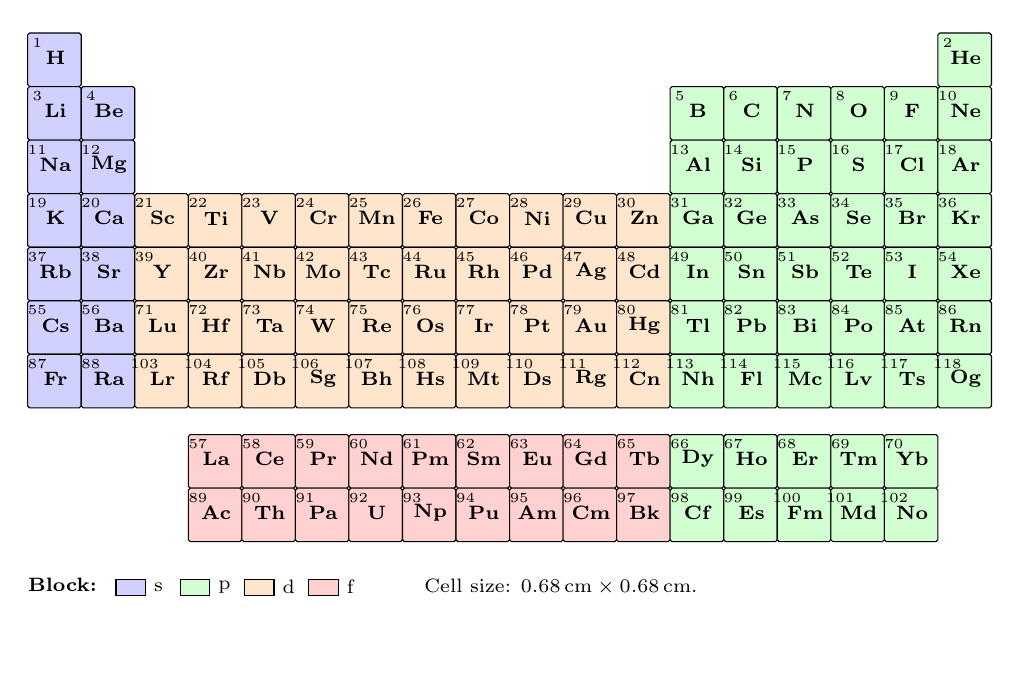
\begin{tikzpicture}[x=0.68cm, y=0.68cm, every node/.style={inner sep=0pt}]
\path[use as bounding box] (0,0.1) rectangle (18,-11.6);
\draw[fill=blue!18, draw=black, rounded corners=0.7pt] (0,0) rectangle (1,-1);
\node at (0.52,-0.46) {\scriptsize \textbf{H}};
\node at (0.18,-0.18) {\tiny 1};
\draw[fill=green!18, draw=black, rounded corners=0.7pt] (17,0) rectangle (18,-1);
\node at (17.52,-0.46) {\scriptsize \textbf{He}};
\node at (17.18,-0.18) {\tiny 2};
\draw[fill=blue!18, draw=black, rounded corners=0.7pt] (0,-1) rectangle (1,-2);
\node at (0.52,-1.46) {\scriptsize \textbf{Li}};
\node at (0.18,-1.18) {\tiny 3};
\draw[fill=blue!18, draw=black, rounded corners=0.7pt] (1,-1) rectangle (2,-2);
\node at (1.52,-1.46) {\scriptsize \textbf{Be}};
\node at (1.18,-1.18) {\tiny 4};
\draw[fill=green!18, draw=black, rounded corners=0.7pt] (12,-1) rectangle (13,-2);
\node at (12.52,-1.46) {\scriptsize \textbf{B}};
\node at (12.18,-1.18) {\tiny 5};
\draw[fill=green!18, draw=black, rounded corners=0.7pt] (13,-1) rectangle (14,-2);
\node at (13.52,-1.46) {\scriptsize \textbf{C}};
\node at (13.18,-1.18) {\tiny 6};
\draw[fill=green!18, draw=black, rounded corners=0.7pt] (14,-1) rectangle (15,-2);
\node at (14.52,-1.46) {\scriptsize \textbf{N}};
\node at (14.18,-1.18) {\tiny 7};
\draw[fill=green!18, draw=black, rounded corners=0.7pt] (15,-1) rectangle (16,-2);
\node at (15.52,-1.46) {\scriptsize \textbf{O}};
\node at (15.18,-1.18) {\tiny 8};
\draw[fill=green!18, draw=black, rounded corners=0.7pt] (16,-1) rectangle (17,-2);
\node at (16.52,-1.46) {\scriptsize \textbf{F}};
\node at (16.18,-1.18) {\tiny 9};
\draw[fill=green!18, draw=black, rounded corners=0.7pt] (17,-1) rectangle (18,-2);
\node at (17.52,-1.46) {\scriptsize \textbf{Ne}};
\node at (17.18,-1.18) {\tiny 10};
\draw[fill=blue!18, draw=black, rounded corners=0.7pt] (0,-2) rectangle (1,-3);
\node at (0.52,-2.46) {\scriptsize \textbf{Na}};
\node at (0.18,-2.18) {\tiny 11};
\draw[fill=blue!18, draw=black, rounded corners=0.7pt] (1,-2) rectangle (2,-3);
\node at (1.52,-2.46) {\scriptsize \textbf{Mg}};
\node at (1.18,-2.18) {\tiny 12};
\draw[fill=green!18, draw=black, rounded corners=0.7pt] (12,-2) rectangle (13,-3);
\node at (12.52,-2.46) {\scriptsize \textbf{Al}};
\node at (12.18,-2.18) {\tiny 13};
\draw[fill=green!18, draw=black, rounded corners=0.7pt] (13,-2) rectangle (14,-3);
\node at (13.52,-2.46) {\scriptsize \textbf{Si}};
\node at (13.18,-2.18) {\tiny 14};
\draw[fill=green!18, draw=black, rounded corners=0.7pt] (14,-2) rectangle (15,-3);
\node at (14.52,-2.46) {\scriptsize \textbf{P}};
\node at (14.18,-2.18) {\tiny 15};
\draw[fill=green!18, draw=black, rounded corners=0.7pt] (15,-2) rectangle (16,-3);
\node at (15.52,-2.46) {\scriptsize \textbf{S}};
\node at (15.18,-2.18) {\tiny 16};
\draw[fill=green!18, draw=black, rounded corners=0.7pt] (16,-2) rectangle (17,-3);
\node at (16.52,-2.46) {\scriptsize \textbf{Cl}};
\node at (16.18,-2.18) {\tiny 17};
\draw[fill=green!18, draw=black, rounded corners=0.7pt] (17,-2) rectangle (18,-3);
\node at (17.52,-2.46) {\scriptsize \textbf{Ar}};
\node at (17.18,-2.18) {\tiny 18};
\draw[fill=blue!18, draw=black, rounded corners=0.7pt] (0,-3) rectangle (1,-4);
\node at (0.52,-3.46) {\scriptsize \textbf{K}};
\node at (0.18,-3.18) {\tiny 19};
\draw[fill=blue!18, draw=black, rounded corners=0.7pt] (1,-3) rectangle (2,-4);
\node at (1.52,-3.46) {\scriptsize \textbf{Ca}};
\node at (1.18,-3.18) {\tiny 20};
\draw[fill=orange!20, draw=black, rounded corners=0.7pt] (2,-3) rectangle (3,-4);
\node at (2.52,-3.46) {\scriptsize \textbf{Sc}};
\node at (2.18,-3.18) {\tiny 21};
\draw[fill=orange!20, draw=black, rounded corners=0.7pt] (3,-3) rectangle (4,-4);
\node at (3.52,-3.46) {\scriptsize \textbf{Ti}};
\node at (3.18,-3.18) {\tiny 22};
\draw[fill=orange!20, draw=black, rounded corners=0.7pt] (4,-3) rectangle (5,-4);
\node at (4.52,-3.46) {\scriptsize \textbf{V}};
\node at (4.18,-3.18) {\tiny 23};
\draw[fill=orange!20, draw=black, rounded corners=0.7pt] (5,-3) rectangle (6,-4);
\node at (5.52,-3.46) {\scriptsize \textbf{Cr}};
\node at (5.18,-3.18) {\tiny 24};
\draw[fill=orange!20, draw=black, rounded corners=0.7pt] (6,-3) rectangle (7,-4);
\node at (6.52,-3.46) {\scriptsize \textbf{Mn}};
\node at (6.18,-3.18) {\tiny 25};
\draw[fill=orange!20, draw=black, rounded corners=0.7pt] (7,-3) rectangle (8,-4);
\node at (7.52,-3.46) {\scriptsize \textbf{Fe}};
\node at (7.18,-3.18) {\tiny 26};
\draw[fill=orange!20, draw=black, rounded corners=0.7pt] (8,-3) rectangle (9,-4);
\node at (8.52,-3.46) {\scriptsize \textbf{Co}};
\node at (8.18,-3.18) {\tiny 27};
\draw[fill=orange!20, draw=black, rounded corners=0.7pt] (9,-3) rectangle (10,-4);
\node at (9.52,-3.46) {\scriptsize \textbf{Ni}};
\node at (9.18,-3.18) {\tiny 28};
\draw[fill=orange!20, draw=black, rounded corners=0.7pt] (10,-3) rectangle (11,-4);
\node at (10.52,-3.46) {\scriptsize \textbf{Cu}};
\node at (10.18,-3.18) {\tiny 29};
\draw[fill=orange!20, draw=black, rounded corners=0.7pt] (11,-3) rectangle (12,-4);
\node at (11.52,-3.46) {\scriptsize \textbf{Zn}};
\node at (11.18,-3.18) {\tiny 30};
\draw[fill=green!18, draw=black, rounded corners=0.7pt] (12,-3) rectangle (13,-4);
\node at (12.52,-3.46) {\scriptsize \textbf{Ga}};
\node at (12.18,-3.18) {\tiny 31};
\draw[fill=green!18, draw=black, rounded corners=0.7pt] (13,-3) rectangle (14,-4);
\node at (13.52,-3.46) {\scriptsize \textbf{Ge}};
\node at (13.18,-3.18) {\tiny 32};
\draw[fill=green!18, draw=black, rounded corners=0.7pt] (14,-3) rectangle (15,-4);
\node at (14.52,-3.46) {\scriptsize \textbf{As}};
\node at (14.18,-3.18) {\tiny 33};
\draw[fill=green!18, draw=black, rounded corners=0.7pt] (15,-3) rectangle (16,-4);
\node at (15.52,-3.46) {\scriptsize \textbf{Se}};
\node at (15.18,-3.18) {\tiny 34};
\draw[fill=green!18, draw=black, rounded corners=0.7pt] (16,-3) rectangle (17,-4);
\node at (16.52,-3.46) {\scriptsize \textbf{Br}};
\node at (16.18,-3.18) {\tiny 35};
\draw[fill=green!18, draw=black, rounded corners=0.7pt] (17,-3) rectangle (18,-4);
\node at (17.52,-3.46) {\scriptsize \textbf{Kr}};
\node at (17.18,-3.18) {\tiny 36};
\draw[fill=blue!18, draw=black, rounded corners=0.7pt] (0,-4) rectangle (1,-5);
\node at (0.52,-4.46) {\scriptsize \textbf{Rb}};
\node at (0.18,-4.18) {\tiny 37};
\draw[fill=blue!18, draw=black, rounded corners=0.7pt] (1,-4) rectangle (2,-5);
\node at (1.52,-4.46) {\scriptsize \textbf{Sr}};
\node at (1.18,-4.18) {\tiny 38};
\draw[fill=orange!20, draw=black, rounded corners=0.7pt] (2,-4) rectangle (3,-5);
\node at (2.52,-4.46) {\scriptsize \textbf{Y}};
\node at (2.18,-4.18) {\tiny 39};
\draw[fill=orange!20, draw=black, rounded corners=0.7pt] (3,-4) rectangle (4,-5);
\node at (3.52,-4.46) {\scriptsize \textbf{Zr}};
\node at (3.18,-4.18) {\tiny 40};
\draw[fill=orange!20, draw=black, rounded corners=0.7pt] (4,-4) rectangle (5,-5);
\node at (4.52,-4.46) {\scriptsize \textbf{Nb}};
\node at (4.18,-4.18) {\tiny 41};
\draw[fill=orange!20, draw=black, rounded corners=0.7pt] (5,-4) rectangle (6,-5);
\node at (5.52,-4.46) {\scriptsize \textbf{Mo}};
\node at (5.18,-4.18) {\tiny 42};
\draw[fill=orange!20, draw=black, rounded corners=0.7pt] (6,-4) rectangle (7,-5);
\node at (6.52,-4.46) {\scriptsize \textbf{Tc}};
\node at (6.18,-4.18) {\tiny 43};
\draw[fill=orange!20, draw=black, rounded corners=0.7pt] (7,-4) rectangle (8,-5);
\node at (7.52,-4.46) {\scriptsize \textbf{Ru}};
\node at (7.18,-4.18) {\tiny 44};
\draw[fill=orange!20, draw=black, rounded corners=0.7pt] (8,-4) rectangle (9,-5);
\node at (8.52,-4.46) {\scriptsize \textbf{Rh}};
\node at (8.18,-4.18) {\tiny 45};
\draw[fill=orange!20, draw=black, rounded corners=0.7pt] (9,-4) rectangle (10,-5);
\node at (9.52,-4.46) {\scriptsize \textbf{Pd}};
\node at (9.18,-4.18) {\tiny 46};
\draw[fill=orange!20, draw=black, rounded corners=0.7pt] (10,-4) rectangle (11,-5);
\node at (10.52,-4.46) {\scriptsize \textbf{Ag}};
\node at (10.18,-4.18) {\tiny 47};
\draw[fill=orange!20, draw=black, rounded corners=0.7pt] (11,-4) rectangle (12,-5);
\node at (11.52,-4.46) {\scriptsize \textbf{Cd}};
\node at (11.18,-4.18) {\tiny 48};
\draw[fill=green!18, draw=black, rounded corners=0.7pt] (12,-4) rectangle (13,-5);
\node at (12.52,-4.46) {\scriptsize \textbf{In}};
\node at (12.18,-4.18) {\tiny 49};
\draw[fill=green!18, draw=black, rounded corners=0.7pt] (13,-4) rectangle (14,-5);
\node at (13.52,-4.46) {\scriptsize \textbf{Sn}};
\node at (13.18,-4.18) {\tiny 50};
\draw[fill=green!18, draw=black, rounded corners=0.7pt] (14,-4) rectangle (15,-5);
\node at (14.52,-4.46) {\scriptsize \textbf{Sb}};
\node at (14.18,-4.18) {\tiny 51};
\draw[fill=green!18, draw=black, rounded corners=0.7pt] (15,-4) rectangle (16,-5);
\node at (15.52,-4.46) {\scriptsize \textbf{Te}};
\node at (15.18,-4.18) {\tiny 52};
\draw[fill=green!18, draw=black, rounded corners=0.7pt] (16,-4) rectangle (17,-5);
\node at (16.52,-4.46) {\scriptsize \textbf{I}};
\node at (16.18,-4.18) {\tiny 53};
\draw[fill=green!18, draw=black, rounded corners=0.7pt] (17,-4) rectangle (18,-5);
\node at (17.52,-4.46) {\scriptsize \textbf{Xe}};
\node at (17.18,-4.18) {\tiny 54};
\draw[fill=blue!18, draw=black, rounded corners=0.7pt] (0,-5) rectangle (1,-6);
\node at (0.52,-5.46) {\scriptsize \textbf{Cs}};
\node at (0.18,-5.18) {\tiny 55};
\draw[fill=blue!18, draw=black, rounded corners=0.7pt] (1,-5) rectangle (2,-6);
\node at (1.52,-5.46) {\scriptsize \textbf{Ba}};
\node at (1.18,-5.18) {\tiny 56};
\draw[fill=orange!20, draw=black, rounded corners=0.7pt] (2,-5) rectangle (3,-6);
\node at (2.52,-5.46) {\scriptsize \textbf{Lu}};
\node at (2.18,-5.18) {\tiny 71};
\draw[fill=orange!20, draw=black, rounded corners=0.7pt] (3,-5) rectangle (4,-6);
\node at (3.52,-5.46) {\scriptsize \textbf{Hf}};
\node at (3.18,-5.18) {\tiny 72};
\draw[fill=orange!20, draw=black, rounded corners=0.7pt] (4,-5) rectangle (5,-6);
\node at (4.52,-5.46) {\scriptsize \textbf{Ta}};
\node at (4.18,-5.18) {\tiny 73};
\draw[fill=orange!20, draw=black, rounded corners=0.7pt] (5,-5) rectangle (6,-6);
\node at (5.52,-5.46) {\scriptsize \textbf{W}};
\node at (5.18,-5.18) {\tiny 74};
\draw[fill=orange!20, draw=black, rounded corners=0.7pt] (6,-5) rectangle (7,-6);
\node at (6.52,-5.46) {\scriptsize \textbf{Re}};
\node at (6.18,-5.18) {\tiny 75};
\draw[fill=orange!20, draw=black, rounded corners=0.7pt] (7,-5) rectangle (8,-6);
\node at (7.52,-5.46) {\scriptsize \textbf{Os}};
\node at (7.18,-5.18) {\tiny 76};
\draw[fill=orange!20, draw=black, rounded corners=0.7pt] (8,-5) rectangle (9,-6);
\node at (8.52,-5.46) {\scriptsize \textbf{Ir}};
\node at (8.18,-5.18) {\tiny 77};
\draw[fill=orange!20, draw=black, rounded corners=0.7pt] (9,-5) rectangle (10,-6);
\node at (9.52,-5.46) {\scriptsize \textbf{Pt}};
\node at (9.18,-5.18) {\tiny 78};
\draw[fill=orange!20, draw=black, rounded corners=0.7pt] (10,-5) rectangle (11,-6);
\node at (10.52,-5.46) {\scriptsize \textbf{Au}};
\node at (10.18,-5.18) {\tiny 79};
\draw[fill=orange!20, draw=black, rounded corners=0.7pt] (11,-5) rectangle (12,-6);
\node at (11.52,-5.46) {\scriptsize \textbf{Hg}};
\node at (11.18,-5.18) {\tiny 80};
\draw[fill=green!18, draw=black, rounded corners=0.7pt] (12,-5) rectangle (13,-6);
\node at (12.52,-5.46) {\scriptsize \textbf{Tl}};
\node at (12.18,-5.18) {\tiny 81};
\draw[fill=green!18, draw=black, rounded corners=0.7pt] (13,-5) rectangle (14,-6);
\node at (13.52,-5.46) {\scriptsize \textbf{Pb}};
\node at (13.18,-5.18) {\tiny 82};
\draw[fill=green!18, draw=black, rounded corners=0.7pt] (14,-5) rectangle (15,-6);
\node at (14.52,-5.46) {\scriptsize \textbf{Bi}};
\node at (14.18,-5.18) {\tiny 83};
\draw[fill=green!18, draw=black, rounded corners=0.7pt] (15,-5) rectangle (16,-6);
\node at (15.52,-5.46) {\scriptsize \textbf{Po}};
\node at (15.18,-5.18) {\tiny 84};
\draw[fill=green!18, draw=black, rounded corners=0.7pt] (16,-5) rectangle (17,-6);
\node at (16.52,-5.46) {\scriptsize \textbf{At}};
\node at (16.18,-5.18) {\tiny 85};
\draw[fill=green!18, draw=black, rounded corners=0.7pt] (17,-5) rectangle (18,-6);
\node at (17.52,-5.46) {\scriptsize \textbf{Rn}};
\node at (17.18,-5.18) {\tiny 86};
\draw[fill=blue!18, draw=black, rounded corners=0.7pt] (0,-6) rectangle (1,-7);
\node at (0.52,-6.46) {\scriptsize \textbf{Fr}};
\node at (0.18,-6.18) {\tiny 87};
\draw[fill=blue!18, draw=black, rounded corners=0.7pt] (1,-6) rectangle (2,-7);
\node at (1.52,-6.46) {\scriptsize \textbf{Ra}};
\node at (1.18,-6.18) {\tiny 88};
\draw[fill=orange!20, draw=black, rounded corners=0.7pt] (2,-6) rectangle (3,-7);
\node at (2.52,-6.46) {\scriptsize \textbf{Lr}};
\node at (2.18,-6.18) {\tiny 103};
\draw[fill=orange!20, draw=black, rounded corners=0.7pt] (3,-6) rectangle (4,-7);
\node at (3.52,-6.46) {\scriptsize \textbf{Rf}};
\node at (3.18,-6.18) {\tiny 104};
\draw[fill=orange!20, draw=black, rounded corners=0.7pt] (4,-6) rectangle (5,-7);
\node at (4.52,-6.46) {\scriptsize \textbf{Db}};
\node at (4.18,-6.18) {\tiny 105};
\draw[fill=orange!20, draw=black, rounded corners=0.7pt] (5,-6) rectangle (6,-7);
\node at (5.52,-6.46) {\scriptsize \textbf{Sg}};
\node at (5.18,-6.18) {\tiny 106};
\draw[fill=orange!20, draw=black, rounded corners=0.7pt] (6,-6) rectangle (7,-7);
\node at (6.52,-6.46) {\scriptsize \textbf{Bh}};
\node at (6.18,-6.18) {\tiny 107};
\draw[fill=orange!20, draw=black, rounded corners=0.7pt] (7,-6) rectangle (8,-7);
\node at (7.52,-6.46) {\scriptsize \textbf{Hs}};
\node at (7.18,-6.18) {\tiny 108};
\draw[fill=orange!20, draw=black, rounded corners=0.7pt] (8,-6) rectangle (9,-7);
\node at (8.52,-6.46) {\scriptsize \textbf{Mt}};
\node at (8.18,-6.18) {\tiny 109};
\draw[fill=orange!20, draw=black, rounded corners=0.7pt] (9,-6) rectangle (10,-7);
\node at (9.52,-6.46) {\scriptsize \textbf{Ds}};
\node at (9.18,-6.18) {\tiny 110};
\draw[fill=orange!20, draw=black, rounded corners=0.7pt] (10,-6) rectangle (11,-7);
\node at (10.52,-6.46) {\scriptsize \textbf{Rg}};
\node at (10.18,-6.18) {\tiny 111};
\draw[fill=orange!20, draw=black, rounded corners=0.7pt] (11,-6) rectangle (12,-7);
\node at (11.52,-6.46) {\scriptsize \textbf{Cn}};
\node at (11.18,-6.18) {\tiny 112};
\draw[fill=green!18, draw=black, rounded corners=0.7pt] (12,-6) rectangle (13,-7);
\node at (12.52,-6.46) {\scriptsize \textbf{Nh}};
\node at (12.18,-6.18) {\tiny 113};
\draw[fill=green!18, draw=black, rounded corners=0.7pt] (13,-6) rectangle (14,-7);
\node at (13.52,-6.46) {\scriptsize \textbf{Fl}};
\node at (13.18,-6.18) {\tiny 114};
\draw[fill=green!18, draw=black, rounded corners=0.7pt] (14,-6) rectangle (15,-7);
\node at (14.52,-6.46) {\scriptsize \textbf{Mc}};
\node at (14.18,-6.18) {\tiny 115};
\draw[fill=green!18, draw=black, rounded corners=0.7pt] (15,-6) rectangle (16,-7);
\node at (15.52,-6.46) {\scriptsize \textbf{Lv}};
\node at (15.18,-6.18) {\tiny 116};
\draw[fill=green!18, draw=black, rounded corners=0.7pt] (16,-6) rectangle (17,-7);
\node at (16.52,-6.46) {\scriptsize \textbf{Ts}};
\node at (16.18,-6.18) {\tiny 117};
\draw[fill=green!18, draw=black, rounded corners=0.7pt] (17,-6) rectangle (18,-7);
\node at (17.52,-6.46) {\scriptsize \textbf{Og}};
\node at (17.18,-6.18) {\tiny 118};
\draw[fill=red!18, draw=black, rounded corners=0.7pt] (3,-7.5) rectangle (4,-8.5);
\node at (3.52,-7.96) {\scriptsize \textbf{La}};
\node at (3.18,-7.68) {\tiny 57};
\draw[fill=red!18, draw=black, rounded corners=0.7pt] (4,-7.5) rectangle (5,-8.5);
\node at (4.52,-7.96) {\scriptsize \textbf{Ce}};
\node at (4.18,-7.68) {\tiny 58};
\draw[fill=red!18, draw=black, rounded corners=0.7pt] (5,-7.5) rectangle (6,-8.5);
\node at (5.52,-7.96) {\scriptsize \textbf{Pr}};
\node at (5.18,-7.68) {\tiny 59};
\draw[fill=red!18, draw=black, rounded corners=0.7pt] (6,-7.5) rectangle (7,-8.5);
\node at (6.52,-7.96) {\scriptsize \textbf{Nd}};
\node at (6.18,-7.68) {\tiny 60};
\draw[fill=red!18, draw=black, rounded corners=0.7pt] (7,-7.5) rectangle (8,-8.5);
\node at (7.52,-7.96) {\scriptsize \textbf{Pm}};
\node at (7.18,-7.68) {\tiny 61};
\draw[fill=red!18, draw=black, rounded corners=0.7pt] (8,-7.5) rectangle (9,-8.5);
\node at (8.52,-7.96) {\scriptsize \textbf{Sm}};
\node at (8.18,-7.68) {\tiny 62};
\draw[fill=red!18, draw=black, rounded corners=0.7pt] (9,-7.5) rectangle (10,-8.5);
\node at (9.52,-7.96) {\scriptsize \textbf{Eu}};
\node at (9.18,-7.68) {\tiny 63};
\draw[fill=red!18, draw=black, rounded corners=0.7pt] (10,-7.5) rectangle (11,-8.5);
\node at (10.52,-7.96) {\scriptsize \textbf{Gd}};
\node at (10.18,-7.68) {\tiny 64};
\draw[fill=red!18, draw=black, rounded corners=0.7pt] (11,-7.5) rectangle (12,-8.5);
\node at (11.52,-7.96) {\scriptsize \textbf{Tb}};
\node at (11.18,-7.68) {\tiny 65};
\draw[fill=green!18, draw=black, rounded corners=0.7pt] (12,-7.5) rectangle (13,-8.5);
\node at (12.52,-7.96) {\scriptsize \textbf{Dy}};
\node at (12.18,-7.68) {\tiny 66};
\draw[fill=green!18, draw=black, rounded corners=0.7pt] (13,-7.5) rectangle (14,-8.5);
\node at (13.52,-7.96) {\scriptsize \textbf{Ho}};
\node at (13.18,-7.68) {\tiny 67};
\draw[fill=green!18, draw=black, rounded corners=0.7pt] (14,-7.5) rectangle (15,-8.5);
\node at (14.52,-7.96) {\scriptsize \textbf{Er}};
\node at (14.18,-7.68) {\tiny 68};
\draw[fill=green!18, draw=black, rounded corners=0.7pt] (15,-7.5) rectangle (16,-8.5);
\node at (15.52,-7.96) {\scriptsize \textbf{Tm}};
\node at (15.18,-7.68) {\tiny 69};
\draw[fill=green!18, draw=black, rounded corners=0.7pt] (16,-7.5) rectangle (17,-8.5);
\node at (16.52,-7.96) {\scriptsize \textbf{Yb}};
\node at (16.18,-7.68) {\tiny 70};
\draw[fill=red!18, draw=black, rounded corners=0.7pt] (3,-8.5) rectangle (4,-9.5);
\node at (3.52,-8.96) {\scriptsize \textbf{Ac}};
\node at (3.18,-8.68) {\tiny 89};
\draw[fill=red!18, draw=black, rounded corners=0.7pt] (4,-8.5) rectangle (5,-9.5);
\node at (4.52,-8.96) {\scriptsize \textbf{Th}};
\node at (4.18,-8.68) {\tiny 90};
\draw[fill=red!18, draw=black, rounded corners=0.7pt] (5,-8.5) rectangle (6,-9.5);
\node at (5.52,-8.96) {\scriptsize \textbf{Pa}};
\node at (5.18,-8.68) {\tiny 91};
\draw[fill=red!18, draw=black, rounded corners=0.7pt] (6,-8.5) rectangle (7,-9.5);
\node at (6.52,-8.96) {\scriptsize \textbf{U}};
\node at (6.18,-8.68) {\tiny 92};
\draw[fill=red!18, draw=black, rounded corners=0.7pt] (7,-8.5) rectangle (8,-9.5);
\node at (7.52,-8.96) {\scriptsize \textbf{Np}};
\node at (7.18,-8.68) {\tiny 93};
\draw[fill=red!18, draw=black, rounded corners=0.7pt] (8,-8.5) rectangle (9,-9.5);
\node at (8.52,-8.96) {\scriptsize \textbf{Pu}};
\node at (8.18,-8.68) {\tiny 94};
\draw[fill=red!18, draw=black, rounded corners=0.7pt] (9,-8.5) rectangle (10,-9.5);
\node at (9.52,-8.96) {\scriptsize \textbf{Am}};
\node at (9.18,-8.68) {\tiny 95};
\draw[fill=red!18, draw=black, rounded corners=0.7pt] (10,-8.5) rectangle (11,-9.5);
\node at (10.52,-8.96) {\scriptsize \textbf{Cm}};
\node at (10.18,-8.68) {\tiny 96};
\draw[fill=red!18, draw=black, rounded corners=0.7pt] (11,-8.5) rectangle (12,-9.5);
\node at (11.52,-8.96) {\scriptsize \textbf{Bk}};
\node at (11.18,-8.68) {\tiny 97};
\draw[fill=green!18, draw=black, rounded corners=0.7pt] (12,-8.5) rectangle (13,-9.5);
\node at (12.52,-8.96) {\scriptsize \textbf{Cf}};
\node at (12.18,-8.68) {\tiny 98};
\draw[fill=green!18, draw=black, rounded corners=0.7pt] (13,-8.5) rectangle (14,-9.5);
\node at (13.52,-8.96) {\scriptsize \textbf{Es}};
\node at (13.18,-8.68) {\tiny 99};
\draw[fill=green!18, draw=black, rounded corners=0.7pt] (14,-8.5) rectangle (15,-9.5);
\node at (14.52,-8.96) {\scriptsize \textbf{Fm}};
\node at (14.18,-8.68) {\tiny 100};
\draw[fill=green!18, draw=black, rounded corners=0.7pt] (15,-8.5) rectangle (16,-9.5);
\node at (15.52,-8.96) {\scriptsize \textbf{Md}};
\node at (15.18,-8.68) {\tiny 101};
\draw[fill=green!18, draw=black, rounded corners=0.7pt] (16,-8.5) rectangle (17,-9.5);
\node at (16.52,-8.96) {\scriptsize \textbf{No}};
\node at (16.18,-8.68) {\tiny 102};
\node[anchor=west] at (0.0,-10.309999999999999) {\scriptsize \textbf{Block:}};
\draw[fill=blue!18, draw=black] (1.65,-10.2) rectangle (2.2,-10.5);
\node[anchor=west] at (2.3499999999999996,-10.35) {\scriptsize s};
\draw[fill=green!18, draw=black] (2.8499999999999996,-10.2) rectangle (3.3999999999999995,-10.5);
\node[anchor=west] at (3.55,-10.35) {\scriptsize p};
\draw[fill=orange!20, draw=black] (4.05,-10.2) rectangle (4.6,-10.5);
\node[anchor=west] at (4.75,-10.35) {\scriptsize d};
\draw[fill=red!18, draw=black] (5.25,-10.2) rectangle (5.8,-10.5);
\node[anchor=west] at (5.95,-10.35) {\scriptsize f};
\node[anchor=west] at (7.4,-10.35) {\scriptsize Cell size: $0.68\,\mathrm{cm}\times0.68\,\mathrm{cm}$.};
\end{tikzpicture}
\caption{Variant 0: classical periodic table used as the reference. Element positions, symbols, and positive-$Z$ indexing follow the IUPAC source basis cited in the manuscript; colors encode only the matter orbital-block structure.}
\label{fig:ptable-standard}
\end{figure}


This figure is a baseline. It shows established orbital-block structure and no antimatter evidence.

\subsection{Split-Cell Antimatter Periodic Table}

\begin{figure}[H]
\centering
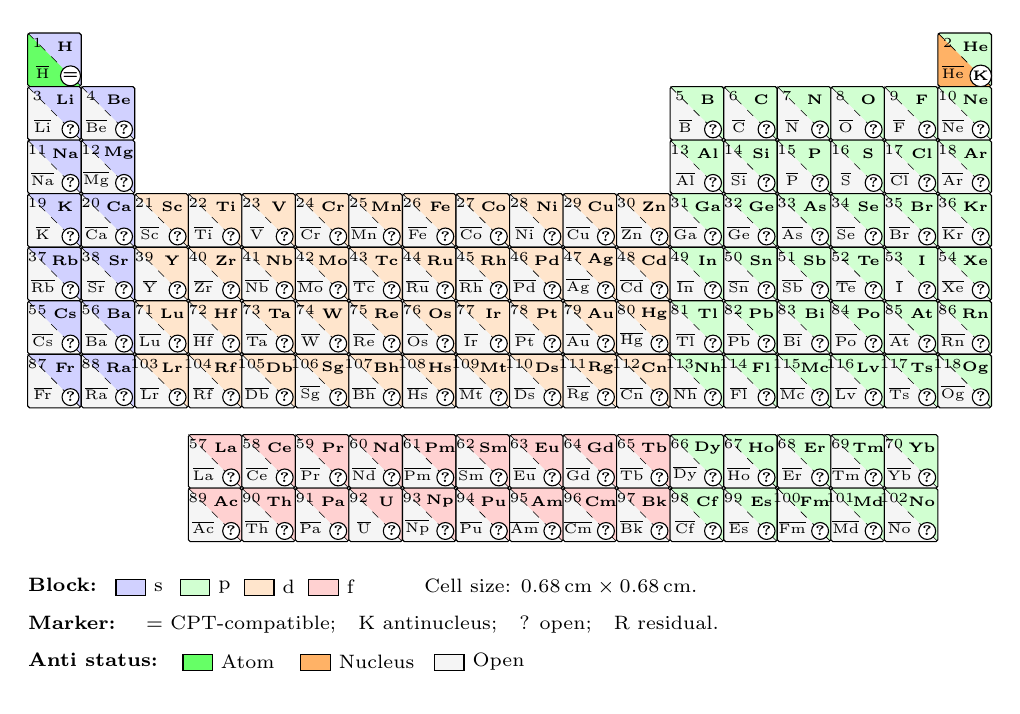
\begin{tikzpicture}[x=0.68cm, y=0.68cm, every node/.style={inner sep=0pt}]
\path[use as bounding box] (0,0.1) rectangle (18,-12.2);
\fill[blue!18, rounded corners=0.7pt] (0,0) -- (1,0) -- (1,-1) -- cycle;
\fill[green!60, rounded corners=0.7pt] (0,0) -- (0,-1) -- (1,-1) -- cycle;
\draw[black, rounded corners=0.7pt] (0,0) rectangle (1,-1);
\draw[black, dashed, very thin] (0,0) -- (1,-1);
\node at (0.7,-0.25) {\tiny \textbf{H}};
\node at (0.28,-0.73) {\tiny \textbf{$\overline{\mathrm{H}}$}};
\node at (0.18,-0.18) {\tiny 1};
\node[fill=white, draw=black, circle, inner sep=0.4pt] at (0.8,-0.8) {\tiny \textbf{=}};
\fill[green!18, rounded corners=0.7pt] (17,0) -- (18,0) -- (18,-1) -- cycle;
\fill[orange!60, rounded corners=0.7pt] (17,0) -- (17,-1) -- (18,-1) -- cycle;
\draw[black, rounded corners=0.7pt] (17,0) rectangle (18,-1);
\draw[black, dashed, very thin] (17,0) -- (18,-1);
\node at (17.7,-0.25) {\tiny \textbf{He}};
\node at (17.28,-0.73) {\tiny \textbf{$\overline{\mathrm{He}}$}};
\node at (17.18,-0.18) {\tiny 2};
\node[fill=white, draw=black, circle, inner sep=0.4pt] at (17.8,-0.8) {\tiny \textbf{K}};
\fill[blue!18, rounded corners=0.7pt] (0,-1) -- (1,-1) -- (1,-2) -- cycle;
\fill[gray!8, rounded corners=0.7pt] (0,-1) -- (0,-2) -- (1,-2) -- cycle;
\draw[black, rounded corners=0.7pt] (0,-1) rectangle (1,-2);
\draw[black, dashed, very thin] (0,-1) -- (1,-2);
\node at (0.7,-1.25) {\tiny \textbf{Li}};
\node at (0.28,-1.73) {\tiny \textbf{$\overline{\mathrm{Li}}$}};
\node at (0.18,-1.18) {\tiny 3};
\node[fill=white, draw=black, circle, inner sep=0.4pt] at (0.8,-1.8) {\tiny \textbf{?}};
\fill[blue!18, rounded corners=0.7pt] (1,-1) -- (2,-1) -- (2,-2) -- cycle;
\fill[gray!8, rounded corners=0.7pt] (1,-1) -- (1,-2) -- (2,-2) -- cycle;
\draw[black, rounded corners=0.7pt] (1,-1) rectangle (2,-2);
\draw[black, dashed, very thin] (1,-1) -- (2,-2);
\node at (1.7,-1.25) {\tiny \textbf{Be}};
\node at (1.28,-1.73) {\tiny \textbf{$\overline{\mathrm{Be}}$}};
\node at (1.18,-1.18) {\tiny 4};
\node[fill=white, draw=black, circle, inner sep=0.4pt] at (1.8,-1.8) {\tiny \textbf{?}};
\fill[green!18, rounded corners=0.7pt] (12,-1) -- (13,-1) -- (13,-2) -- cycle;
\fill[gray!8, rounded corners=0.7pt] (12,-1) -- (12,-2) -- (13,-2) -- cycle;
\draw[black, rounded corners=0.7pt] (12,-1) rectangle (13,-2);
\draw[black, dashed, very thin] (12,-1) -- (13,-2);
\node at (12.7,-1.25) {\tiny \textbf{B}};
\node at (12.28,-1.73) {\tiny \textbf{$\overline{\mathrm{B}}$}};
\node at (12.18,-1.18) {\tiny 5};
\node[fill=white, draw=black, circle, inner sep=0.4pt] at (12.8,-1.8) {\tiny \textbf{?}};
\fill[green!18, rounded corners=0.7pt] (13,-1) -- (14,-1) -- (14,-2) -- cycle;
\fill[gray!8, rounded corners=0.7pt] (13,-1) -- (13,-2) -- (14,-2) -- cycle;
\draw[black, rounded corners=0.7pt] (13,-1) rectangle (14,-2);
\draw[black, dashed, very thin] (13,-1) -- (14,-2);
\node at (13.7,-1.25) {\tiny \textbf{C}};
\node at (13.28,-1.73) {\tiny \textbf{$\overline{\mathrm{C}}$}};
\node at (13.18,-1.18) {\tiny 6};
\node[fill=white, draw=black, circle, inner sep=0.4pt] at (13.8,-1.8) {\tiny \textbf{?}};
\fill[green!18, rounded corners=0.7pt] (14,-1) -- (15,-1) -- (15,-2) -- cycle;
\fill[gray!8, rounded corners=0.7pt] (14,-1) -- (14,-2) -- (15,-2) -- cycle;
\draw[black, rounded corners=0.7pt] (14,-1) rectangle (15,-2);
\draw[black, dashed, very thin] (14,-1) -- (15,-2);
\node at (14.7,-1.25) {\tiny \textbf{N}};
\node at (14.28,-1.73) {\tiny \textbf{$\overline{\mathrm{N}}$}};
\node at (14.18,-1.18) {\tiny 7};
\node[fill=white, draw=black, circle, inner sep=0.4pt] at (14.8,-1.8) {\tiny \textbf{?}};
\fill[green!18, rounded corners=0.7pt] (15,-1) -- (16,-1) -- (16,-2) -- cycle;
\fill[gray!8, rounded corners=0.7pt] (15,-1) -- (15,-2) -- (16,-2) -- cycle;
\draw[black, rounded corners=0.7pt] (15,-1) rectangle (16,-2);
\draw[black, dashed, very thin] (15,-1) -- (16,-2);
\node at (15.7,-1.25) {\tiny \textbf{O}};
\node at (15.28,-1.73) {\tiny \textbf{$\overline{\mathrm{O}}$}};
\node at (15.18,-1.18) {\tiny 8};
\node[fill=white, draw=black, circle, inner sep=0.4pt] at (15.8,-1.8) {\tiny \textbf{?}};
\fill[green!18, rounded corners=0.7pt] (16,-1) -- (17,-1) -- (17,-2) -- cycle;
\fill[gray!8, rounded corners=0.7pt] (16,-1) -- (16,-2) -- (17,-2) -- cycle;
\draw[black, rounded corners=0.7pt] (16,-1) rectangle (17,-2);
\draw[black, dashed, very thin] (16,-1) -- (17,-2);
\node at (16.7,-1.25) {\tiny \textbf{F}};
\node at (16.28,-1.73) {\tiny \textbf{$\overline{\mathrm{F}}$}};
\node at (16.18,-1.18) {\tiny 9};
\node[fill=white, draw=black, circle, inner sep=0.4pt] at (16.8,-1.8) {\tiny \textbf{?}};
\fill[green!18, rounded corners=0.7pt] (17,-1) -- (18,-1) -- (18,-2) -- cycle;
\fill[gray!8, rounded corners=0.7pt] (17,-1) -- (17,-2) -- (18,-2) -- cycle;
\draw[black, rounded corners=0.7pt] (17,-1) rectangle (18,-2);
\draw[black, dashed, very thin] (17,-1) -- (18,-2);
\node at (17.7,-1.25) {\tiny \textbf{Ne}};
\node at (17.28,-1.73) {\tiny \textbf{$\overline{\mathrm{Ne}}$}};
\node at (17.18,-1.18) {\tiny 10};
\node[fill=white, draw=black, circle, inner sep=0.4pt] at (17.8,-1.8) {\tiny \textbf{?}};
\fill[blue!18, rounded corners=0.7pt] (0,-2) -- (1,-2) -- (1,-3) -- cycle;
\fill[gray!8, rounded corners=0.7pt] (0,-2) -- (0,-3) -- (1,-3) -- cycle;
\draw[black, rounded corners=0.7pt] (0,-2) rectangle (1,-3);
\draw[black, dashed, very thin] (0,-2) -- (1,-3);
\node at (0.7,-2.25) {\tiny \textbf{Na}};
\node at (0.28,-2.73) {\tiny \textbf{$\overline{\mathrm{Na}}$}};
\node at (0.18,-2.18) {\tiny 11};
\node[fill=white, draw=black, circle, inner sep=0.4pt] at (0.8,-2.8) {\tiny \textbf{?}};
\fill[blue!18, rounded corners=0.7pt] (1,-2) -- (2,-2) -- (2,-3) -- cycle;
\fill[gray!8, rounded corners=0.7pt] (1,-2) -- (1,-3) -- (2,-3) -- cycle;
\draw[black, rounded corners=0.7pt] (1,-2) rectangle (2,-3);
\draw[black, dashed, very thin] (1,-2) -- (2,-3);
\node at (1.7,-2.25) {\tiny \textbf{Mg}};
\node at (1.28,-2.73) {\tiny \textbf{$\overline{\mathrm{Mg}}$}};
\node at (1.18,-2.18) {\tiny 12};
\node[fill=white, draw=black, circle, inner sep=0.4pt] at (1.8,-2.8) {\tiny \textbf{?}};
\fill[green!18, rounded corners=0.7pt] (12,-2) -- (13,-2) -- (13,-3) -- cycle;
\fill[gray!8, rounded corners=0.7pt] (12,-2) -- (12,-3) -- (13,-3) -- cycle;
\draw[black, rounded corners=0.7pt] (12,-2) rectangle (13,-3);
\draw[black, dashed, very thin] (12,-2) -- (13,-3);
\node at (12.7,-2.25) {\tiny \textbf{Al}};
\node at (12.28,-2.73) {\tiny \textbf{$\overline{\mathrm{Al}}$}};
\node at (12.18,-2.18) {\tiny 13};
\node[fill=white, draw=black, circle, inner sep=0.4pt] at (12.8,-2.8) {\tiny \textbf{?}};
\fill[green!18, rounded corners=0.7pt] (13,-2) -- (14,-2) -- (14,-3) -- cycle;
\fill[gray!8, rounded corners=0.7pt] (13,-2) -- (13,-3) -- (14,-3) -- cycle;
\draw[black, rounded corners=0.7pt] (13,-2) rectangle (14,-3);
\draw[black, dashed, very thin] (13,-2) -- (14,-3);
\node at (13.7,-2.25) {\tiny \textbf{Si}};
\node at (13.28,-2.73) {\tiny \textbf{$\overline{\mathrm{Si}}$}};
\node at (13.18,-2.18) {\tiny 14};
\node[fill=white, draw=black, circle, inner sep=0.4pt] at (13.8,-2.8) {\tiny \textbf{?}};
\fill[green!18, rounded corners=0.7pt] (14,-2) -- (15,-2) -- (15,-3) -- cycle;
\fill[gray!8, rounded corners=0.7pt] (14,-2) -- (14,-3) -- (15,-3) -- cycle;
\draw[black, rounded corners=0.7pt] (14,-2) rectangle (15,-3);
\draw[black, dashed, very thin] (14,-2) -- (15,-3);
\node at (14.7,-2.25) {\tiny \textbf{P}};
\node at (14.28,-2.73) {\tiny \textbf{$\overline{\mathrm{P}}$}};
\node at (14.18,-2.18) {\tiny 15};
\node[fill=white, draw=black, circle, inner sep=0.4pt] at (14.8,-2.8) {\tiny \textbf{?}};
\fill[green!18, rounded corners=0.7pt] (15,-2) -- (16,-2) -- (16,-3) -- cycle;
\fill[gray!8, rounded corners=0.7pt] (15,-2) -- (15,-3) -- (16,-3) -- cycle;
\draw[black, rounded corners=0.7pt] (15,-2) rectangle (16,-3);
\draw[black, dashed, very thin] (15,-2) -- (16,-3);
\node at (15.7,-2.25) {\tiny \textbf{S}};
\node at (15.28,-2.73) {\tiny \textbf{$\overline{\mathrm{S}}$}};
\node at (15.18,-2.18) {\tiny 16};
\node[fill=white, draw=black, circle, inner sep=0.4pt] at (15.8,-2.8) {\tiny \textbf{?}};
\fill[green!18, rounded corners=0.7pt] (16,-2) -- (17,-2) -- (17,-3) -- cycle;
\fill[gray!8, rounded corners=0.7pt] (16,-2) -- (16,-3) -- (17,-3) -- cycle;
\draw[black, rounded corners=0.7pt] (16,-2) rectangle (17,-3);
\draw[black, dashed, very thin] (16,-2) -- (17,-3);
\node at (16.7,-2.25) {\tiny \textbf{Cl}};
\node at (16.28,-2.73) {\tiny \textbf{$\overline{\mathrm{Cl}}$}};
\node at (16.18,-2.18) {\tiny 17};
\node[fill=white, draw=black, circle, inner sep=0.4pt] at (16.8,-2.8) {\tiny \textbf{?}};
\fill[green!18, rounded corners=0.7pt] (17,-2) -- (18,-2) -- (18,-3) -- cycle;
\fill[gray!8, rounded corners=0.7pt] (17,-2) -- (17,-3) -- (18,-3) -- cycle;
\draw[black, rounded corners=0.7pt] (17,-2) rectangle (18,-3);
\draw[black, dashed, very thin] (17,-2) -- (18,-3);
\node at (17.7,-2.25) {\tiny \textbf{Ar}};
\node at (17.28,-2.73) {\tiny \textbf{$\overline{\mathrm{Ar}}$}};
\node at (17.18,-2.18) {\tiny 18};
\node[fill=white, draw=black, circle, inner sep=0.4pt] at (17.8,-2.8) {\tiny \textbf{?}};
\fill[blue!18, rounded corners=0.7pt] (0,-3) -- (1,-3) -- (1,-4) -- cycle;
\fill[gray!8, rounded corners=0.7pt] (0,-3) -- (0,-4) -- (1,-4) -- cycle;
\draw[black, rounded corners=0.7pt] (0,-3) rectangle (1,-4);
\draw[black, dashed, very thin] (0,-3) -- (1,-4);
\node at (0.7,-3.25) {\tiny \textbf{K}};
\node at (0.28,-3.73) {\tiny \textbf{$\overline{\mathrm{K}}$}};
\node at (0.18,-3.18) {\tiny 19};
\node[fill=white, draw=black, circle, inner sep=0.4pt] at (0.8,-3.8) {\tiny \textbf{?}};
\fill[blue!18, rounded corners=0.7pt] (1,-3) -- (2,-3) -- (2,-4) -- cycle;
\fill[gray!8, rounded corners=0.7pt] (1,-3) -- (1,-4) -- (2,-4) -- cycle;
\draw[black, rounded corners=0.7pt] (1,-3) rectangle (2,-4);
\draw[black, dashed, very thin] (1,-3) -- (2,-4);
\node at (1.7,-3.25) {\tiny \textbf{Ca}};
\node at (1.28,-3.73) {\tiny \textbf{$\overline{\mathrm{Ca}}$}};
\node at (1.18,-3.18) {\tiny 20};
\node[fill=white, draw=black, circle, inner sep=0.4pt] at (1.8,-3.8) {\tiny \textbf{?}};
\fill[orange!20, rounded corners=0.7pt] (2,-3) -- (3,-3) -- (3,-4) -- cycle;
\fill[gray!8, rounded corners=0.7pt] (2,-3) -- (2,-4) -- (3,-4) -- cycle;
\draw[black, rounded corners=0.7pt] (2,-3) rectangle (3,-4);
\draw[black, dashed, very thin] (2,-3) -- (3,-4);
\node at (2.7,-3.25) {\tiny \textbf{Sc}};
\node at (2.2800000000000002,-3.73) {\tiny \textbf{$\overline{\mathrm{Sc}}$}};
\node at (2.18,-3.18) {\tiny 21};
\node[fill=white, draw=black, circle, inner sep=0.4pt] at (2.8,-3.8) {\tiny \textbf{?}};
\fill[orange!20, rounded corners=0.7pt] (3,-3) -- (4,-3) -- (4,-4) -- cycle;
\fill[gray!8, rounded corners=0.7pt] (3,-3) -- (3,-4) -- (4,-4) -- cycle;
\draw[black, rounded corners=0.7pt] (3,-3) rectangle (4,-4);
\draw[black, dashed, very thin] (3,-3) -- (4,-4);
\node at (3.7,-3.25) {\tiny \textbf{Ti}};
\node at (3.2800000000000002,-3.73) {\tiny \textbf{$\overline{\mathrm{Ti}}$}};
\node at (3.18,-3.18) {\tiny 22};
\node[fill=white, draw=black, circle, inner sep=0.4pt] at (3.8,-3.8) {\tiny \textbf{?}};
\fill[orange!20, rounded corners=0.7pt] (4,-3) -- (5,-3) -- (5,-4) -- cycle;
\fill[gray!8, rounded corners=0.7pt] (4,-3) -- (4,-4) -- (5,-4) -- cycle;
\draw[black, rounded corners=0.7pt] (4,-3) rectangle (5,-4);
\draw[black, dashed, very thin] (4,-3) -- (5,-4);
\node at (4.7,-3.25) {\tiny \textbf{V}};
\node at (4.28,-3.73) {\tiny \textbf{$\overline{\mathrm{V}}$}};
\node at (4.18,-3.18) {\tiny 23};
\node[fill=white, draw=black, circle, inner sep=0.4pt] at (4.8,-3.8) {\tiny \textbf{?}};
\fill[orange!20, rounded corners=0.7pt] (5,-3) -- (6,-3) -- (6,-4) -- cycle;
\fill[gray!8, rounded corners=0.7pt] (5,-3) -- (5,-4) -- (6,-4) -- cycle;
\draw[black, rounded corners=0.7pt] (5,-3) rectangle (6,-4);
\draw[black, dashed, very thin] (5,-3) -- (6,-4);
\node at (5.7,-3.25) {\tiny \textbf{Cr}};
\node at (5.28,-3.73) {\tiny \textbf{$\overline{\mathrm{Cr}}$}};
\node at (5.18,-3.18) {\tiny 24};
\node[fill=white, draw=black, circle, inner sep=0.4pt] at (5.8,-3.8) {\tiny \textbf{?}};
\fill[orange!20, rounded corners=0.7pt] (6,-3) -- (7,-3) -- (7,-4) -- cycle;
\fill[gray!8, rounded corners=0.7pt] (6,-3) -- (6,-4) -- (7,-4) -- cycle;
\draw[black, rounded corners=0.7pt] (6,-3) rectangle (7,-4);
\draw[black, dashed, very thin] (6,-3) -- (7,-4);
\node at (6.7,-3.25) {\tiny \textbf{Mn}};
\node at (6.28,-3.73) {\tiny \textbf{$\overline{\mathrm{Mn}}$}};
\node at (6.18,-3.18) {\tiny 25};
\node[fill=white, draw=black, circle, inner sep=0.4pt] at (6.8,-3.8) {\tiny \textbf{?}};
\fill[orange!20, rounded corners=0.7pt] (7,-3) -- (8,-3) -- (8,-4) -- cycle;
\fill[gray!8, rounded corners=0.7pt] (7,-3) -- (7,-4) -- (8,-4) -- cycle;
\draw[black, rounded corners=0.7pt] (7,-3) rectangle (8,-4);
\draw[black, dashed, very thin] (7,-3) -- (8,-4);
\node at (7.7,-3.25) {\tiny \textbf{Fe}};
\node at (7.28,-3.73) {\tiny \textbf{$\overline{\mathrm{Fe}}$}};
\node at (7.18,-3.18) {\tiny 26};
\node[fill=white, draw=black, circle, inner sep=0.4pt] at (7.8,-3.8) {\tiny \textbf{?}};
\fill[orange!20, rounded corners=0.7pt] (8,-3) -- (9,-3) -- (9,-4) -- cycle;
\fill[gray!8, rounded corners=0.7pt] (8,-3) -- (8,-4) -- (9,-4) -- cycle;
\draw[black, rounded corners=0.7pt] (8,-3) rectangle (9,-4);
\draw[black, dashed, very thin] (8,-3) -- (9,-4);
\node at (8.7,-3.25) {\tiny \textbf{Co}};
\node at (8.28,-3.73) {\tiny \textbf{$\overline{\mathrm{Co}}$}};
\node at (8.18,-3.18) {\tiny 27};
\node[fill=white, draw=black, circle, inner sep=0.4pt] at (8.8,-3.8) {\tiny \textbf{?}};
\fill[orange!20, rounded corners=0.7pt] (9,-3) -- (10,-3) -- (10,-4) -- cycle;
\fill[gray!8, rounded corners=0.7pt] (9,-3) -- (9,-4) -- (10,-4) -- cycle;
\draw[black, rounded corners=0.7pt] (9,-3) rectangle (10,-4);
\draw[black, dashed, very thin] (9,-3) -- (10,-4);
\node at (9.7,-3.25) {\tiny \textbf{Ni}};
\node at (9.28,-3.73) {\tiny \textbf{$\overline{\mathrm{Ni}}$}};
\node at (9.18,-3.18) {\tiny 28};
\node[fill=white, draw=black, circle, inner sep=0.4pt] at (9.8,-3.8) {\tiny \textbf{?}};
\fill[orange!20, rounded corners=0.7pt] (10,-3) -- (11,-3) -- (11,-4) -- cycle;
\fill[gray!8, rounded corners=0.7pt] (10,-3) -- (10,-4) -- (11,-4) -- cycle;
\draw[black, rounded corners=0.7pt] (10,-3) rectangle (11,-4);
\draw[black, dashed, very thin] (10,-3) -- (11,-4);
\node at (10.7,-3.25) {\tiny \textbf{Cu}};
\node at (10.28,-3.73) {\tiny \textbf{$\overline{\mathrm{Cu}}$}};
\node at (10.18,-3.18) {\tiny 29};
\node[fill=white, draw=black, circle, inner sep=0.4pt] at (10.8,-3.8) {\tiny \textbf{?}};
\fill[orange!20, rounded corners=0.7pt] (11,-3) -- (12,-3) -- (12,-4) -- cycle;
\fill[gray!8, rounded corners=0.7pt] (11,-3) -- (11,-4) -- (12,-4) -- cycle;
\draw[black, rounded corners=0.7pt] (11,-3) rectangle (12,-4);
\draw[black, dashed, very thin] (11,-3) -- (12,-4);
\node at (11.7,-3.25) {\tiny \textbf{Zn}};
\node at (11.28,-3.73) {\tiny \textbf{$\overline{\mathrm{Zn}}$}};
\node at (11.18,-3.18) {\tiny 30};
\node[fill=white, draw=black, circle, inner sep=0.4pt] at (11.8,-3.8) {\tiny \textbf{?}};
\fill[green!18, rounded corners=0.7pt] (12,-3) -- (13,-3) -- (13,-4) -- cycle;
\fill[gray!8, rounded corners=0.7pt] (12,-3) -- (12,-4) -- (13,-4) -- cycle;
\draw[black, rounded corners=0.7pt] (12,-3) rectangle (13,-4);
\draw[black, dashed, very thin] (12,-3) -- (13,-4);
\node at (12.7,-3.25) {\tiny \textbf{Ga}};
\node at (12.28,-3.73) {\tiny \textbf{$\overline{\mathrm{Ga}}$}};
\node at (12.18,-3.18) {\tiny 31};
\node[fill=white, draw=black, circle, inner sep=0.4pt] at (12.8,-3.8) {\tiny \textbf{?}};
\fill[green!18, rounded corners=0.7pt] (13,-3) -- (14,-3) -- (14,-4) -- cycle;
\fill[gray!8, rounded corners=0.7pt] (13,-3) -- (13,-4) -- (14,-4) -- cycle;
\draw[black, rounded corners=0.7pt] (13,-3) rectangle (14,-4);
\draw[black, dashed, very thin] (13,-3) -- (14,-4);
\node at (13.7,-3.25) {\tiny \textbf{Ge}};
\node at (13.28,-3.73) {\tiny \textbf{$\overline{\mathrm{Ge}}$}};
\node at (13.18,-3.18) {\tiny 32};
\node[fill=white, draw=black, circle, inner sep=0.4pt] at (13.8,-3.8) {\tiny \textbf{?}};
\fill[green!18, rounded corners=0.7pt] (14,-3) -- (15,-3) -- (15,-4) -- cycle;
\fill[gray!8, rounded corners=0.7pt] (14,-3) -- (14,-4) -- (15,-4) -- cycle;
\draw[black, rounded corners=0.7pt] (14,-3) rectangle (15,-4);
\draw[black, dashed, very thin] (14,-3) -- (15,-4);
\node at (14.7,-3.25) {\tiny \textbf{As}};
\node at (14.28,-3.73) {\tiny \textbf{$\overline{\mathrm{As}}$}};
\node at (14.18,-3.18) {\tiny 33};
\node[fill=white, draw=black, circle, inner sep=0.4pt] at (14.8,-3.8) {\tiny \textbf{?}};
\fill[green!18, rounded corners=0.7pt] (15,-3) -- (16,-3) -- (16,-4) -- cycle;
\fill[gray!8, rounded corners=0.7pt] (15,-3) -- (15,-4) -- (16,-4) -- cycle;
\draw[black, rounded corners=0.7pt] (15,-3) rectangle (16,-4);
\draw[black, dashed, very thin] (15,-3) -- (16,-4);
\node at (15.7,-3.25) {\tiny \textbf{Se}};
\node at (15.28,-3.73) {\tiny \textbf{$\overline{\mathrm{Se}}$}};
\node at (15.18,-3.18) {\tiny 34};
\node[fill=white, draw=black, circle, inner sep=0.4pt] at (15.8,-3.8) {\tiny \textbf{?}};
\fill[green!18, rounded corners=0.7pt] (16,-3) -- (17,-3) -- (17,-4) -- cycle;
\fill[gray!8, rounded corners=0.7pt] (16,-3) -- (16,-4) -- (17,-4) -- cycle;
\draw[black, rounded corners=0.7pt] (16,-3) rectangle (17,-4);
\draw[black, dashed, very thin] (16,-3) -- (17,-4);
\node at (16.7,-3.25) {\tiny \textbf{Br}};
\node at (16.28,-3.73) {\tiny \textbf{$\overline{\mathrm{Br}}$}};
\node at (16.18,-3.18) {\tiny 35};
\node[fill=white, draw=black, circle, inner sep=0.4pt] at (16.8,-3.8) {\tiny \textbf{?}};
\fill[green!18, rounded corners=0.7pt] (17,-3) -- (18,-3) -- (18,-4) -- cycle;
\fill[gray!8, rounded corners=0.7pt] (17,-3) -- (17,-4) -- (18,-4) -- cycle;
\draw[black, rounded corners=0.7pt] (17,-3) rectangle (18,-4);
\draw[black, dashed, very thin] (17,-3) -- (18,-4);
\node at (17.7,-3.25) {\tiny \textbf{Kr}};
\node at (17.28,-3.73) {\tiny \textbf{$\overline{\mathrm{Kr}}$}};
\node at (17.18,-3.18) {\tiny 36};
\node[fill=white, draw=black, circle, inner sep=0.4pt] at (17.8,-3.8) {\tiny \textbf{?}};
\fill[blue!18, rounded corners=0.7pt] (0,-4) -- (1,-4) -- (1,-5) -- cycle;
\fill[gray!8, rounded corners=0.7pt] (0,-4) -- (0,-5) -- (1,-5) -- cycle;
\draw[black, rounded corners=0.7pt] (0,-4) rectangle (1,-5);
\draw[black, dashed, very thin] (0,-4) -- (1,-5);
\node at (0.7,-4.25) {\tiny \textbf{Rb}};
\node at (0.28,-4.73) {\tiny \textbf{$\overline{\mathrm{Rb}}$}};
\node at (0.18,-4.18) {\tiny 37};
\node[fill=white, draw=black, circle, inner sep=0.4pt] at (0.8,-4.8) {\tiny \textbf{?}};
\fill[blue!18, rounded corners=0.7pt] (1,-4) -- (2,-4) -- (2,-5) -- cycle;
\fill[gray!8, rounded corners=0.7pt] (1,-4) -- (1,-5) -- (2,-5) -- cycle;
\draw[black, rounded corners=0.7pt] (1,-4) rectangle (2,-5);
\draw[black, dashed, very thin] (1,-4) -- (2,-5);
\node at (1.7,-4.25) {\tiny \textbf{Sr}};
\node at (1.28,-4.73) {\tiny \textbf{$\overline{\mathrm{Sr}}$}};
\node at (1.18,-4.18) {\tiny 38};
\node[fill=white, draw=black, circle, inner sep=0.4pt] at (1.8,-4.8) {\tiny \textbf{?}};
\fill[orange!20, rounded corners=0.7pt] (2,-4) -- (3,-4) -- (3,-5) -- cycle;
\fill[gray!8, rounded corners=0.7pt] (2,-4) -- (2,-5) -- (3,-5) -- cycle;
\draw[black, rounded corners=0.7pt] (2,-4) rectangle (3,-5);
\draw[black, dashed, very thin] (2,-4) -- (3,-5);
\node at (2.7,-4.25) {\tiny \textbf{Y}};
\node at (2.2800000000000002,-4.73) {\tiny \textbf{$\overline{\mathrm{Y}}$}};
\node at (2.18,-4.18) {\tiny 39};
\node[fill=white, draw=black, circle, inner sep=0.4pt] at (2.8,-4.8) {\tiny \textbf{?}};
\fill[orange!20, rounded corners=0.7pt] (3,-4) -- (4,-4) -- (4,-5) -- cycle;
\fill[gray!8, rounded corners=0.7pt] (3,-4) -- (3,-5) -- (4,-5) -- cycle;
\draw[black, rounded corners=0.7pt] (3,-4) rectangle (4,-5);
\draw[black, dashed, very thin] (3,-4) -- (4,-5);
\node at (3.7,-4.25) {\tiny \textbf{Zr}};
\node at (3.2800000000000002,-4.73) {\tiny \textbf{$\overline{\mathrm{Zr}}$}};
\node at (3.18,-4.18) {\tiny 40};
\node[fill=white, draw=black, circle, inner sep=0.4pt] at (3.8,-4.8) {\tiny \textbf{?}};
\fill[orange!20, rounded corners=0.7pt] (4,-4) -- (5,-4) -- (5,-5) -- cycle;
\fill[gray!8, rounded corners=0.7pt] (4,-4) -- (4,-5) -- (5,-5) -- cycle;
\draw[black, rounded corners=0.7pt] (4,-4) rectangle (5,-5);
\draw[black, dashed, very thin] (4,-4) -- (5,-5);
\node at (4.7,-4.25) {\tiny \textbf{Nb}};
\node at (4.28,-4.73) {\tiny \textbf{$\overline{\mathrm{Nb}}$}};
\node at (4.18,-4.18) {\tiny 41};
\node[fill=white, draw=black, circle, inner sep=0.4pt] at (4.8,-4.8) {\tiny \textbf{?}};
\fill[orange!20, rounded corners=0.7pt] (5,-4) -- (6,-4) -- (6,-5) -- cycle;
\fill[gray!8, rounded corners=0.7pt] (5,-4) -- (5,-5) -- (6,-5) -- cycle;
\draw[black, rounded corners=0.7pt] (5,-4) rectangle (6,-5);
\draw[black, dashed, very thin] (5,-4) -- (6,-5);
\node at (5.7,-4.25) {\tiny \textbf{Mo}};
\node at (5.28,-4.73) {\tiny \textbf{$\overline{\mathrm{Mo}}$}};
\node at (5.18,-4.18) {\tiny 42};
\node[fill=white, draw=black, circle, inner sep=0.4pt] at (5.8,-4.8) {\tiny \textbf{?}};
\fill[orange!20, rounded corners=0.7pt] (6,-4) -- (7,-4) -- (7,-5) -- cycle;
\fill[gray!8, rounded corners=0.7pt] (6,-4) -- (6,-5) -- (7,-5) -- cycle;
\draw[black, rounded corners=0.7pt] (6,-4) rectangle (7,-5);
\draw[black, dashed, very thin] (6,-4) -- (7,-5);
\node at (6.7,-4.25) {\tiny \textbf{Tc}};
\node at (6.28,-4.73) {\tiny \textbf{$\overline{\mathrm{Tc}}$}};
\node at (6.18,-4.18) {\tiny 43};
\node[fill=white, draw=black, circle, inner sep=0.4pt] at (6.8,-4.8) {\tiny \textbf{?}};
\fill[orange!20, rounded corners=0.7pt] (7,-4) -- (8,-4) -- (8,-5) -- cycle;
\fill[gray!8, rounded corners=0.7pt] (7,-4) -- (7,-5) -- (8,-5) -- cycle;
\draw[black, rounded corners=0.7pt] (7,-4) rectangle (8,-5);
\draw[black, dashed, very thin] (7,-4) -- (8,-5);
\node at (7.7,-4.25) {\tiny \textbf{Ru}};
\node at (7.28,-4.73) {\tiny \textbf{$\overline{\mathrm{Ru}}$}};
\node at (7.18,-4.18) {\tiny 44};
\node[fill=white, draw=black, circle, inner sep=0.4pt] at (7.8,-4.8) {\tiny \textbf{?}};
\fill[orange!20, rounded corners=0.7pt] (8,-4) -- (9,-4) -- (9,-5) -- cycle;
\fill[gray!8, rounded corners=0.7pt] (8,-4) -- (8,-5) -- (9,-5) -- cycle;
\draw[black, rounded corners=0.7pt] (8,-4) rectangle (9,-5);
\draw[black, dashed, very thin] (8,-4) -- (9,-5);
\node at (8.7,-4.25) {\tiny \textbf{Rh}};
\node at (8.28,-4.73) {\tiny \textbf{$\overline{\mathrm{Rh}}$}};
\node at (8.18,-4.18) {\tiny 45};
\node[fill=white, draw=black, circle, inner sep=0.4pt] at (8.8,-4.8) {\tiny \textbf{?}};
\fill[orange!20, rounded corners=0.7pt] (9,-4) -- (10,-4) -- (10,-5) -- cycle;
\fill[gray!8, rounded corners=0.7pt] (9,-4) -- (9,-5) -- (10,-5) -- cycle;
\draw[black, rounded corners=0.7pt] (9,-4) rectangle (10,-5);
\draw[black, dashed, very thin] (9,-4) -- (10,-5);
\node at (9.7,-4.25) {\tiny \textbf{Pd}};
\node at (9.28,-4.73) {\tiny \textbf{$\overline{\mathrm{Pd}}$}};
\node at (9.18,-4.18) {\tiny 46};
\node[fill=white, draw=black, circle, inner sep=0.4pt] at (9.8,-4.8) {\tiny \textbf{?}};
\fill[orange!20, rounded corners=0.7pt] (10,-4) -- (11,-4) -- (11,-5) -- cycle;
\fill[gray!8, rounded corners=0.7pt] (10,-4) -- (10,-5) -- (11,-5) -- cycle;
\draw[black, rounded corners=0.7pt] (10,-4) rectangle (11,-5);
\draw[black, dashed, very thin] (10,-4) -- (11,-5);
\node at (10.7,-4.25) {\tiny \textbf{Ag}};
\node at (10.28,-4.73) {\tiny \textbf{$\overline{\mathrm{Ag}}$}};
\node at (10.18,-4.18) {\tiny 47};
\node[fill=white, draw=black, circle, inner sep=0.4pt] at (10.8,-4.8) {\tiny \textbf{?}};
\fill[orange!20, rounded corners=0.7pt] (11,-4) -- (12,-4) -- (12,-5) -- cycle;
\fill[gray!8, rounded corners=0.7pt] (11,-4) -- (11,-5) -- (12,-5) -- cycle;
\draw[black, rounded corners=0.7pt] (11,-4) rectangle (12,-5);
\draw[black, dashed, very thin] (11,-4) -- (12,-5);
\node at (11.7,-4.25) {\tiny \textbf{Cd}};
\node at (11.28,-4.73) {\tiny \textbf{$\overline{\mathrm{Cd}}$}};
\node at (11.18,-4.18) {\tiny 48};
\node[fill=white, draw=black, circle, inner sep=0.4pt] at (11.8,-4.8) {\tiny \textbf{?}};
\fill[green!18, rounded corners=0.7pt] (12,-4) -- (13,-4) -- (13,-5) -- cycle;
\fill[gray!8, rounded corners=0.7pt] (12,-4) -- (12,-5) -- (13,-5) -- cycle;
\draw[black, rounded corners=0.7pt] (12,-4) rectangle (13,-5);
\draw[black, dashed, very thin] (12,-4) -- (13,-5);
\node at (12.7,-4.25) {\tiny \textbf{In}};
\node at (12.28,-4.73) {\tiny \textbf{$\overline{\mathrm{In}}$}};
\node at (12.18,-4.18) {\tiny 49};
\node[fill=white, draw=black, circle, inner sep=0.4pt] at (12.8,-4.8) {\tiny \textbf{?}};
\fill[green!18, rounded corners=0.7pt] (13,-4) -- (14,-4) -- (14,-5) -- cycle;
\fill[gray!8, rounded corners=0.7pt] (13,-4) -- (13,-5) -- (14,-5) -- cycle;
\draw[black, rounded corners=0.7pt] (13,-4) rectangle (14,-5);
\draw[black, dashed, very thin] (13,-4) -- (14,-5);
\node at (13.7,-4.25) {\tiny \textbf{Sn}};
\node at (13.28,-4.73) {\tiny \textbf{$\overline{\mathrm{Sn}}$}};
\node at (13.18,-4.18) {\tiny 50};
\node[fill=white, draw=black, circle, inner sep=0.4pt] at (13.8,-4.8) {\tiny \textbf{?}};
\fill[green!18, rounded corners=0.7pt] (14,-4) -- (15,-4) -- (15,-5) -- cycle;
\fill[gray!8, rounded corners=0.7pt] (14,-4) -- (14,-5) -- (15,-5) -- cycle;
\draw[black, rounded corners=0.7pt] (14,-4) rectangle (15,-5);
\draw[black, dashed, very thin] (14,-4) -- (15,-5);
\node at (14.7,-4.25) {\tiny \textbf{Sb}};
\node at (14.28,-4.73) {\tiny \textbf{$\overline{\mathrm{Sb}}$}};
\node at (14.18,-4.18) {\tiny 51};
\node[fill=white, draw=black, circle, inner sep=0.4pt] at (14.8,-4.8) {\tiny \textbf{?}};
\fill[green!18, rounded corners=0.7pt] (15,-4) -- (16,-4) -- (16,-5) -- cycle;
\fill[gray!8, rounded corners=0.7pt] (15,-4) -- (15,-5) -- (16,-5) -- cycle;
\draw[black, rounded corners=0.7pt] (15,-4) rectangle (16,-5);
\draw[black, dashed, very thin] (15,-4) -- (16,-5);
\node at (15.7,-4.25) {\tiny \textbf{Te}};
\node at (15.28,-4.73) {\tiny \textbf{$\overline{\mathrm{Te}}$}};
\node at (15.18,-4.18) {\tiny 52};
\node[fill=white, draw=black, circle, inner sep=0.4pt] at (15.8,-4.8) {\tiny \textbf{?}};
\fill[green!18, rounded corners=0.7pt] (16,-4) -- (17,-4) -- (17,-5) -- cycle;
\fill[gray!8, rounded corners=0.7pt] (16,-4) -- (16,-5) -- (17,-5) -- cycle;
\draw[black, rounded corners=0.7pt] (16,-4) rectangle (17,-5);
\draw[black, dashed, very thin] (16,-4) -- (17,-5);
\node at (16.7,-4.25) {\tiny \textbf{I}};
\node at (16.28,-4.73) {\tiny \textbf{$\overline{\mathrm{I}}$}};
\node at (16.18,-4.18) {\tiny 53};
\node[fill=white, draw=black, circle, inner sep=0.4pt] at (16.8,-4.8) {\tiny \textbf{?}};
\fill[green!18, rounded corners=0.7pt] (17,-4) -- (18,-4) -- (18,-5) -- cycle;
\fill[gray!8, rounded corners=0.7pt] (17,-4) -- (17,-5) -- (18,-5) -- cycle;
\draw[black, rounded corners=0.7pt] (17,-4) rectangle (18,-5);
\draw[black, dashed, very thin] (17,-4) -- (18,-5);
\node at (17.7,-4.25) {\tiny \textbf{Xe}};
\node at (17.28,-4.73) {\tiny \textbf{$\overline{\mathrm{Xe}}$}};
\node at (17.18,-4.18) {\tiny 54};
\node[fill=white, draw=black, circle, inner sep=0.4pt] at (17.8,-4.8) {\tiny \textbf{?}};
\fill[blue!18, rounded corners=0.7pt] (0,-5) -- (1,-5) -- (1,-6) -- cycle;
\fill[gray!8, rounded corners=0.7pt] (0,-5) -- (0,-6) -- (1,-6) -- cycle;
\draw[black, rounded corners=0.7pt] (0,-5) rectangle (1,-6);
\draw[black, dashed, very thin] (0,-5) -- (1,-6);
\node at (0.7,-5.25) {\tiny \textbf{Cs}};
\node at (0.28,-5.73) {\tiny \textbf{$\overline{\mathrm{Cs}}$}};
\node at (0.18,-5.18) {\tiny 55};
\node[fill=white, draw=black, circle, inner sep=0.4pt] at (0.8,-5.8) {\tiny \textbf{?}};
\fill[blue!18, rounded corners=0.7pt] (1,-5) -- (2,-5) -- (2,-6) -- cycle;
\fill[gray!8, rounded corners=0.7pt] (1,-5) -- (1,-6) -- (2,-6) -- cycle;
\draw[black, rounded corners=0.7pt] (1,-5) rectangle (2,-6);
\draw[black, dashed, very thin] (1,-5) -- (2,-6);
\node at (1.7,-5.25) {\tiny \textbf{Ba}};
\node at (1.28,-5.73) {\tiny \textbf{$\overline{\mathrm{Ba}}$}};
\node at (1.18,-5.18) {\tiny 56};
\node[fill=white, draw=black, circle, inner sep=0.4pt] at (1.8,-5.8) {\tiny \textbf{?}};
\fill[orange!20, rounded corners=0.7pt] (2,-5) -- (3,-5) -- (3,-6) -- cycle;
\fill[gray!8, rounded corners=0.7pt] (2,-5) -- (2,-6) -- (3,-6) -- cycle;
\draw[black, rounded corners=0.7pt] (2,-5) rectangle (3,-6);
\draw[black, dashed, very thin] (2,-5) -- (3,-6);
\node at (2.7,-5.25) {\tiny \textbf{Lu}};
\node at (2.2800000000000002,-5.73) {\tiny \textbf{$\overline{\mathrm{Lu}}$}};
\node at (2.18,-5.18) {\tiny 71};
\node[fill=white, draw=black, circle, inner sep=0.4pt] at (2.8,-5.8) {\tiny \textbf{?}};
\fill[orange!20, rounded corners=0.7pt] (3,-5) -- (4,-5) -- (4,-6) -- cycle;
\fill[gray!8, rounded corners=0.7pt] (3,-5) -- (3,-6) -- (4,-6) -- cycle;
\draw[black, rounded corners=0.7pt] (3,-5) rectangle (4,-6);
\draw[black, dashed, very thin] (3,-5) -- (4,-6);
\node at (3.7,-5.25) {\tiny \textbf{Hf}};
\node at (3.2800000000000002,-5.73) {\tiny \textbf{$\overline{\mathrm{Hf}}$}};
\node at (3.18,-5.18) {\tiny 72};
\node[fill=white, draw=black, circle, inner sep=0.4pt] at (3.8,-5.8) {\tiny \textbf{?}};
\fill[orange!20, rounded corners=0.7pt] (4,-5) -- (5,-5) -- (5,-6) -- cycle;
\fill[gray!8, rounded corners=0.7pt] (4,-5) -- (4,-6) -- (5,-6) -- cycle;
\draw[black, rounded corners=0.7pt] (4,-5) rectangle (5,-6);
\draw[black, dashed, very thin] (4,-5) -- (5,-6);
\node at (4.7,-5.25) {\tiny \textbf{Ta}};
\node at (4.28,-5.73) {\tiny \textbf{$\overline{\mathrm{Ta}}$}};
\node at (4.18,-5.18) {\tiny 73};
\node[fill=white, draw=black, circle, inner sep=0.4pt] at (4.8,-5.8) {\tiny \textbf{?}};
\fill[orange!20, rounded corners=0.7pt] (5,-5) -- (6,-5) -- (6,-6) -- cycle;
\fill[gray!8, rounded corners=0.7pt] (5,-5) -- (5,-6) -- (6,-6) -- cycle;
\draw[black, rounded corners=0.7pt] (5,-5) rectangle (6,-6);
\draw[black, dashed, very thin] (5,-5) -- (6,-6);
\node at (5.7,-5.25) {\tiny \textbf{W}};
\node at (5.28,-5.73) {\tiny \textbf{$\overline{\mathrm{W}}$}};
\node at (5.18,-5.18) {\tiny 74};
\node[fill=white, draw=black, circle, inner sep=0.4pt] at (5.8,-5.8) {\tiny \textbf{?}};
\fill[orange!20, rounded corners=0.7pt] (6,-5) -- (7,-5) -- (7,-6) -- cycle;
\fill[gray!8, rounded corners=0.7pt] (6,-5) -- (6,-6) -- (7,-6) -- cycle;
\draw[black, rounded corners=0.7pt] (6,-5) rectangle (7,-6);
\draw[black, dashed, very thin] (6,-5) -- (7,-6);
\node at (6.7,-5.25) {\tiny \textbf{Re}};
\node at (6.28,-5.73) {\tiny \textbf{$\overline{\mathrm{Re}}$}};
\node at (6.18,-5.18) {\tiny 75};
\node[fill=white, draw=black, circle, inner sep=0.4pt] at (6.8,-5.8) {\tiny \textbf{?}};
\fill[orange!20, rounded corners=0.7pt] (7,-5) -- (8,-5) -- (8,-6) -- cycle;
\fill[gray!8, rounded corners=0.7pt] (7,-5) -- (7,-6) -- (8,-6) -- cycle;
\draw[black, rounded corners=0.7pt] (7,-5) rectangle (8,-6);
\draw[black, dashed, very thin] (7,-5) -- (8,-6);
\node at (7.7,-5.25) {\tiny \textbf{Os}};
\node at (7.28,-5.73) {\tiny \textbf{$\overline{\mathrm{Os}}$}};
\node at (7.18,-5.18) {\tiny 76};
\node[fill=white, draw=black, circle, inner sep=0.4pt] at (7.8,-5.8) {\tiny \textbf{?}};
\fill[orange!20, rounded corners=0.7pt] (8,-5) -- (9,-5) -- (9,-6) -- cycle;
\fill[gray!8, rounded corners=0.7pt] (8,-5) -- (8,-6) -- (9,-6) -- cycle;
\draw[black, rounded corners=0.7pt] (8,-5) rectangle (9,-6);
\draw[black, dashed, very thin] (8,-5) -- (9,-6);
\node at (8.7,-5.25) {\tiny \textbf{Ir}};
\node at (8.28,-5.73) {\tiny \textbf{$\overline{\mathrm{Ir}}$}};
\node at (8.18,-5.18) {\tiny 77};
\node[fill=white, draw=black, circle, inner sep=0.4pt] at (8.8,-5.8) {\tiny \textbf{?}};
\fill[orange!20, rounded corners=0.7pt] (9,-5) -- (10,-5) -- (10,-6) -- cycle;
\fill[gray!8, rounded corners=0.7pt] (9,-5) -- (9,-6) -- (10,-6) -- cycle;
\draw[black, rounded corners=0.7pt] (9,-5) rectangle (10,-6);
\draw[black, dashed, very thin] (9,-5) -- (10,-6);
\node at (9.7,-5.25) {\tiny \textbf{Pt}};
\node at (9.28,-5.73) {\tiny \textbf{$\overline{\mathrm{Pt}}$}};
\node at (9.18,-5.18) {\tiny 78};
\node[fill=white, draw=black, circle, inner sep=0.4pt] at (9.8,-5.8) {\tiny \textbf{?}};
\fill[orange!20, rounded corners=0.7pt] (10,-5) -- (11,-5) -- (11,-6) -- cycle;
\fill[gray!8, rounded corners=0.7pt] (10,-5) -- (10,-6) -- (11,-6) -- cycle;
\draw[black, rounded corners=0.7pt] (10,-5) rectangle (11,-6);
\draw[black, dashed, very thin] (10,-5) -- (11,-6);
\node at (10.7,-5.25) {\tiny \textbf{Au}};
\node at (10.28,-5.73) {\tiny \textbf{$\overline{\mathrm{Au}}$}};
\node at (10.18,-5.18) {\tiny 79};
\node[fill=white, draw=black, circle, inner sep=0.4pt] at (10.8,-5.8) {\tiny \textbf{?}};
\fill[orange!20, rounded corners=0.7pt] (11,-5) -- (12,-5) -- (12,-6) -- cycle;
\fill[gray!8, rounded corners=0.7pt] (11,-5) -- (11,-6) -- (12,-6) -- cycle;
\draw[black, rounded corners=0.7pt] (11,-5) rectangle (12,-6);
\draw[black, dashed, very thin] (11,-5) -- (12,-6);
\node at (11.7,-5.25) {\tiny \textbf{Hg}};
\node at (11.28,-5.73) {\tiny \textbf{$\overline{\mathrm{Hg}}$}};
\node at (11.18,-5.18) {\tiny 80};
\node[fill=white, draw=black, circle, inner sep=0.4pt] at (11.8,-5.8) {\tiny \textbf{?}};
\fill[green!18, rounded corners=0.7pt] (12,-5) -- (13,-5) -- (13,-6) -- cycle;
\fill[gray!8, rounded corners=0.7pt] (12,-5) -- (12,-6) -- (13,-6) -- cycle;
\draw[black, rounded corners=0.7pt] (12,-5) rectangle (13,-6);
\draw[black, dashed, very thin] (12,-5) -- (13,-6);
\node at (12.7,-5.25) {\tiny \textbf{Tl}};
\node at (12.28,-5.73) {\tiny \textbf{$\overline{\mathrm{Tl}}$}};
\node at (12.18,-5.18) {\tiny 81};
\node[fill=white, draw=black, circle, inner sep=0.4pt] at (12.8,-5.8) {\tiny \textbf{?}};
\fill[green!18, rounded corners=0.7pt] (13,-5) -- (14,-5) -- (14,-6) -- cycle;
\fill[gray!8, rounded corners=0.7pt] (13,-5) -- (13,-6) -- (14,-6) -- cycle;
\draw[black, rounded corners=0.7pt] (13,-5) rectangle (14,-6);
\draw[black, dashed, very thin] (13,-5) -- (14,-6);
\node at (13.7,-5.25) {\tiny \textbf{Pb}};
\node at (13.28,-5.73) {\tiny \textbf{$\overline{\mathrm{Pb}}$}};
\node at (13.18,-5.18) {\tiny 82};
\node[fill=white, draw=black, circle, inner sep=0.4pt] at (13.8,-5.8) {\tiny \textbf{?}};
\fill[green!18, rounded corners=0.7pt] (14,-5) -- (15,-5) -- (15,-6) -- cycle;
\fill[gray!8, rounded corners=0.7pt] (14,-5) -- (14,-6) -- (15,-6) -- cycle;
\draw[black, rounded corners=0.7pt] (14,-5) rectangle (15,-6);
\draw[black, dashed, very thin] (14,-5) -- (15,-6);
\node at (14.7,-5.25) {\tiny \textbf{Bi}};
\node at (14.28,-5.73) {\tiny \textbf{$\overline{\mathrm{Bi}}$}};
\node at (14.18,-5.18) {\tiny 83};
\node[fill=white, draw=black, circle, inner sep=0.4pt] at (14.8,-5.8) {\tiny \textbf{?}};
\fill[green!18, rounded corners=0.7pt] (15,-5) -- (16,-5) -- (16,-6) -- cycle;
\fill[gray!8, rounded corners=0.7pt] (15,-5) -- (15,-6) -- (16,-6) -- cycle;
\draw[black, rounded corners=0.7pt] (15,-5) rectangle (16,-6);
\draw[black, dashed, very thin] (15,-5) -- (16,-6);
\node at (15.7,-5.25) {\tiny \textbf{Po}};
\node at (15.28,-5.73) {\tiny \textbf{$\overline{\mathrm{Po}}$}};
\node at (15.18,-5.18) {\tiny 84};
\node[fill=white, draw=black, circle, inner sep=0.4pt] at (15.8,-5.8) {\tiny \textbf{?}};
\fill[green!18, rounded corners=0.7pt] (16,-5) -- (17,-5) -- (17,-6) -- cycle;
\fill[gray!8, rounded corners=0.7pt] (16,-5) -- (16,-6) -- (17,-6) -- cycle;
\draw[black, rounded corners=0.7pt] (16,-5) rectangle (17,-6);
\draw[black, dashed, very thin] (16,-5) -- (17,-6);
\node at (16.7,-5.25) {\tiny \textbf{At}};
\node at (16.28,-5.73) {\tiny \textbf{$\overline{\mathrm{At}}$}};
\node at (16.18,-5.18) {\tiny 85};
\node[fill=white, draw=black, circle, inner sep=0.4pt] at (16.8,-5.8) {\tiny \textbf{?}};
\fill[green!18, rounded corners=0.7pt] (17,-5) -- (18,-5) -- (18,-6) -- cycle;
\fill[gray!8, rounded corners=0.7pt] (17,-5) -- (17,-6) -- (18,-6) -- cycle;
\draw[black, rounded corners=0.7pt] (17,-5) rectangle (18,-6);
\draw[black, dashed, very thin] (17,-5) -- (18,-6);
\node at (17.7,-5.25) {\tiny \textbf{Rn}};
\node at (17.28,-5.73) {\tiny \textbf{$\overline{\mathrm{Rn}}$}};
\node at (17.18,-5.18) {\tiny 86};
\node[fill=white, draw=black, circle, inner sep=0.4pt] at (17.8,-5.8) {\tiny \textbf{?}};
\fill[blue!18, rounded corners=0.7pt] (0,-6) -- (1,-6) -- (1,-7) -- cycle;
\fill[gray!8, rounded corners=0.7pt] (0,-6) -- (0,-7) -- (1,-7) -- cycle;
\draw[black, rounded corners=0.7pt] (0,-6) rectangle (1,-7);
\draw[black, dashed, very thin] (0,-6) -- (1,-7);
\node at (0.7,-6.25) {\tiny \textbf{Fr}};
\node at (0.28,-6.73) {\tiny \textbf{$\overline{\mathrm{Fr}}$}};
\node at (0.18,-6.18) {\tiny 87};
\node[fill=white, draw=black, circle, inner sep=0.4pt] at (0.8,-6.8) {\tiny \textbf{?}};
\fill[blue!18, rounded corners=0.7pt] (1,-6) -- (2,-6) -- (2,-7) -- cycle;
\fill[gray!8, rounded corners=0.7pt] (1,-6) -- (1,-7) -- (2,-7) -- cycle;
\draw[black, rounded corners=0.7pt] (1,-6) rectangle (2,-7);
\draw[black, dashed, very thin] (1,-6) -- (2,-7);
\node at (1.7,-6.25) {\tiny \textbf{Ra}};
\node at (1.28,-6.73) {\tiny \textbf{$\overline{\mathrm{Ra}}$}};
\node at (1.18,-6.18) {\tiny 88};
\node[fill=white, draw=black, circle, inner sep=0.4pt] at (1.8,-6.8) {\tiny \textbf{?}};
\fill[orange!20, rounded corners=0.7pt] (2,-6) -- (3,-6) -- (3,-7) -- cycle;
\fill[gray!8, rounded corners=0.7pt] (2,-6) -- (2,-7) -- (3,-7) -- cycle;
\draw[black, rounded corners=0.7pt] (2,-6) rectangle (3,-7);
\draw[black, dashed, very thin] (2,-6) -- (3,-7);
\node at (2.7,-6.25) {\tiny \textbf{Lr}};
\node at (2.2800000000000002,-6.73) {\tiny \textbf{$\overline{\mathrm{Lr}}$}};
\node at (2.18,-6.18) {\tiny 103};
\node[fill=white, draw=black, circle, inner sep=0.4pt] at (2.8,-6.8) {\tiny \textbf{?}};
\fill[orange!20, rounded corners=0.7pt] (3,-6) -- (4,-6) -- (4,-7) -- cycle;
\fill[gray!8, rounded corners=0.7pt] (3,-6) -- (3,-7) -- (4,-7) -- cycle;
\draw[black, rounded corners=0.7pt] (3,-6) rectangle (4,-7);
\draw[black, dashed, very thin] (3,-6) -- (4,-7);
\node at (3.7,-6.25) {\tiny \textbf{Rf}};
\node at (3.2800000000000002,-6.73) {\tiny \textbf{$\overline{\mathrm{Rf}}$}};
\node at (3.18,-6.18) {\tiny 104};
\node[fill=white, draw=black, circle, inner sep=0.4pt] at (3.8,-6.8) {\tiny \textbf{?}};
\fill[orange!20, rounded corners=0.7pt] (4,-6) -- (5,-6) -- (5,-7) -- cycle;
\fill[gray!8, rounded corners=0.7pt] (4,-6) -- (4,-7) -- (5,-7) -- cycle;
\draw[black, rounded corners=0.7pt] (4,-6) rectangle (5,-7);
\draw[black, dashed, very thin] (4,-6) -- (5,-7);
\node at (4.7,-6.25) {\tiny \textbf{Db}};
\node at (4.28,-6.73) {\tiny \textbf{$\overline{\mathrm{Db}}$}};
\node at (4.18,-6.18) {\tiny 105};
\node[fill=white, draw=black, circle, inner sep=0.4pt] at (4.8,-6.8) {\tiny \textbf{?}};
\fill[orange!20, rounded corners=0.7pt] (5,-6) -- (6,-6) -- (6,-7) -- cycle;
\fill[gray!8, rounded corners=0.7pt] (5,-6) -- (5,-7) -- (6,-7) -- cycle;
\draw[black, rounded corners=0.7pt] (5,-6) rectangle (6,-7);
\draw[black, dashed, very thin] (5,-6) -- (6,-7);
\node at (5.7,-6.25) {\tiny \textbf{Sg}};
\node at (5.28,-6.73) {\tiny \textbf{$\overline{\mathrm{Sg}}$}};
\node at (5.18,-6.18) {\tiny 106};
\node[fill=white, draw=black, circle, inner sep=0.4pt] at (5.8,-6.8) {\tiny \textbf{?}};
\fill[orange!20, rounded corners=0.7pt] (6,-6) -- (7,-6) -- (7,-7) -- cycle;
\fill[gray!8, rounded corners=0.7pt] (6,-6) -- (6,-7) -- (7,-7) -- cycle;
\draw[black, rounded corners=0.7pt] (6,-6) rectangle (7,-7);
\draw[black, dashed, very thin] (6,-6) -- (7,-7);
\node at (6.7,-6.25) {\tiny \textbf{Bh}};
\node at (6.28,-6.73) {\tiny \textbf{$\overline{\mathrm{Bh}}$}};
\node at (6.18,-6.18) {\tiny 107};
\node[fill=white, draw=black, circle, inner sep=0.4pt] at (6.8,-6.8) {\tiny \textbf{?}};
\fill[orange!20, rounded corners=0.7pt] (7,-6) -- (8,-6) -- (8,-7) -- cycle;
\fill[gray!8, rounded corners=0.7pt] (7,-6) -- (7,-7) -- (8,-7) -- cycle;
\draw[black, rounded corners=0.7pt] (7,-6) rectangle (8,-7);
\draw[black, dashed, very thin] (7,-6) -- (8,-7);
\node at (7.7,-6.25) {\tiny \textbf{Hs}};
\node at (7.28,-6.73) {\tiny \textbf{$\overline{\mathrm{Hs}}$}};
\node at (7.18,-6.18) {\tiny 108};
\node[fill=white, draw=black, circle, inner sep=0.4pt] at (7.8,-6.8) {\tiny \textbf{?}};
\fill[orange!20, rounded corners=0.7pt] (8,-6) -- (9,-6) -- (9,-7) -- cycle;
\fill[gray!8, rounded corners=0.7pt] (8,-6) -- (8,-7) -- (9,-7) -- cycle;
\draw[black, rounded corners=0.7pt] (8,-6) rectangle (9,-7);
\draw[black, dashed, very thin] (8,-6) -- (9,-7);
\node at (8.7,-6.25) {\tiny \textbf{Mt}};
\node at (8.28,-6.73) {\tiny \textbf{$\overline{\mathrm{Mt}}$}};
\node at (8.18,-6.18) {\tiny 109};
\node[fill=white, draw=black, circle, inner sep=0.4pt] at (8.8,-6.8) {\tiny \textbf{?}};
\fill[orange!20, rounded corners=0.7pt] (9,-6) -- (10,-6) -- (10,-7) -- cycle;
\fill[gray!8, rounded corners=0.7pt] (9,-6) -- (9,-7) -- (10,-7) -- cycle;
\draw[black, rounded corners=0.7pt] (9,-6) rectangle (10,-7);
\draw[black, dashed, very thin] (9,-6) -- (10,-7);
\node at (9.7,-6.25) {\tiny \textbf{Ds}};
\node at (9.28,-6.73) {\tiny \textbf{$\overline{\mathrm{Ds}}$}};
\node at (9.18,-6.18) {\tiny 110};
\node[fill=white, draw=black, circle, inner sep=0.4pt] at (9.8,-6.8) {\tiny \textbf{?}};
\fill[orange!20, rounded corners=0.7pt] (10,-6) -- (11,-6) -- (11,-7) -- cycle;
\fill[gray!8, rounded corners=0.7pt] (10,-6) -- (10,-7) -- (11,-7) -- cycle;
\draw[black, rounded corners=0.7pt] (10,-6) rectangle (11,-7);
\draw[black, dashed, very thin] (10,-6) -- (11,-7);
\node at (10.7,-6.25) {\tiny \textbf{Rg}};
\node at (10.28,-6.73) {\tiny \textbf{$\overline{\mathrm{Rg}}$}};
\node at (10.18,-6.18) {\tiny 111};
\node[fill=white, draw=black, circle, inner sep=0.4pt] at (10.8,-6.8) {\tiny \textbf{?}};
\fill[orange!20, rounded corners=0.7pt] (11,-6) -- (12,-6) -- (12,-7) -- cycle;
\fill[gray!8, rounded corners=0.7pt] (11,-6) -- (11,-7) -- (12,-7) -- cycle;
\draw[black, rounded corners=0.7pt] (11,-6) rectangle (12,-7);
\draw[black, dashed, very thin] (11,-6) -- (12,-7);
\node at (11.7,-6.25) {\tiny \textbf{Cn}};
\node at (11.28,-6.73) {\tiny \textbf{$\overline{\mathrm{Cn}}$}};
\node at (11.18,-6.18) {\tiny 112};
\node[fill=white, draw=black, circle, inner sep=0.4pt] at (11.8,-6.8) {\tiny \textbf{?}};
\fill[green!18, rounded corners=0.7pt] (12,-6) -- (13,-6) -- (13,-7) -- cycle;
\fill[gray!8, rounded corners=0.7pt] (12,-6) -- (12,-7) -- (13,-7) -- cycle;
\draw[black, rounded corners=0.7pt] (12,-6) rectangle (13,-7);
\draw[black, dashed, very thin] (12,-6) -- (13,-7);
\node at (12.7,-6.25) {\tiny \textbf{Nh}};
\node at (12.28,-6.73) {\tiny \textbf{$\overline{\mathrm{Nh}}$}};
\node at (12.18,-6.18) {\tiny 113};
\node[fill=white, draw=black, circle, inner sep=0.4pt] at (12.8,-6.8) {\tiny \textbf{?}};
\fill[green!18, rounded corners=0.7pt] (13,-6) -- (14,-6) -- (14,-7) -- cycle;
\fill[gray!8, rounded corners=0.7pt] (13,-6) -- (13,-7) -- (14,-7) -- cycle;
\draw[black, rounded corners=0.7pt] (13,-6) rectangle (14,-7);
\draw[black, dashed, very thin] (13,-6) -- (14,-7);
\node at (13.7,-6.25) {\tiny \textbf{Fl}};
\node at (13.28,-6.73) {\tiny \textbf{$\overline{\mathrm{Fl}}$}};
\node at (13.18,-6.18) {\tiny 114};
\node[fill=white, draw=black, circle, inner sep=0.4pt] at (13.8,-6.8) {\tiny \textbf{?}};
\fill[green!18, rounded corners=0.7pt] (14,-6) -- (15,-6) -- (15,-7) -- cycle;
\fill[gray!8, rounded corners=0.7pt] (14,-6) -- (14,-7) -- (15,-7) -- cycle;
\draw[black, rounded corners=0.7pt] (14,-6) rectangle (15,-7);
\draw[black, dashed, very thin] (14,-6) -- (15,-7);
\node at (14.7,-6.25) {\tiny \textbf{Mc}};
\node at (14.28,-6.73) {\tiny \textbf{$\overline{\mathrm{Mc}}$}};
\node at (14.18,-6.18) {\tiny 115};
\node[fill=white, draw=black, circle, inner sep=0.4pt] at (14.8,-6.8) {\tiny \textbf{?}};
\fill[green!18, rounded corners=0.7pt] (15,-6) -- (16,-6) -- (16,-7) -- cycle;
\fill[gray!8, rounded corners=0.7pt] (15,-6) -- (15,-7) -- (16,-7) -- cycle;
\draw[black, rounded corners=0.7pt] (15,-6) rectangle (16,-7);
\draw[black, dashed, very thin] (15,-6) -- (16,-7);
\node at (15.7,-6.25) {\tiny \textbf{Lv}};
\node at (15.28,-6.73) {\tiny \textbf{$\overline{\mathrm{Lv}}$}};
\node at (15.18,-6.18) {\tiny 116};
\node[fill=white, draw=black, circle, inner sep=0.4pt] at (15.8,-6.8) {\tiny \textbf{?}};
\fill[green!18, rounded corners=0.7pt] (16,-6) -- (17,-6) -- (17,-7) -- cycle;
\fill[gray!8, rounded corners=0.7pt] (16,-6) -- (16,-7) -- (17,-7) -- cycle;
\draw[black, rounded corners=0.7pt] (16,-6) rectangle (17,-7);
\draw[black, dashed, very thin] (16,-6) -- (17,-7);
\node at (16.7,-6.25) {\tiny \textbf{Ts}};
\node at (16.28,-6.73) {\tiny \textbf{$\overline{\mathrm{Ts}}$}};
\node at (16.18,-6.18) {\tiny 117};
\node[fill=white, draw=black, circle, inner sep=0.4pt] at (16.8,-6.8) {\tiny \textbf{?}};
\fill[green!18, rounded corners=0.7pt] (17,-6) -- (18,-6) -- (18,-7) -- cycle;
\fill[gray!8, rounded corners=0.7pt] (17,-6) -- (17,-7) -- (18,-7) -- cycle;
\draw[black, rounded corners=0.7pt] (17,-6) rectangle (18,-7);
\draw[black, dashed, very thin] (17,-6) -- (18,-7);
\node at (17.7,-6.25) {\tiny \textbf{Og}};
\node at (17.28,-6.73) {\tiny \textbf{$\overline{\mathrm{Og}}$}};
\node at (17.18,-6.18) {\tiny 118};
\node[fill=white, draw=black, circle, inner sep=0.4pt] at (17.8,-6.8) {\tiny \textbf{?}};
\fill[red!18, rounded corners=0.7pt] (3,-7.5) -- (4,-7.5) -- (4,-8.5) -- cycle;
\fill[gray!8, rounded corners=0.7pt] (3,-7.5) -- (3,-8.5) -- (4,-8.5) -- cycle;
\draw[black, rounded corners=0.7pt] (3,-7.5) rectangle (4,-8.5);
\draw[black, dashed, very thin] (3,-7.5) -- (4,-8.5);
\node at (3.7,-7.75) {\tiny \textbf{La}};
\node at (3.2800000000000002,-8.23) {\tiny \textbf{$\overline{\mathrm{La}}$}};
\node at (3.18,-7.68) {\tiny 57};
\node[fill=white, draw=black, circle, inner sep=0.4pt] at (3.8,-8.3) {\tiny \textbf{?}};
\fill[red!18, rounded corners=0.7pt] (4,-7.5) -- (5,-7.5) -- (5,-8.5) -- cycle;
\fill[gray!8, rounded corners=0.7pt] (4,-7.5) -- (4,-8.5) -- (5,-8.5) -- cycle;
\draw[black, rounded corners=0.7pt] (4,-7.5) rectangle (5,-8.5);
\draw[black, dashed, very thin] (4,-7.5) -- (5,-8.5);
\node at (4.7,-7.75) {\tiny \textbf{Ce}};
\node at (4.28,-8.23) {\tiny \textbf{$\overline{\mathrm{Ce}}$}};
\node at (4.18,-7.68) {\tiny 58};
\node[fill=white, draw=black, circle, inner sep=0.4pt] at (4.8,-8.3) {\tiny \textbf{?}};
\fill[red!18, rounded corners=0.7pt] (5,-7.5) -- (6,-7.5) -- (6,-8.5) -- cycle;
\fill[gray!8, rounded corners=0.7pt] (5,-7.5) -- (5,-8.5) -- (6,-8.5) -- cycle;
\draw[black, rounded corners=0.7pt] (5,-7.5) rectangle (6,-8.5);
\draw[black, dashed, very thin] (5,-7.5) -- (6,-8.5);
\node at (5.7,-7.75) {\tiny \textbf{Pr}};
\node at (5.28,-8.23) {\tiny \textbf{$\overline{\mathrm{Pr}}$}};
\node at (5.18,-7.68) {\tiny 59};
\node[fill=white, draw=black, circle, inner sep=0.4pt] at (5.8,-8.3) {\tiny \textbf{?}};
\fill[red!18, rounded corners=0.7pt] (6,-7.5) -- (7,-7.5) -- (7,-8.5) -- cycle;
\fill[gray!8, rounded corners=0.7pt] (6,-7.5) -- (6,-8.5) -- (7,-8.5) -- cycle;
\draw[black, rounded corners=0.7pt] (6,-7.5) rectangle (7,-8.5);
\draw[black, dashed, very thin] (6,-7.5) -- (7,-8.5);
\node at (6.7,-7.75) {\tiny \textbf{Nd}};
\node at (6.28,-8.23) {\tiny \textbf{$\overline{\mathrm{Nd}}$}};
\node at (6.18,-7.68) {\tiny 60};
\node[fill=white, draw=black, circle, inner sep=0.4pt] at (6.8,-8.3) {\tiny \textbf{?}};
\fill[red!18, rounded corners=0.7pt] (7,-7.5) -- (8,-7.5) -- (8,-8.5) -- cycle;
\fill[gray!8, rounded corners=0.7pt] (7,-7.5) -- (7,-8.5) -- (8,-8.5) -- cycle;
\draw[black, rounded corners=0.7pt] (7,-7.5) rectangle (8,-8.5);
\draw[black, dashed, very thin] (7,-7.5) -- (8,-8.5);
\node at (7.7,-7.75) {\tiny \textbf{Pm}};
\node at (7.28,-8.23) {\tiny \textbf{$\overline{\mathrm{Pm}}$}};
\node at (7.18,-7.68) {\tiny 61};
\node[fill=white, draw=black, circle, inner sep=0.4pt] at (7.8,-8.3) {\tiny \textbf{?}};
\fill[red!18, rounded corners=0.7pt] (8,-7.5) -- (9,-7.5) -- (9,-8.5) -- cycle;
\fill[gray!8, rounded corners=0.7pt] (8,-7.5) -- (8,-8.5) -- (9,-8.5) -- cycle;
\draw[black, rounded corners=0.7pt] (8,-7.5) rectangle (9,-8.5);
\draw[black, dashed, very thin] (8,-7.5) -- (9,-8.5);
\node at (8.7,-7.75) {\tiny \textbf{Sm}};
\node at (8.28,-8.23) {\tiny \textbf{$\overline{\mathrm{Sm}}$}};
\node at (8.18,-7.68) {\tiny 62};
\node[fill=white, draw=black, circle, inner sep=0.4pt] at (8.8,-8.3) {\tiny \textbf{?}};
\fill[red!18, rounded corners=0.7pt] (9,-7.5) -- (10,-7.5) -- (10,-8.5) -- cycle;
\fill[gray!8, rounded corners=0.7pt] (9,-7.5) -- (9,-8.5) -- (10,-8.5) -- cycle;
\draw[black, rounded corners=0.7pt] (9,-7.5) rectangle (10,-8.5);
\draw[black, dashed, very thin] (9,-7.5) -- (10,-8.5);
\node at (9.7,-7.75) {\tiny \textbf{Eu}};
\node at (9.28,-8.23) {\tiny \textbf{$\overline{\mathrm{Eu}}$}};
\node at (9.18,-7.68) {\tiny 63};
\node[fill=white, draw=black, circle, inner sep=0.4pt] at (9.8,-8.3) {\tiny \textbf{?}};
\fill[red!18, rounded corners=0.7pt] (10,-7.5) -- (11,-7.5) -- (11,-8.5) -- cycle;
\fill[gray!8, rounded corners=0.7pt] (10,-7.5) -- (10,-8.5) -- (11,-8.5) -- cycle;
\draw[black, rounded corners=0.7pt] (10,-7.5) rectangle (11,-8.5);
\draw[black, dashed, very thin] (10,-7.5) -- (11,-8.5);
\node at (10.7,-7.75) {\tiny \textbf{Gd}};
\node at (10.28,-8.23) {\tiny \textbf{$\overline{\mathrm{Gd}}$}};
\node at (10.18,-7.68) {\tiny 64};
\node[fill=white, draw=black, circle, inner sep=0.4pt] at (10.8,-8.3) {\tiny \textbf{?}};
\fill[red!18, rounded corners=0.7pt] (11,-7.5) -- (12,-7.5) -- (12,-8.5) -- cycle;
\fill[gray!8, rounded corners=0.7pt] (11,-7.5) -- (11,-8.5) -- (12,-8.5) -- cycle;
\draw[black, rounded corners=0.7pt] (11,-7.5) rectangle (12,-8.5);
\draw[black, dashed, very thin] (11,-7.5) -- (12,-8.5);
\node at (11.7,-7.75) {\tiny \textbf{Tb}};
\node at (11.28,-8.23) {\tiny \textbf{$\overline{\mathrm{Tb}}$}};
\node at (11.18,-7.68) {\tiny 65};
\node[fill=white, draw=black, circle, inner sep=0.4pt] at (11.8,-8.3) {\tiny \textbf{?}};
\fill[green!18, rounded corners=0.7pt] (12,-7.5) -- (13,-7.5) -- (13,-8.5) -- cycle;
\fill[gray!8, rounded corners=0.7pt] (12,-7.5) -- (12,-8.5) -- (13,-8.5) -- cycle;
\draw[black, rounded corners=0.7pt] (12,-7.5) rectangle (13,-8.5);
\draw[black, dashed, very thin] (12,-7.5) -- (13,-8.5);
\node at (12.7,-7.75) {\tiny \textbf{Dy}};
\node at (12.28,-8.23) {\tiny \textbf{$\overline{\mathrm{Dy}}$}};
\node at (12.18,-7.68) {\tiny 66};
\node[fill=white, draw=black, circle, inner sep=0.4pt] at (12.8,-8.3) {\tiny \textbf{?}};
\fill[green!18, rounded corners=0.7pt] (13,-7.5) -- (14,-7.5) -- (14,-8.5) -- cycle;
\fill[gray!8, rounded corners=0.7pt] (13,-7.5) -- (13,-8.5) -- (14,-8.5) -- cycle;
\draw[black, rounded corners=0.7pt] (13,-7.5) rectangle (14,-8.5);
\draw[black, dashed, very thin] (13,-7.5) -- (14,-8.5);
\node at (13.7,-7.75) {\tiny \textbf{Ho}};
\node at (13.28,-8.23) {\tiny \textbf{$\overline{\mathrm{Ho}}$}};
\node at (13.18,-7.68) {\tiny 67};
\node[fill=white, draw=black, circle, inner sep=0.4pt] at (13.8,-8.3) {\tiny \textbf{?}};
\fill[green!18, rounded corners=0.7pt] (14,-7.5) -- (15,-7.5) -- (15,-8.5) -- cycle;
\fill[gray!8, rounded corners=0.7pt] (14,-7.5) -- (14,-8.5) -- (15,-8.5) -- cycle;
\draw[black, rounded corners=0.7pt] (14,-7.5) rectangle (15,-8.5);
\draw[black, dashed, very thin] (14,-7.5) -- (15,-8.5);
\node at (14.7,-7.75) {\tiny \textbf{Er}};
\node at (14.28,-8.23) {\tiny \textbf{$\overline{\mathrm{Er}}$}};
\node at (14.18,-7.68) {\tiny 68};
\node[fill=white, draw=black, circle, inner sep=0.4pt] at (14.8,-8.3) {\tiny \textbf{?}};
\fill[green!18, rounded corners=0.7pt] (15,-7.5) -- (16,-7.5) -- (16,-8.5) -- cycle;
\fill[gray!8, rounded corners=0.7pt] (15,-7.5) -- (15,-8.5) -- (16,-8.5) -- cycle;
\draw[black, rounded corners=0.7pt] (15,-7.5) rectangle (16,-8.5);
\draw[black, dashed, very thin] (15,-7.5) -- (16,-8.5);
\node at (15.7,-7.75) {\tiny \textbf{Tm}};
\node at (15.28,-8.23) {\tiny \textbf{$\overline{\mathrm{Tm}}$}};
\node at (15.18,-7.68) {\tiny 69};
\node[fill=white, draw=black, circle, inner sep=0.4pt] at (15.8,-8.3) {\tiny \textbf{?}};
\fill[green!18, rounded corners=0.7pt] (16,-7.5) -- (17,-7.5) -- (17,-8.5) -- cycle;
\fill[gray!8, rounded corners=0.7pt] (16,-7.5) -- (16,-8.5) -- (17,-8.5) -- cycle;
\draw[black, rounded corners=0.7pt] (16,-7.5) rectangle (17,-8.5);
\draw[black, dashed, very thin] (16,-7.5) -- (17,-8.5);
\node at (16.7,-7.75) {\tiny \textbf{Yb}};
\node at (16.28,-8.23) {\tiny \textbf{$\overline{\mathrm{Yb}}$}};
\node at (16.18,-7.68) {\tiny 70};
\node[fill=white, draw=black, circle, inner sep=0.4pt] at (16.8,-8.3) {\tiny \textbf{?}};
\fill[red!18, rounded corners=0.7pt] (3,-8.5) -- (4,-8.5) -- (4,-9.5) -- cycle;
\fill[gray!8, rounded corners=0.7pt] (3,-8.5) -- (3,-9.5) -- (4,-9.5) -- cycle;
\draw[black, rounded corners=0.7pt] (3,-8.5) rectangle (4,-9.5);
\draw[black, dashed, very thin] (3,-8.5) -- (4,-9.5);
\node at (3.7,-8.75) {\tiny \textbf{Ac}};
\node at (3.2800000000000002,-9.23) {\tiny \textbf{$\overline{\mathrm{Ac}}$}};
\node at (3.18,-8.68) {\tiny 89};
\node[fill=white, draw=black, circle, inner sep=0.4pt] at (3.8,-9.3) {\tiny \textbf{?}};
\fill[red!18, rounded corners=0.7pt] (4,-8.5) -- (5,-8.5) -- (5,-9.5) -- cycle;
\fill[gray!8, rounded corners=0.7pt] (4,-8.5) -- (4,-9.5) -- (5,-9.5) -- cycle;
\draw[black, rounded corners=0.7pt] (4,-8.5) rectangle (5,-9.5);
\draw[black, dashed, very thin] (4,-8.5) -- (5,-9.5);
\node at (4.7,-8.75) {\tiny \textbf{Th}};
\node at (4.28,-9.23) {\tiny \textbf{$\overline{\mathrm{Th}}$}};
\node at (4.18,-8.68) {\tiny 90};
\node[fill=white, draw=black, circle, inner sep=0.4pt] at (4.8,-9.3) {\tiny \textbf{?}};
\fill[red!18, rounded corners=0.7pt] (5,-8.5) -- (6,-8.5) -- (6,-9.5) -- cycle;
\fill[gray!8, rounded corners=0.7pt] (5,-8.5) -- (5,-9.5) -- (6,-9.5) -- cycle;
\draw[black, rounded corners=0.7pt] (5,-8.5) rectangle (6,-9.5);
\draw[black, dashed, very thin] (5,-8.5) -- (6,-9.5);
\node at (5.7,-8.75) {\tiny \textbf{Pa}};
\node at (5.28,-9.23) {\tiny \textbf{$\overline{\mathrm{Pa}}$}};
\node at (5.18,-8.68) {\tiny 91};
\node[fill=white, draw=black, circle, inner sep=0.4pt] at (5.8,-9.3) {\tiny \textbf{?}};
\fill[red!18, rounded corners=0.7pt] (6,-8.5) -- (7,-8.5) -- (7,-9.5) -- cycle;
\fill[gray!8, rounded corners=0.7pt] (6,-8.5) -- (6,-9.5) -- (7,-9.5) -- cycle;
\draw[black, rounded corners=0.7pt] (6,-8.5) rectangle (7,-9.5);
\draw[black, dashed, very thin] (6,-8.5) -- (7,-9.5);
\node at (6.7,-8.75) {\tiny \textbf{U}};
\node at (6.28,-9.23) {\tiny \textbf{$\overline{\mathrm{U}}$}};
\node at (6.18,-8.68) {\tiny 92};
\node[fill=white, draw=black, circle, inner sep=0.4pt] at (6.8,-9.3) {\tiny \textbf{?}};
\fill[red!18, rounded corners=0.7pt] (7,-8.5) -- (8,-8.5) -- (8,-9.5) -- cycle;
\fill[gray!8, rounded corners=0.7pt] (7,-8.5) -- (7,-9.5) -- (8,-9.5) -- cycle;
\draw[black, rounded corners=0.7pt] (7,-8.5) rectangle (8,-9.5);
\draw[black, dashed, very thin] (7,-8.5) -- (8,-9.5);
\node at (7.7,-8.75) {\tiny \textbf{Np}};
\node at (7.28,-9.23) {\tiny \textbf{$\overline{\mathrm{Np}}$}};
\node at (7.18,-8.68) {\tiny 93};
\node[fill=white, draw=black, circle, inner sep=0.4pt] at (7.8,-9.3) {\tiny \textbf{?}};
\fill[red!18, rounded corners=0.7pt] (8,-8.5) -- (9,-8.5) -- (9,-9.5) -- cycle;
\fill[gray!8, rounded corners=0.7pt] (8,-8.5) -- (8,-9.5) -- (9,-9.5) -- cycle;
\draw[black, rounded corners=0.7pt] (8,-8.5) rectangle (9,-9.5);
\draw[black, dashed, very thin] (8,-8.5) -- (9,-9.5);
\node at (8.7,-8.75) {\tiny \textbf{Pu}};
\node at (8.28,-9.23) {\tiny \textbf{$\overline{\mathrm{Pu}}$}};
\node at (8.18,-8.68) {\tiny 94};
\node[fill=white, draw=black, circle, inner sep=0.4pt] at (8.8,-9.3) {\tiny \textbf{?}};
\fill[red!18, rounded corners=0.7pt] (9,-8.5) -- (10,-8.5) -- (10,-9.5) -- cycle;
\fill[gray!8, rounded corners=0.7pt] (9,-8.5) -- (9,-9.5) -- (10,-9.5) -- cycle;
\draw[black, rounded corners=0.7pt] (9,-8.5) rectangle (10,-9.5);
\draw[black, dashed, very thin] (9,-8.5) -- (10,-9.5);
\node at (9.7,-8.75) {\tiny \textbf{Am}};
\node at (9.28,-9.23) {\tiny \textbf{$\overline{\mathrm{Am}}$}};
\node at (9.18,-8.68) {\tiny 95};
\node[fill=white, draw=black, circle, inner sep=0.4pt] at (9.8,-9.3) {\tiny \textbf{?}};
\fill[red!18, rounded corners=0.7pt] (10,-8.5) -- (11,-8.5) -- (11,-9.5) -- cycle;
\fill[gray!8, rounded corners=0.7pt] (10,-8.5) -- (10,-9.5) -- (11,-9.5) -- cycle;
\draw[black, rounded corners=0.7pt] (10,-8.5) rectangle (11,-9.5);
\draw[black, dashed, very thin] (10,-8.5) -- (11,-9.5);
\node at (10.7,-8.75) {\tiny \textbf{Cm}};
\node at (10.28,-9.23) {\tiny \textbf{$\overline{\mathrm{Cm}}$}};
\node at (10.18,-8.68) {\tiny 96};
\node[fill=white, draw=black, circle, inner sep=0.4pt] at (10.8,-9.3) {\tiny \textbf{?}};
\fill[red!18, rounded corners=0.7pt] (11,-8.5) -- (12,-8.5) -- (12,-9.5) -- cycle;
\fill[gray!8, rounded corners=0.7pt] (11,-8.5) -- (11,-9.5) -- (12,-9.5) -- cycle;
\draw[black, rounded corners=0.7pt] (11,-8.5) rectangle (12,-9.5);
\draw[black, dashed, very thin] (11,-8.5) -- (12,-9.5);
\node at (11.7,-8.75) {\tiny \textbf{Bk}};
\node at (11.28,-9.23) {\tiny \textbf{$\overline{\mathrm{Bk}}$}};
\node at (11.18,-8.68) {\tiny 97};
\node[fill=white, draw=black, circle, inner sep=0.4pt] at (11.8,-9.3) {\tiny \textbf{?}};
\fill[green!18, rounded corners=0.7pt] (12,-8.5) -- (13,-8.5) -- (13,-9.5) -- cycle;
\fill[gray!8, rounded corners=0.7pt] (12,-8.5) -- (12,-9.5) -- (13,-9.5) -- cycle;
\draw[black, rounded corners=0.7pt] (12,-8.5) rectangle (13,-9.5);
\draw[black, dashed, very thin] (12,-8.5) -- (13,-9.5);
\node at (12.7,-8.75) {\tiny \textbf{Cf}};
\node at (12.28,-9.23) {\tiny \textbf{$\overline{\mathrm{Cf}}$}};
\node at (12.18,-8.68) {\tiny 98};
\node[fill=white, draw=black, circle, inner sep=0.4pt] at (12.8,-9.3) {\tiny \textbf{?}};
\fill[green!18, rounded corners=0.7pt] (13,-8.5) -- (14,-8.5) -- (14,-9.5) -- cycle;
\fill[gray!8, rounded corners=0.7pt] (13,-8.5) -- (13,-9.5) -- (14,-9.5) -- cycle;
\draw[black, rounded corners=0.7pt] (13,-8.5) rectangle (14,-9.5);
\draw[black, dashed, very thin] (13,-8.5) -- (14,-9.5);
\node at (13.7,-8.75) {\tiny \textbf{Es}};
\node at (13.28,-9.23) {\tiny \textbf{$\overline{\mathrm{Es}}$}};
\node at (13.18,-8.68) {\tiny 99};
\node[fill=white, draw=black, circle, inner sep=0.4pt] at (13.8,-9.3) {\tiny \textbf{?}};
\fill[green!18, rounded corners=0.7pt] (14,-8.5) -- (15,-8.5) -- (15,-9.5) -- cycle;
\fill[gray!8, rounded corners=0.7pt] (14,-8.5) -- (14,-9.5) -- (15,-9.5) -- cycle;
\draw[black, rounded corners=0.7pt] (14,-8.5) rectangle (15,-9.5);
\draw[black, dashed, very thin] (14,-8.5) -- (15,-9.5);
\node at (14.7,-8.75) {\tiny \textbf{Fm}};
\node at (14.28,-9.23) {\tiny \textbf{$\overline{\mathrm{Fm}}$}};
\node at (14.18,-8.68) {\tiny 100};
\node[fill=white, draw=black, circle, inner sep=0.4pt] at (14.8,-9.3) {\tiny \textbf{?}};
\fill[green!18, rounded corners=0.7pt] (15,-8.5) -- (16,-8.5) -- (16,-9.5) -- cycle;
\fill[gray!8, rounded corners=0.7pt] (15,-8.5) -- (15,-9.5) -- (16,-9.5) -- cycle;
\draw[black, rounded corners=0.7pt] (15,-8.5) rectangle (16,-9.5);
\draw[black, dashed, very thin] (15,-8.5) -- (16,-9.5);
\node at (15.7,-8.75) {\tiny \textbf{Md}};
\node at (15.28,-9.23) {\tiny \textbf{$\overline{\mathrm{Md}}$}};
\node at (15.18,-8.68) {\tiny 101};
\node[fill=white, draw=black, circle, inner sep=0.4pt] at (15.8,-9.3) {\tiny \textbf{?}};
\fill[green!18, rounded corners=0.7pt] (16,-8.5) -- (17,-8.5) -- (17,-9.5) -- cycle;
\fill[gray!8, rounded corners=0.7pt] (16,-8.5) -- (16,-9.5) -- (17,-9.5) -- cycle;
\draw[black, rounded corners=0.7pt] (16,-8.5) rectangle (17,-9.5);
\draw[black, dashed, very thin] (16,-8.5) -- (17,-9.5);
\node at (16.7,-8.75) {\tiny \textbf{No}};
\node at (16.28,-9.23) {\tiny \textbf{$\overline{\mathrm{No}}$}};
\node at (16.18,-8.68) {\tiny 102};
\node[fill=white, draw=black, circle, inner sep=0.4pt] at (16.8,-9.3) {\tiny \textbf{?}};

\node[anchor=west] at (0.0,-10.309999999999999) {\scriptsize \textbf{Block:}};
\draw[fill=blue!18, draw=black] (1.65,-10.2) rectangle (2.2,-10.5);
\node[anchor=west] at (2.3499999999999996,-10.35) {\scriptsize s};
\draw[fill=green!18, draw=black] (2.8499999999999996,-10.2) rectangle (3.3999999999999995,-10.5);
\node[anchor=west] at (3.55,-10.35) {\scriptsize p};
\draw[fill=orange!20, draw=black] (4.05,-10.2) rectangle (4.6,-10.5);
\node[anchor=west] at (4.75,-10.35) {\scriptsize d};
\draw[fill=red!18, draw=black] (5.25,-10.2) rectangle (5.8,-10.5);
\node[anchor=west] at (5.95,-10.35) {\scriptsize f};
\node[anchor=west] at (7.4,-10.35) {\scriptsize Cell size: $0.68\,\mathrm{cm}\times0.68\,\mathrm{cm}$.};
\node[anchor=west] at (0.0,-11.009999999999998) {\scriptsize \textbf{Marker:}};
\node[anchor=west] at (2.2,-11.049999999999999) {\scriptsize $=$ CPT-compatible;\quad K antinucleus;\quad ? open;\quad R residual.};
\node[anchor=west] at (0.0,-11.709999999999999) {\scriptsize \textbf{Anti status:}};
\draw[fill=green!60, draw=black] (2.9,-11.6) rectangle (3.45,-11.9);
\node[anchor=west] at (3.6,-11.75) {\scriptsize Atom};
\draw[fill=orange!60, draw=black] (5.1,-11.6) rectangle (5.65,-11.9);
\node[anchor=west] at (5.8,-11.75) {\scriptsize Nucleus};
\draw[fill=gray!8, draw=black] (7.6,-11.6) rectangle (8.15,-11.9);
\node[anchor=west] at (8.3,-11.75) {\scriptsize Open};
\end{tikzpicture}
\caption{Split-cell antimatter periodic-table framework. Classical positions follow the IUPAC source basis; antimatter markers are evidence classifications from the cited status table: measured CPT compatibility ($=$), antinucleus-only status (K), open neutral anti-atom status (?), or residual analysis (R).}
\label{fig:ptable-split}
\end{figure}


The split-cell representation is the main representation for the current framework. It separates the classical orbital-block structure from the experimental antimatter status. It makes four statements visible at once:

\begin{itemize}
  \item the periodic law is not reinvented;
  \item \anti{H} is experimentally better established than all other anti-atoms;
  \item \anti{He} has antinucleus status but no neutral anti-atom status;
  \item for $Z\geq3$, the position is structurally expected but not experimentally realized as a neutral anti-atom.
\end{itemize}

\subsection{Mirror Representation}

The mirror representation is useful for teaching because it juxtaposes matter and antimatter as charge-conjugated systems. It is riskier as the main scientific figure, because a mirror axis can suggest negative atomic numbers or a second periodic law. It must therefore be explained as charge conjugation:

\begin{equation}
C:\,(Z,e^-,N_Z)\mapsto (Z,e^+,\overline{N}_Z),
\end{equation}

not as $Z\mapsto -Z$.

\begin{figure}[p]
\centering
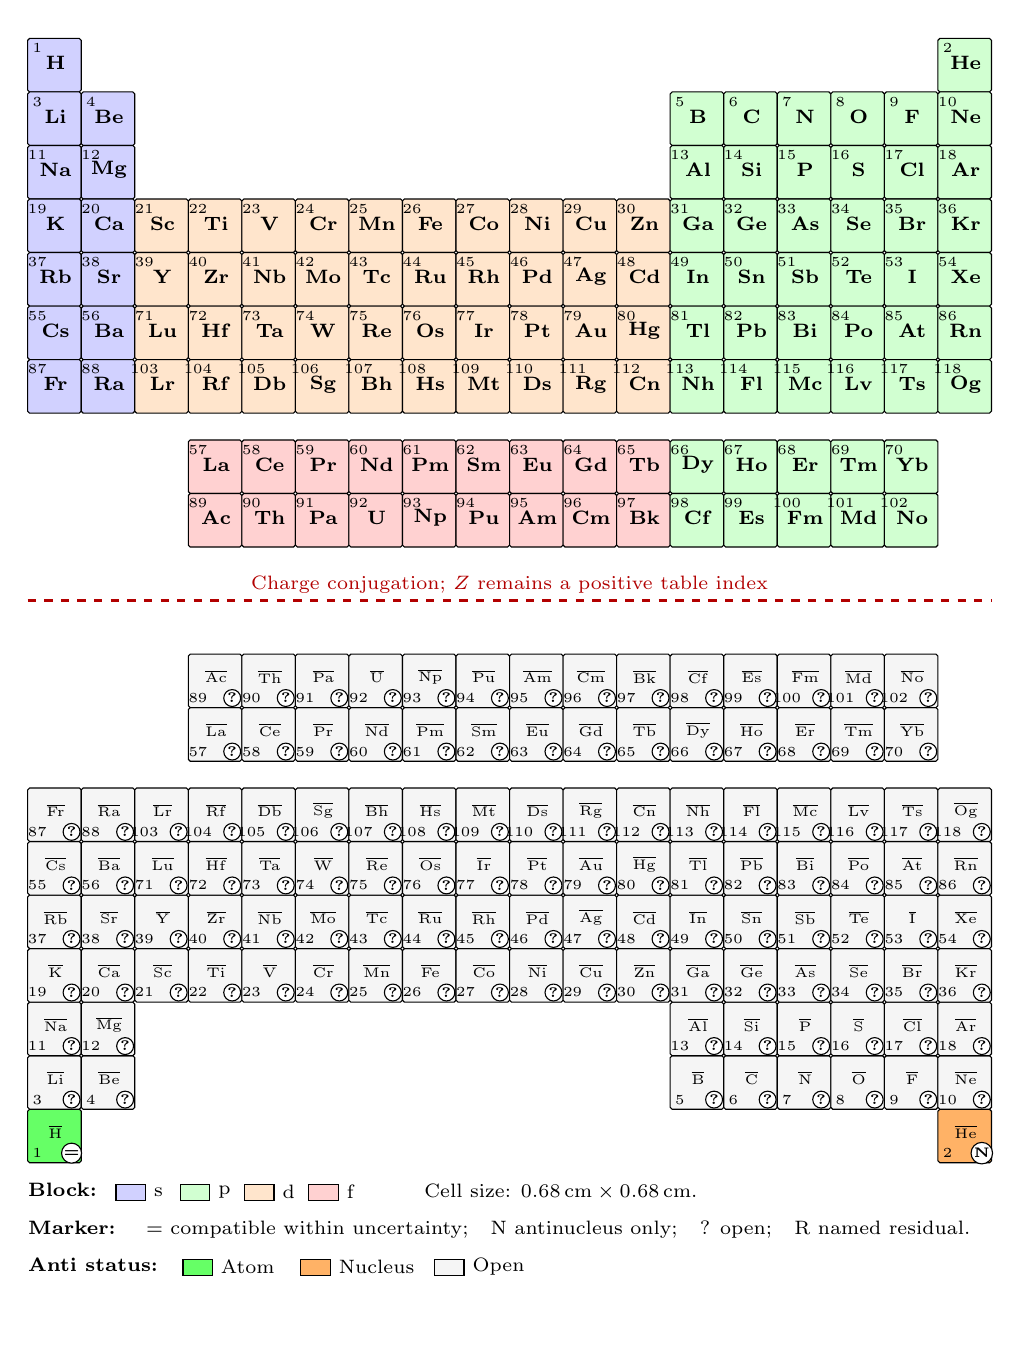
\begin{tikzpicture}[x=0.68cm, y=0.68cm, every node/.style={inner sep=0pt}]
\path[use as bounding box] (0,10.2) rectangle (18,-13.900000000000002);
\draw[fill=blue!18, draw=black, rounded corners=0.7pt] (0,10.0) rectangle (1,9.0);
\node at (0.52,9.54) {\scriptsize \textbf{H}};
\node at (0.18,9.82) {\tiny 1};
\draw[fill=green!18, draw=black, rounded corners=0.7pt] (17,10.0) rectangle (18,9.0);
\node at (17.52,9.54) {\scriptsize \textbf{He}};
\node at (17.18,9.82) {\tiny 2};
\draw[fill=blue!18, draw=black, rounded corners=0.7pt] (0,9.0) rectangle (1,8.0);
\node at (0.52,8.54) {\scriptsize \textbf{Li}};
\node at (0.18,8.82) {\tiny 3};
\draw[fill=blue!18, draw=black, rounded corners=0.7pt] (1,9.0) rectangle (2,8.0);
\node at (1.52,8.54) {\scriptsize \textbf{Be}};
\node at (1.18,8.82) {\tiny 4};
\draw[fill=green!18, draw=black, rounded corners=0.7pt] (12,9.0) rectangle (13,8.0);
\node at (12.52,8.54) {\scriptsize \textbf{B}};
\node at (12.18,8.82) {\tiny 5};
\draw[fill=green!18, draw=black, rounded corners=0.7pt] (13,9.0) rectangle (14,8.0);
\node at (13.52,8.54) {\scriptsize \textbf{C}};
\node at (13.18,8.82) {\tiny 6};
\draw[fill=green!18, draw=black, rounded corners=0.7pt] (14,9.0) rectangle (15,8.0);
\node at (14.52,8.54) {\scriptsize \textbf{N}};
\node at (14.18,8.82) {\tiny 7};
\draw[fill=green!18, draw=black, rounded corners=0.7pt] (15,9.0) rectangle (16,8.0);
\node at (15.52,8.54) {\scriptsize \textbf{O}};
\node at (15.18,8.82) {\tiny 8};
\draw[fill=green!18, draw=black, rounded corners=0.7pt] (16,9.0) rectangle (17,8.0);
\node at (16.52,8.54) {\scriptsize \textbf{F}};
\node at (16.18,8.82) {\tiny 9};
\draw[fill=green!18, draw=black, rounded corners=0.7pt] (17,9.0) rectangle (18,8.0);
\node at (17.52,8.54) {\scriptsize \textbf{Ne}};
\node at (17.18,8.82) {\tiny 10};
\draw[fill=blue!18, draw=black, rounded corners=0.7pt] (0,8.0) rectangle (1,7.0);
\node at (0.52,7.54) {\scriptsize \textbf{Na}};
\node at (0.18,7.82) {\tiny 11};
\draw[fill=blue!18, draw=black, rounded corners=0.7pt] (1,8.0) rectangle (2,7.0);
\node at (1.52,7.54) {\scriptsize \textbf{Mg}};
\node at (1.18,7.82) {\tiny 12};
\draw[fill=green!18, draw=black, rounded corners=0.7pt] (12,8.0) rectangle (13,7.0);
\node at (12.52,7.54) {\scriptsize \textbf{Al}};
\node at (12.18,7.82) {\tiny 13};
\draw[fill=green!18, draw=black, rounded corners=0.7pt] (13,8.0) rectangle (14,7.0);
\node at (13.52,7.54) {\scriptsize \textbf{Si}};
\node at (13.18,7.82) {\tiny 14};
\draw[fill=green!18, draw=black, rounded corners=0.7pt] (14,8.0) rectangle (15,7.0);
\node at (14.52,7.54) {\scriptsize \textbf{P}};
\node at (14.18,7.82) {\tiny 15};
\draw[fill=green!18, draw=black, rounded corners=0.7pt] (15,8.0) rectangle (16,7.0);
\node at (15.52,7.54) {\scriptsize \textbf{S}};
\node at (15.18,7.82) {\tiny 16};
\draw[fill=green!18, draw=black, rounded corners=0.7pt] (16,8.0) rectangle (17,7.0);
\node at (16.52,7.54) {\scriptsize \textbf{Cl}};
\node at (16.18,7.82) {\tiny 17};
\draw[fill=green!18, draw=black, rounded corners=0.7pt] (17,8.0) rectangle (18,7.0);
\node at (17.52,7.54) {\scriptsize \textbf{Ar}};
\node at (17.18,7.82) {\tiny 18};
\draw[fill=blue!18, draw=black, rounded corners=0.7pt] (0,7.0) rectangle (1,6.0);
\node at (0.52,6.54) {\scriptsize \textbf{K}};
\node at (0.18,6.82) {\tiny 19};
\draw[fill=blue!18, draw=black, rounded corners=0.7pt] (1,7.0) rectangle (2,6.0);
\node at (1.52,6.54) {\scriptsize \textbf{Ca}};
\node at (1.18,6.82) {\tiny 20};
\draw[fill=orange!20, draw=black, rounded corners=0.7pt] (2,7.0) rectangle (3,6.0);
\node at (2.52,6.54) {\scriptsize \textbf{Sc}};
\node at (2.18,6.82) {\tiny 21};
\draw[fill=orange!20, draw=black, rounded corners=0.7pt] (3,7.0) rectangle (4,6.0);
\node at (3.52,6.54) {\scriptsize \textbf{Ti}};
\node at (3.18,6.82) {\tiny 22};
\draw[fill=orange!20, draw=black, rounded corners=0.7pt] (4,7.0) rectangle (5,6.0);
\node at (4.52,6.54) {\scriptsize \textbf{V}};
\node at (4.18,6.82) {\tiny 23};
\draw[fill=orange!20, draw=black, rounded corners=0.7pt] (5,7.0) rectangle (6,6.0);
\node at (5.52,6.54) {\scriptsize \textbf{Cr}};
\node at (5.18,6.82) {\tiny 24};
\draw[fill=orange!20, draw=black, rounded corners=0.7pt] (6,7.0) rectangle (7,6.0);
\node at (6.52,6.54) {\scriptsize \textbf{Mn}};
\node at (6.18,6.82) {\tiny 25};
\draw[fill=orange!20, draw=black, rounded corners=0.7pt] (7,7.0) rectangle (8,6.0);
\node at (7.52,6.54) {\scriptsize \textbf{Fe}};
\node at (7.18,6.82) {\tiny 26};
\draw[fill=orange!20, draw=black, rounded corners=0.7pt] (8,7.0) rectangle (9,6.0);
\node at (8.52,6.54) {\scriptsize \textbf{Co}};
\node at (8.18,6.82) {\tiny 27};
\draw[fill=orange!20, draw=black, rounded corners=0.7pt] (9,7.0) rectangle (10,6.0);
\node at (9.52,6.54) {\scriptsize \textbf{Ni}};
\node at (9.18,6.82) {\tiny 28};
\draw[fill=orange!20, draw=black, rounded corners=0.7pt] (10,7.0) rectangle (11,6.0);
\node at (10.52,6.54) {\scriptsize \textbf{Cu}};
\node at (10.18,6.82) {\tiny 29};
\draw[fill=orange!20, draw=black, rounded corners=0.7pt] (11,7.0) rectangle (12,6.0);
\node at (11.52,6.54) {\scriptsize \textbf{Zn}};
\node at (11.18,6.82) {\tiny 30};
\draw[fill=green!18, draw=black, rounded corners=0.7pt] (12,7.0) rectangle (13,6.0);
\node at (12.52,6.54) {\scriptsize \textbf{Ga}};
\node at (12.18,6.82) {\tiny 31};
\draw[fill=green!18, draw=black, rounded corners=0.7pt] (13,7.0) rectangle (14,6.0);
\node at (13.52,6.54) {\scriptsize \textbf{Ge}};
\node at (13.18,6.82) {\tiny 32};
\draw[fill=green!18, draw=black, rounded corners=0.7pt] (14,7.0) rectangle (15,6.0);
\node at (14.52,6.54) {\scriptsize \textbf{As}};
\node at (14.18,6.82) {\tiny 33};
\draw[fill=green!18, draw=black, rounded corners=0.7pt] (15,7.0) rectangle (16,6.0);
\node at (15.52,6.54) {\scriptsize \textbf{Se}};
\node at (15.18,6.82) {\tiny 34};
\draw[fill=green!18, draw=black, rounded corners=0.7pt] (16,7.0) rectangle (17,6.0);
\node at (16.52,6.54) {\scriptsize \textbf{Br}};
\node at (16.18,6.82) {\tiny 35};
\draw[fill=green!18, draw=black, rounded corners=0.7pt] (17,7.0) rectangle (18,6.0);
\node at (17.52,6.54) {\scriptsize \textbf{Kr}};
\node at (17.18,6.82) {\tiny 36};
\draw[fill=blue!18, draw=black, rounded corners=0.7pt] (0,6.0) rectangle (1,5.0);
\node at (0.52,5.54) {\scriptsize \textbf{Rb}};
\node at (0.18,5.82) {\tiny 37};
\draw[fill=blue!18, draw=black, rounded corners=0.7pt] (1,6.0) rectangle (2,5.0);
\node at (1.52,5.54) {\scriptsize \textbf{Sr}};
\node at (1.18,5.82) {\tiny 38};
\draw[fill=orange!20, draw=black, rounded corners=0.7pt] (2,6.0) rectangle (3,5.0);
\node at (2.52,5.54) {\scriptsize \textbf{Y}};
\node at (2.18,5.82) {\tiny 39};
\draw[fill=orange!20, draw=black, rounded corners=0.7pt] (3,6.0) rectangle (4,5.0);
\node at (3.52,5.54) {\scriptsize \textbf{Zr}};
\node at (3.18,5.82) {\tiny 40};
\draw[fill=orange!20, draw=black, rounded corners=0.7pt] (4,6.0) rectangle (5,5.0);
\node at (4.52,5.54) {\scriptsize \textbf{Nb}};
\node at (4.18,5.82) {\tiny 41};
\draw[fill=orange!20, draw=black, rounded corners=0.7pt] (5,6.0) rectangle (6,5.0);
\node at (5.52,5.54) {\scriptsize \textbf{Mo}};
\node at (5.18,5.82) {\tiny 42};
\draw[fill=orange!20, draw=black, rounded corners=0.7pt] (6,6.0) rectangle (7,5.0);
\node at (6.52,5.54) {\scriptsize \textbf{Tc}};
\node at (6.18,5.82) {\tiny 43};
\draw[fill=orange!20, draw=black, rounded corners=0.7pt] (7,6.0) rectangle (8,5.0);
\node at (7.52,5.54) {\scriptsize \textbf{Ru}};
\node at (7.18,5.82) {\tiny 44};
\draw[fill=orange!20, draw=black, rounded corners=0.7pt] (8,6.0) rectangle (9,5.0);
\node at (8.52,5.54) {\scriptsize \textbf{Rh}};
\node at (8.18,5.82) {\tiny 45};
\draw[fill=orange!20, draw=black, rounded corners=0.7pt] (9,6.0) rectangle (10,5.0);
\node at (9.52,5.54) {\scriptsize \textbf{Pd}};
\node at (9.18,5.82) {\tiny 46};
\draw[fill=orange!20, draw=black, rounded corners=0.7pt] (10,6.0) rectangle (11,5.0);
\node at (10.52,5.54) {\scriptsize \textbf{Ag}};
\node at (10.18,5.82) {\tiny 47};
\draw[fill=orange!20, draw=black, rounded corners=0.7pt] (11,6.0) rectangle (12,5.0);
\node at (11.52,5.54) {\scriptsize \textbf{Cd}};
\node at (11.18,5.82) {\tiny 48};
\draw[fill=green!18, draw=black, rounded corners=0.7pt] (12,6.0) rectangle (13,5.0);
\node at (12.52,5.54) {\scriptsize \textbf{In}};
\node at (12.18,5.82) {\tiny 49};
\draw[fill=green!18, draw=black, rounded corners=0.7pt] (13,6.0) rectangle (14,5.0);
\node at (13.52,5.54) {\scriptsize \textbf{Sn}};
\node at (13.18,5.82) {\tiny 50};
\draw[fill=green!18, draw=black, rounded corners=0.7pt] (14,6.0) rectangle (15,5.0);
\node at (14.52,5.54) {\scriptsize \textbf{Sb}};
\node at (14.18,5.82) {\tiny 51};
\draw[fill=green!18, draw=black, rounded corners=0.7pt] (15,6.0) rectangle (16,5.0);
\node at (15.52,5.54) {\scriptsize \textbf{Te}};
\node at (15.18,5.82) {\tiny 52};
\draw[fill=green!18, draw=black, rounded corners=0.7pt] (16,6.0) rectangle (17,5.0);
\node at (16.52,5.54) {\scriptsize \textbf{I}};
\node at (16.18,5.82) {\tiny 53};
\draw[fill=green!18, draw=black, rounded corners=0.7pt] (17,6.0) rectangle (18,5.0);
\node at (17.52,5.54) {\scriptsize \textbf{Xe}};
\node at (17.18,5.82) {\tiny 54};
\draw[fill=blue!18, draw=black, rounded corners=0.7pt] (0,5.0) rectangle (1,4.0);
\node at (0.52,4.54) {\scriptsize \textbf{Cs}};
\node at (0.18,4.82) {\tiny 55};
\draw[fill=blue!18, draw=black, rounded corners=0.7pt] (1,5.0) rectangle (2,4.0);
\node at (1.52,4.54) {\scriptsize \textbf{Ba}};
\node at (1.18,4.82) {\tiny 56};
\draw[fill=orange!20, draw=black, rounded corners=0.7pt] (2,5.0) rectangle (3,4.0);
\node at (2.52,4.54) {\scriptsize \textbf{Lu}};
\node at (2.18,4.82) {\tiny 71};
\draw[fill=orange!20, draw=black, rounded corners=0.7pt] (3,5.0) rectangle (4,4.0);
\node at (3.52,4.54) {\scriptsize \textbf{Hf}};
\node at (3.18,4.82) {\tiny 72};
\draw[fill=orange!20, draw=black, rounded corners=0.7pt] (4,5.0) rectangle (5,4.0);
\node at (4.52,4.54) {\scriptsize \textbf{Ta}};
\node at (4.18,4.82) {\tiny 73};
\draw[fill=orange!20, draw=black, rounded corners=0.7pt] (5,5.0) rectangle (6,4.0);
\node at (5.52,4.54) {\scriptsize \textbf{W}};
\node at (5.18,4.82) {\tiny 74};
\draw[fill=orange!20, draw=black, rounded corners=0.7pt] (6,5.0) rectangle (7,4.0);
\node at (6.52,4.54) {\scriptsize \textbf{Re}};
\node at (6.18,4.82) {\tiny 75};
\draw[fill=orange!20, draw=black, rounded corners=0.7pt] (7,5.0) rectangle (8,4.0);
\node at (7.52,4.54) {\scriptsize \textbf{Os}};
\node at (7.18,4.82) {\tiny 76};
\draw[fill=orange!20, draw=black, rounded corners=0.7pt] (8,5.0) rectangle (9,4.0);
\node at (8.52,4.54) {\scriptsize \textbf{Ir}};
\node at (8.18,4.82) {\tiny 77};
\draw[fill=orange!20, draw=black, rounded corners=0.7pt] (9,5.0) rectangle (10,4.0);
\node at (9.52,4.54) {\scriptsize \textbf{Pt}};
\node at (9.18,4.82) {\tiny 78};
\draw[fill=orange!20, draw=black, rounded corners=0.7pt] (10,5.0) rectangle (11,4.0);
\node at (10.52,4.54) {\scriptsize \textbf{Au}};
\node at (10.18,4.82) {\tiny 79};
\draw[fill=orange!20, draw=black, rounded corners=0.7pt] (11,5.0) rectangle (12,4.0);
\node at (11.52,4.54) {\scriptsize \textbf{Hg}};
\node at (11.18,4.82) {\tiny 80};
\draw[fill=green!18, draw=black, rounded corners=0.7pt] (12,5.0) rectangle (13,4.0);
\node at (12.52,4.54) {\scriptsize \textbf{Tl}};
\node at (12.18,4.82) {\tiny 81};
\draw[fill=green!18, draw=black, rounded corners=0.7pt] (13,5.0) rectangle (14,4.0);
\node at (13.52,4.54) {\scriptsize \textbf{Pb}};
\node at (13.18,4.82) {\tiny 82};
\draw[fill=green!18, draw=black, rounded corners=0.7pt] (14,5.0) rectangle (15,4.0);
\node at (14.52,4.54) {\scriptsize \textbf{Bi}};
\node at (14.18,4.82) {\tiny 83};
\draw[fill=green!18, draw=black, rounded corners=0.7pt] (15,5.0) rectangle (16,4.0);
\node at (15.52,4.54) {\scriptsize \textbf{Po}};
\node at (15.18,4.82) {\tiny 84};
\draw[fill=green!18, draw=black, rounded corners=0.7pt] (16,5.0) rectangle (17,4.0);
\node at (16.52,4.54) {\scriptsize \textbf{At}};
\node at (16.18,4.82) {\tiny 85};
\draw[fill=green!18, draw=black, rounded corners=0.7pt] (17,5.0) rectangle (18,4.0);
\node at (17.52,4.54) {\scriptsize \textbf{Rn}};
\node at (17.18,4.82) {\tiny 86};
\draw[fill=blue!18, draw=black, rounded corners=0.7pt] (0,4.0) rectangle (1,3.0);
\node at (0.52,3.54) {\scriptsize \textbf{Fr}};
\node at (0.18,3.82) {\tiny 87};
\draw[fill=blue!18, draw=black, rounded corners=0.7pt] (1,4.0) rectangle (2,3.0);
\node at (1.52,3.54) {\scriptsize \textbf{Ra}};
\node at (1.18,3.82) {\tiny 88};
\draw[fill=orange!20, draw=black, rounded corners=0.7pt] (2,4.0) rectangle (3,3.0);
\node at (2.52,3.54) {\scriptsize \textbf{Lr}};
\node at (2.18,3.82) {\tiny 103};
\draw[fill=orange!20, draw=black, rounded corners=0.7pt] (3,4.0) rectangle (4,3.0);
\node at (3.52,3.54) {\scriptsize \textbf{Rf}};
\node at (3.18,3.82) {\tiny 104};
\draw[fill=orange!20, draw=black, rounded corners=0.7pt] (4,4.0) rectangle (5,3.0);
\node at (4.52,3.54) {\scriptsize \textbf{Db}};
\node at (4.18,3.82) {\tiny 105};
\draw[fill=orange!20, draw=black, rounded corners=0.7pt] (5,4.0) rectangle (6,3.0);
\node at (5.52,3.54) {\scriptsize \textbf{Sg}};
\node at (5.18,3.82) {\tiny 106};
\draw[fill=orange!20, draw=black, rounded corners=0.7pt] (6,4.0) rectangle (7,3.0);
\node at (6.52,3.54) {\scriptsize \textbf{Bh}};
\node at (6.18,3.82) {\tiny 107};
\draw[fill=orange!20, draw=black, rounded corners=0.7pt] (7,4.0) rectangle (8,3.0);
\node at (7.52,3.54) {\scriptsize \textbf{Hs}};
\node at (7.18,3.82) {\tiny 108};
\draw[fill=orange!20, draw=black, rounded corners=0.7pt] (8,4.0) rectangle (9,3.0);
\node at (8.52,3.54) {\scriptsize \textbf{Mt}};
\node at (8.18,3.82) {\tiny 109};
\draw[fill=orange!20, draw=black, rounded corners=0.7pt] (9,4.0) rectangle (10,3.0);
\node at (9.52,3.54) {\scriptsize \textbf{Ds}};
\node at (9.18,3.82) {\tiny 110};
\draw[fill=orange!20, draw=black, rounded corners=0.7pt] (10,4.0) rectangle (11,3.0);
\node at (10.52,3.54) {\scriptsize \textbf{Rg}};
\node at (10.18,3.82) {\tiny 111};
\draw[fill=orange!20, draw=black, rounded corners=0.7pt] (11,4.0) rectangle (12,3.0);
\node at (11.52,3.54) {\scriptsize \textbf{Cn}};
\node at (11.18,3.82) {\tiny 112};
\draw[fill=green!18, draw=black, rounded corners=0.7pt] (12,4.0) rectangle (13,3.0);
\node at (12.52,3.54) {\scriptsize \textbf{Nh}};
\node at (12.18,3.82) {\tiny 113};
\draw[fill=green!18, draw=black, rounded corners=0.7pt] (13,4.0) rectangle (14,3.0);
\node at (13.52,3.54) {\scriptsize \textbf{Fl}};
\node at (13.18,3.82) {\tiny 114};
\draw[fill=green!18, draw=black, rounded corners=0.7pt] (14,4.0) rectangle (15,3.0);
\node at (14.52,3.54) {\scriptsize \textbf{Mc}};
\node at (14.18,3.82) {\tiny 115};
\draw[fill=green!18, draw=black, rounded corners=0.7pt] (15,4.0) rectangle (16,3.0);
\node at (15.52,3.54) {\scriptsize \textbf{Lv}};
\node at (15.18,3.82) {\tiny 116};
\draw[fill=green!18, draw=black, rounded corners=0.7pt] (16,4.0) rectangle (17,3.0);
\node at (16.52,3.54) {\scriptsize \textbf{Ts}};
\node at (16.18,3.82) {\tiny 117};
\draw[fill=green!18, draw=black, rounded corners=0.7pt] (17,4.0) rectangle (18,3.0);
\node at (17.52,3.54) {\scriptsize \textbf{Og}};
\node at (17.18,3.82) {\tiny 118};
\draw[fill=red!18, draw=black, rounded corners=0.7pt] (3,2.5) rectangle (4,1.5);
\node at (3.52,2.04) {\scriptsize \textbf{La}};
\node at (3.18,2.32) {\tiny 57};
\draw[fill=red!18, draw=black, rounded corners=0.7pt] (4,2.5) rectangle (5,1.5);
\node at (4.52,2.04) {\scriptsize \textbf{Ce}};
\node at (4.18,2.32) {\tiny 58};
\draw[fill=red!18, draw=black, rounded corners=0.7pt] (5,2.5) rectangle (6,1.5);
\node at (5.52,2.04) {\scriptsize \textbf{Pr}};
\node at (5.18,2.32) {\tiny 59};
\draw[fill=red!18, draw=black, rounded corners=0.7pt] (6,2.5) rectangle (7,1.5);
\node at (6.52,2.04) {\scriptsize \textbf{Nd}};
\node at (6.18,2.32) {\tiny 60};
\draw[fill=red!18, draw=black, rounded corners=0.7pt] (7,2.5) rectangle (8,1.5);
\node at (7.52,2.04) {\scriptsize \textbf{Pm}};
\node at (7.18,2.32) {\tiny 61};
\draw[fill=red!18, draw=black, rounded corners=0.7pt] (8,2.5) rectangle (9,1.5);
\node at (8.52,2.04) {\scriptsize \textbf{Sm}};
\node at (8.18,2.32) {\tiny 62};
\draw[fill=red!18, draw=black, rounded corners=0.7pt] (9,2.5) rectangle (10,1.5);
\node at (9.52,2.04) {\scriptsize \textbf{Eu}};
\node at (9.18,2.32) {\tiny 63};
\draw[fill=red!18, draw=black, rounded corners=0.7pt] (10,2.5) rectangle (11,1.5);
\node at (10.52,2.04) {\scriptsize \textbf{Gd}};
\node at (10.18,2.32) {\tiny 64};
\draw[fill=red!18, draw=black, rounded corners=0.7pt] (11,2.5) rectangle (12,1.5);
\node at (11.52,2.04) {\scriptsize \textbf{Tb}};
\node at (11.18,2.32) {\tiny 65};
\draw[fill=green!18, draw=black, rounded corners=0.7pt] (12,2.5) rectangle (13,1.5);
\node at (12.52,2.04) {\scriptsize \textbf{Dy}};
\node at (12.18,2.32) {\tiny 66};
\draw[fill=green!18, draw=black, rounded corners=0.7pt] (13,2.5) rectangle (14,1.5);
\node at (13.52,2.04) {\scriptsize \textbf{Ho}};
\node at (13.18,2.32) {\tiny 67};
\draw[fill=green!18, draw=black, rounded corners=0.7pt] (14,2.5) rectangle (15,1.5);
\node at (14.52,2.04) {\scriptsize \textbf{Er}};
\node at (14.18,2.32) {\tiny 68};
\draw[fill=green!18, draw=black, rounded corners=0.7pt] (15,2.5) rectangle (16,1.5);
\node at (15.52,2.04) {\scriptsize \textbf{Tm}};
\node at (15.18,2.32) {\tiny 69};
\draw[fill=green!18, draw=black, rounded corners=0.7pt] (16,2.5) rectangle (17,1.5);
\node at (16.52,2.04) {\scriptsize \textbf{Yb}};
\node at (16.18,2.32) {\tiny 70};
\draw[fill=red!18, draw=black, rounded corners=0.7pt] (3,1.5) rectangle (4,0.5);
\node at (3.52,1.04) {\scriptsize \textbf{Ac}};
\node at (3.18,1.32) {\tiny 89};
\draw[fill=red!18, draw=black, rounded corners=0.7pt] (4,1.5) rectangle (5,0.5);
\node at (4.52,1.04) {\scriptsize \textbf{Th}};
\node at (4.18,1.32) {\tiny 90};
\draw[fill=red!18, draw=black, rounded corners=0.7pt] (5,1.5) rectangle (6,0.5);
\node at (5.52,1.04) {\scriptsize \textbf{Pa}};
\node at (5.18,1.32) {\tiny 91};
\draw[fill=red!18, draw=black, rounded corners=0.7pt] (6,1.5) rectangle (7,0.5);
\node at (6.52,1.04) {\scriptsize \textbf{U}};
\node at (6.18,1.32) {\tiny 92};
\draw[fill=red!18, draw=black, rounded corners=0.7pt] (7,1.5) rectangle (8,0.5);
\node at (7.52,1.04) {\scriptsize \textbf{Np}};
\node at (7.18,1.32) {\tiny 93};
\draw[fill=red!18, draw=black, rounded corners=0.7pt] (8,1.5) rectangle (9,0.5);
\node at (8.52,1.04) {\scriptsize \textbf{Pu}};
\node at (8.18,1.32) {\tiny 94};
\draw[fill=red!18, draw=black, rounded corners=0.7pt] (9,1.5) rectangle (10,0.5);
\node at (9.52,1.04) {\scriptsize \textbf{Am}};
\node at (9.18,1.32) {\tiny 95};
\draw[fill=red!18, draw=black, rounded corners=0.7pt] (10,1.5) rectangle (11,0.5);
\node at (10.52,1.04) {\scriptsize \textbf{Cm}};
\node at (10.18,1.32) {\tiny 96};
\draw[fill=red!18, draw=black, rounded corners=0.7pt] (11,1.5) rectangle (12,0.5);
\node at (11.52,1.04) {\scriptsize \textbf{Bk}};
\node at (11.18,1.32) {\tiny 97};
\draw[fill=green!18, draw=black, rounded corners=0.7pt] (12,1.5) rectangle (13,0.5);
\node at (12.52,1.04) {\scriptsize \textbf{Cf}};
\node at (12.18,1.32) {\tiny 98};
\draw[fill=green!18, draw=black, rounded corners=0.7pt] (13,1.5) rectangle (14,0.5);
\node at (13.52,1.04) {\scriptsize \textbf{Es}};
\node at (13.18,1.32) {\tiny 99};
\draw[fill=green!18, draw=black, rounded corners=0.7pt] (14,1.5) rectangle (15,0.5);
\node at (14.52,1.04) {\scriptsize \textbf{Fm}};
\node at (14.18,1.32) {\tiny 100};
\draw[fill=green!18, draw=black, rounded corners=0.7pt] (15,1.5) rectangle (16,0.5);
\node at (15.52,1.04) {\scriptsize \textbf{Md}};
\node at (15.18,1.32) {\tiny 101};
\draw[fill=green!18, draw=black, rounded corners=0.7pt] (16,1.5) rectangle (17,0.5);
\node at (16.52,1.04) {\scriptsize \textbf{No}};
\node at (16.18,1.32) {\tiny 102};
\draw[line width=1.2pt, dashed, red!70!black] (0,-0.5) -- (18,-0.5) node[midway, above=2pt, text=red!70!black] {\scriptsize Charge conjugation; $Z$ remains a positive table index};
\draw[fill=green!60, draw=black, rounded corners=0.7pt] (0,-10.0) rectangle (1,-11.0);
\node at (0.52,-10.42) {\tiny \textbf{$\overline{\mathrm{H}}$}};
\node at (0.18,-10.82) {\tiny 1};
\node[fill=white, draw=black, circle, inner sep=0.4pt] at (0.82,-10.82) {\tiny \textbf{=}};
\draw[fill=orange!60, draw=black, rounded corners=0.7pt] (17,-10.0) rectangle (18,-11.0);
\node at (17.52,-10.42) {\tiny \textbf{$\overline{\mathrm{He}}$}};
\node at (17.18,-10.82) {\tiny 2};
\node[fill=white, draw=black, circle, inner sep=0.4pt] at (17.82,-10.82) {\tiny \textbf{N}};
\draw[fill=gray!8, draw=black, rounded corners=0.7pt] (0,-9.0) rectangle (1,-10.0);
\node at (0.52,-9.42) {\tiny \textbf{$\overline{\mathrm{Li}}$}};
\node at (0.18,-9.82) {\tiny 3};
\node[fill=white, draw=black, circle, inner sep=0.4pt] at (0.82,-9.82) {\tiny \textbf{?}};
\draw[fill=gray!8, draw=black, rounded corners=0.7pt] (1,-9.0) rectangle (2,-10.0);
\node at (1.52,-9.42) {\tiny \textbf{$\overline{\mathrm{Be}}$}};
\node at (1.18,-9.82) {\tiny 4};
\node[fill=white, draw=black, circle, inner sep=0.4pt] at (1.8199999999999998,-9.82) {\tiny \textbf{?}};
\draw[fill=gray!8, draw=black, rounded corners=0.7pt] (12,-9.0) rectangle (13,-10.0);
\node at (12.52,-9.42) {\tiny \textbf{$\overline{\mathrm{B}}$}};
\node at (12.18,-9.82) {\tiny 5};
\node[fill=white, draw=black, circle, inner sep=0.4pt] at (12.82,-9.82) {\tiny \textbf{?}};
\draw[fill=gray!8, draw=black, rounded corners=0.7pt] (13,-9.0) rectangle (14,-10.0);
\node at (13.52,-9.42) {\tiny \textbf{$\overline{\mathrm{C}}$}};
\node at (13.18,-9.82) {\tiny 6};
\node[fill=white, draw=black, circle, inner sep=0.4pt] at (13.82,-9.82) {\tiny \textbf{?}};
\draw[fill=gray!8, draw=black, rounded corners=0.7pt] (14,-9.0) rectangle (15,-10.0);
\node at (14.52,-9.42) {\tiny \textbf{$\overline{\mathrm{N}}$}};
\node at (14.18,-9.82) {\tiny 7};
\node[fill=white, draw=black, circle, inner sep=0.4pt] at (14.82,-9.82) {\tiny \textbf{?}};
\draw[fill=gray!8, draw=black, rounded corners=0.7pt] (15,-9.0) rectangle (16,-10.0);
\node at (15.52,-9.42) {\tiny \textbf{$\overline{\mathrm{O}}$}};
\node at (15.18,-9.82) {\tiny 8};
\node[fill=white, draw=black, circle, inner sep=0.4pt] at (15.82,-9.82) {\tiny \textbf{?}};
\draw[fill=gray!8, draw=black, rounded corners=0.7pt] (16,-9.0) rectangle (17,-10.0);
\node at (16.52,-9.42) {\tiny \textbf{$\overline{\mathrm{F}}$}};
\node at (16.18,-9.82) {\tiny 9};
\node[fill=white, draw=black, circle, inner sep=0.4pt] at (16.82,-9.82) {\tiny \textbf{?}};
\draw[fill=gray!8, draw=black, rounded corners=0.7pt] (17,-9.0) rectangle (18,-10.0);
\node at (17.52,-9.42) {\tiny \textbf{$\overline{\mathrm{Ne}}$}};
\node at (17.18,-9.82) {\tiny 10};
\node[fill=white, draw=black, circle, inner sep=0.4pt] at (17.82,-9.82) {\tiny \textbf{?}};
\draw[fill=gray!8, draw=black, rounded corners=0.7pt] (0,-8.0) rectangle (1,-9.0);
\node at (0.52,-8.42) {\tiny \textbf{$\overline{\mathrm{Na}}$}};
\node at (0.18,-8.82) {\tiny 11};
\node[fill=white, draw=black, circle, inner sep=0.4pt] at (0.82,-8.82) {\tiny \textbf{?}};
\draw[fill=gray!8, draw=black, rounded corners=0.7pt] (1,-8.0) rectangle (2,-9.0);
\node at (1.52,-8.42) {\tiny \textbf{$\overline{\mathrm{Mg}}$}};
\node at (1.18,-8.82) {\tiny 12};
\node[fill=white, draw=black, circle, inner sep=0.4pt] at (1.8199999999999998,-8.82) {\tiny \textbf{?}};
\draw[fill=gray!8, draw=black, rounded corners=0.7pt] (12,-8.0) rectangle (13,-9.0);
\node at (12.52,-8.42) {\tiny \textbf{$\overline{\mathrm{Al}}$}};
\node at (12.18,-8.82) {\tiny 13};
\node[fill=white, draw=black, circle, inner sep=0.4pt] at (12.82,-8.82) {\tiny \textbf{?}};
\draw[fill=gray!8, draw=black, rounded corners=0.7pt] (13,-8.0) rectangle (14,-9.0);
\node at (13.52,-8.42) {\tiny \textbf{$\overline{\mathrm{Si}}$}};
\node at (13.18,-8.82) {\tiny 14};
\node[fill=white, draw=black, circle, inner sep=0.4pt] at (13.82,-8.82) {\tiny \textbf{?}};
\draw[fill=gray!8, draw=black, rounded corners=0.7pt] (14,-8.0) rectangle (15,-9.0);
\node at (14.52,-8.42) {\tiny \textbf{$\overline{\mathrm{P}}$}};
\node at (14.18,-8.82) {\tiny 15};
\node[fill=white, draw=black, circle, inner sep=0.4pt] at (14.82,-8.82) {\tiny \textbf{?}};
\draw[fill=gray!8, draw=black, rounded corners=0.7pt] (15,-8.0) rectangle (16,-9.0);
\node at (15.52,-8.42) {\tiny \textbf{$\overline{\mathrm{S}}$}};
\node at (15.18,-8.82) {\tiny 16};
\node[fill=white, draw=black, circle, inner sep=0.4pt] at (15.82,-8.82) {\tiny \textbf{?}};
\draw[fill=gray!8, draw=black, rounded corners=0.7pt] (16,-8.0) rectangle (17,-9.0);
\node at (16.52,-8.42) {\tiny \textbf{$\overline{\mathrm{Cl}}$}};
\node at (16.18,-8.82) {\tiny 17};
\node[fill=white, draw=black, circle, inner sep=0.4pt] at (16.82,-8.82) {\tiny \textbf{?}};
\draw[fill=gray!8, draw=black, rounded corners=0.7pt] (17,-8.0) rectangle (18,-9.0);
\node at (17.52,-8.42) {\tiny \textbf{$\overline{\mathrm{Ar}}$}};
\node at (17.18,-8.82) {\tiny 18};
\node[fill=white, draw=black, circle, inner sep=0.4pt] at (17.82,-8.82) {\tiny \textbf{?}};
\draw[fill=gray!8, draw=black, rounded corners=0.7pt] (0,-7.0) rectangle (1,-8.0);
\node at (0.52,-7.42) {\tiny \textbf{$\overline{\mathrm{K}}$}};
\node at (0.18,-7.82) {\tiny 19};
\node[fill=white, draw=black, circle, inner sep=0.4pt] at (0.82,-7.82) {\tiny \textbf{?}};
\draw[fill=gray!8, draw=black, rounded corners=0.7pt] (1,-7.0) rectangle (2,-8.0);
\node at (1.52,-7.42) {\tiny \textbf{$\overline{\mathrm{Ca}}$}};
\node at (1.18,-7.82) {\tiny 20};
\node[fill=white, draw=black, circle, inner sep=0.4pt] at (1.8199999999999998,-7.82) {\tiny \textbf{?}};
\draw[fill=gray!8, draw=black, rounded corners=0.7pt] (2,-7.0) rectangle (3,-8.0);
\node at (2.52,-7.42) {\tiny \textbf{$\overline{\mathrm{Sc}}$}};
\node at (2.18,-7.82) {\tiny 21};
\node[fill=white, draw=black, circle, inner sep=0.4pt] at (2.82,-7.82) {\tiny \textbf{?}};
\draw[fill=gray!8, draw=black, rounded corners=0.7pt] (3,-7.0) rectangle (4,-8.0);
\node at (3.52,-7.42) {\tiny \textbf{$\overline{\mathrm{Ti}}$}};
\node at (3.18,-7.82) {\tiny 22};
\node[fill=white, draw=black, circle, inner sep=0.4pt] at (3.82,-7.82) {\tiny \textbf{?}};
\draw[fill=gray!8, draw=black, rounded corners=0.7pt] (4,-7.0) rectangle (5,-8.0);
\node at (4.52,-7.42) {\tiny \textbf{$\overline{\mathrm{V}}$}};
\node at (4.18,-7.82) {\tiny 23};
\node[fill=white, draw=black, circle, inner sep=0.4pt] at (4.82,-7.82) {\tiny \textbf{?}};
\draw[fill=gray!8, draw=black, rounded corners=0.7pt] (5,-7.0) rectangle (6,-8.0);
\node at (5.52,-7.42) {\tiny \textbf{$\overline{\mathrm{Cr}}$}};
\node at (5.18,-7.82) {\tiny 24};
\node[fill=white, draw=black, circle, inner sep=0.4pt] at (5.82,-7.82) {\tiny \textbf{?}};
\draw[fill=gray!8, draw=black, rounded corners=0.7pt] (6,-7.0) rectangle (7,-8.0);
\node at (6.52,-7.42) {\tiny \textbf{$\overline{\mathrm{Mn}}$}};
\node at (6.18,-7.82) {\tiny 25};
\node[fill=white, draw=black, circle, inner sep=0.4pt] at (6.82,-7.82) {\tiny \textbf{?}};
\draw[fill=gray!8, draw=black, rounded corners=0.7pt] (7,-7.0) rectangle (8,-8.0);
\node at (7.52,-7.42) {\tiny \textbf{$\overline{\mathrm{Fe}}$}};
\node at (7.18,-7.82) {\tiny 26};
\node[fill=white, draw=black, circle, inner sep=0.4pt] at (7.82,-7.82) {\tiny \textbf{?}};
\draw[fill=gray!8, draw=black, rounded corners=0.7pt] (8,-7.0) rectangle (9,-8.0);
\node at (8.52,-7.42) {\tiny \textbf{$\overline{\mathrm{Co}}$}};
\node at (8.18,-7.82) {\tiny 27};
\node[fill=white, draw=black, circle, inner sep=0.4pt] at (8.82,-7.82) {\tiny \textbf{?}};
\draw[fill=gray!8, draw=black, rounded corners=0.7pt] (9,-7.0) rectangle (10,-8.0);
\node at (9.52,-7.42) {\tiny \textbf{$\overline{\mathrm{Ni}}$}};
\node at (9.18,-7.82) {\tiny 28};
\node[fill=white, draw=black, circle, inner sep=0.4pt] at (9.82,-7.82) {\tiny \textbf{?}};
\draw[fill=gray!8, draw=black, rounded corners=0.7pt] (10,-7.0) rectangle (11,-8.0);
\node at (10.52,-7.42) {\tiny \textbf{$\overline{\mathrm{Cu}}$}};
\node at (10.18,-7.82) {\tiny 29};
\node[fill=white, draw=black, circle, inner sep=0.4pt] at (10.82,-7.82) {\tiny \textbf{?}};
\draw[fill=gray!8, draw=black, rounded corners=0.7pt] (11,-7.0) rectangle (12,-8.0);
\node at (11.52,-7.42) {\tiny \textbf{$\overline{\mathrm{Zn}}$}};
\node at (11.18,-7.82) {\tiny 30};
\node[fill=white, draw=black, circle, inner sep=0.4pt] at (11.82,-7.82) {\tiny \textbf{?}};
\draw[fill=gray!8, draw=black, rounded corners=0.7pt] (12,-7.0) rectangle (13,-8.0);
\node at (12.52,-7.42) {\tiny \textbf{$\overline{\mathrm{Ga}}$}};
\node at (12.18,-7.82) {\tiny 31};
\node[fill=white, draw=black, circle, inner sep=0.4pt] at (12.82,-7.82) {\tiny \textbf{?}};
\draw[fill=gray!8, draw=black, rounded corners=0.7pt] (13,-7.0) rectangle (14,-8.0);
\node at (13.52,-7.42) {\tiny \textbf{$\overline{\mathrm{Ge}}$}};
\node at (13.18,-7.82) {\tiny 32};
\node[fill=white, draw=black, circle, inner sep=0.4pt] at (13.82,-7.82) {\tiny \textbf{?}};
\draw[fill=gray!8, draw=black, rounded corners=0.7pt] (14,-7.0) rectangle (15,-8.0);
\node at (14.52,-7.42) {\tiny \textbf{$\overline{\mathrm{As}}$}};
\node at (14.18,-7.82) {\tiny 33};
\node[fill=white, draw=black, circle, inner sep=0.4pt] at (14.82,-7.82) {\tiny \textbf{?}};
\draw[fill=gray!8, draw=black, rounded corners=0.7pt] (15,-7.0) rectangle (16,-8.0);
\node at (15.52,-7.42) {\tiny \textbf{$\overline{\mathrm{Se}}$}};
\node at (15.18,-7.82) {\tiny 34};
\node[fill=white, draw=black, circle, inner sep=0.4pt] at (15.82,-7.82) {\tiny \textbf{?}};
\draw[fill=gray!8, draw=black, rounded corners=0.7pt] (16,-7.0) rectangle (17,-8.0);
\node at (16.52,-7.42) {\tiny \textbf{$\overline{\mathrm{Br}}$}};
\node at (16.18,-7.82) {\tiny 35};
\node[fill=white, draw=black, circle, inner sep=0.4pt] at (16.82,-7.82) {\tiny \textbf{?}};
\draw[fill=gray!8, draw=black, rounded corners=0.7pt] (17,-7.0) rectangle (18,-8.0);
\node at (17.52,-7.42) {\tiny \textbf{$\overline{\mathrm{Kr}}$}};
\node at (17.18,-7.82) {\tiny 36};
\node[fill=white, draw=black, circle, inner sep=0.4pt] at (17.82,-7.82) {\tiny \textbf{?}};
\draw[fill=gray!8, draw=black, rounded corners=0.7pt] (0,-6.0) rectangle (1,-7.0);
\node at (0.52,-6.42) {\tiny \textbf{$\overline{\mathrm{Rb}}$}};
\node at (0.18,-6.82) {\tiny 37};
\node[fill=white, draw=black, circle, inner sep=0.4pt] at (0.82,-6.82) {\tiny \textbf{?}};
\draw[fill=gray!8, draw=black, rounded corners=0.7pt] (1,-6.0) rectangle (2,-7.0);
\node at (1.52,-6.42) {\tiny \textbf{$\overline{\mathrm{Sr}}$}};
\node at (1.18,-6.82) {\tiny 38};
\node[fill=white, draw=black, circle, inner sep=0.4pt] at (1.8199999999999998,-6.82) {\tiny \textbf{?}};
\draw[fill=gray!8, draw=black, rounded corners=0.7pt] (2,-6.0) rectangle (3,-7.0);
\node at (2.52,-6.42) {\tiny \textbf{$\overline{\mathrm{Y}}$}};
\node at (2.18,-6.82) {\tiny 39};
\node[fill=white, draw=black, circle, inner sep=0.4pt] at (2.82,-6.82) {\tiny \textbf{?}};
\draw[fill=gray!8, draw=black, rounded corners=0.7pt] (3,-6.0) rectangle (4,-7.0);
\node at (3.52,-6.42) {\tiny \textbf{$\overline{\mathrm{Zr}}$}};
\node at (3.18,-6.82) {\tiny 40};
\node[fill=white, draw=black, circle, inner sep=0.4pt] at (3.82,-6.82) {\tiny \textbf{?}};
\draw[fill=gray!8, draw=black, rounded corners=0.7pt] (4,-6.0) rectangle (5,-7.0);
\node at (4.52,-6.42) {\tiny \textbf{$\overline{\mathrm{Nb}}$}};
\node at (4.18,-6.82) {\tiny 41};
\node[fill=white, draw=black, circle, inner sep=0.4pt] at (4.82,-6.82) {\tiny \textbf{?}};
\draw[fill=gray!8, draw=black, rounded corners=0.7pt] (5,-6.0) rectangle (6,-7.0);
\node at (5.52,-6.42) {\tiny \textbf{$\overline{\mathrm{Mo}}$}};
\node at (5.18,-6.82) {\tiny 42};
\node[fill=white, draw=black, circle, inner sep=0.4pt] at (5.82,-6.82) {\tiny \textbf{?}};
\draw[fill=gray!8, draw=black, rounded corners=0.7pt] (6,-6.0) rectangle (7,-7.0);
\node at (6.52,-6.42) {\tiny \textbf{$\overline{\mathrm{Tc}}$}};
\node at (6.18,-6.82) {\tiny 43};
\node[fill=white, draw=black, circle, inner sep=0.4pt] at (6.82,-6.82) {\tiny \textbf{?}};
\draw[fill=gray!8, draw=black, rounded corners=0.7pt] (7,-6.0) rectangle (8,-7.0);
\node at (7.52,-6.42) {\tiny \textbf{$\overline{\mathrm{Ru}}$}};
\node at (7.18,-6.82) {\tiny 44};
\node[fill=white, draw=black, circle, inner sep=0.4pt] at (7.82,-6.82) {\tiny \textbf{?}};
\draw[fill=gray!8, draw=black, rounded corners=0.7pt] (8,-6.0) rectangle (9,-7.0);
\node at (8.52,-6.42) {\tiny \textbf{$\overline{\mathrm{Rh}}$}};
\node at (8.18,-6.82) {\tiny 45};
\node[fill=white, draw=black, circle, inner sep=0.4pt] at (8.82,-6.82) {\tiny \textbf{?}};
\draw[fill=gray!8, draw=black, rounded corners=0.7pt] (9,-6.0) rectangle (10,-7.0);
\node at (9.52,-6.42) {\tiny \textbf{$\overline{\mathrm{Pd}}$}};
\node at (9.18,-6.82) {\tiny 46};
\node[fill=white, draw=black, circle, inner sep=0.4pt] at (9.82,-6.82) {\tiny \textbf{?}};
\draw[fill=gray!8, draw=black, rounded corners=0.7pt] (10,-6.0) rectangle (11,-7.0);
\node at (10.52,-6.42) {\tiny \textbf{$\overline{\mathrm{Ag}}$}};
\node at (10.18,-6.82) {\tiny 47};
\node[fill=white, draw=black, circle, inner sep=0.4pt] at (10.82,-6.82) {\tiny \textbf{?}};
\draw[fill=gray!8, draw=black, rounded corners=0.7pt] (11,-6.0) rectangle (12,-7.0);
\node at (11.52,-6.42) {\tiny \textbf{$\overline{\mathrm{Cd}}$}};
\node at (11.18,-6.82) {\tiny 48};
\node[fill=white, draw=black, circle, inner sep=0.4pt] at (11.82,-6.82) {\tiny \textbf{?}};
\draw[fill=gray!8, draw=black, rounded corners=0.7pt] (12,-6.0) rectangle (13,-7.0);
\node at (12.52,-6.42) {\tiny \textbf{$\overline{\mathrm{In}}$}};
\node at (12.18,-6.82) {\tiny 49};
\node[fill=white, draw=black, circle, inner sep=0.4pt] at (12.82,-6.82) {\tiny \textbf{?}};
\draw[fill=gray!8, draw=black, rounded corners=0.7pt] (13,-6.0) rectangle (14,-7.0);
\node at (13.52,-6.42) {\tiny \textbf{$\overline{\mathrm{Sn}}$}};
\node at (13.18,-6.82) {\tiny 50};
\node[fill=white, draw=black, circle, inner sep=0.4pt] at (13.82,-6.82) {\tiny \textbf{?}};
\draw[fill=gray!8, draw=black, rounded corners=0.7pt] (14,-6.0) rectangle (15,-7.0);
\node at (14.52,-6.42) {\tiny \textbf{$\overline{\mathrm{Sb}}$}};
\node at (14.18,-6.82) {\tiny 51};
\node[fill=white, draw=black, circle, inner sep=0.4pt] at (14.82,-6.82) {\tiny \textbf{?}};
\draw[fill=gray!8, draw=black, rounded corners=0.7pt] (15,-6.0) rectangle (16,-7.0);
\node at (15.52,-6.42) {\tiny \textbf{$\overline{\mathrm{Te}}$}};
\node at (15.18,-6.82) {\tiny 52};
\node[fill=white, draw=black, circle, inner sep=0.4pt] at (15.82,-6.82) {\tiny \textbf{?}};
\draw[fill=gray!8, draw=black, rounded corners=0.7pt] (16,-6.0) rectangle (17,-7.0);
\node at (16.52,-6.42) {\tiny \textbf{$\overline{\mathrm{I}}$}};
\node at (16.18,-6.82) {\tiny 53};
\node[fill=white, draw=black, circle, inner sep=0.4pt] at (16.82,-6.82) {\tiny \textbf{?}};
\draw[fill=gray!8, draw=black, rounded corners=0.7pt] (17,-6.0) rectangle (18,-7.0);
\node at (17.52,-6.42) {\tiny \textbf{$\overline{\mathrm{Xe}}$}};
\node at (17.18,-6.82) {\tiny 54};
\node[fill=white, draw=black, circle, inner sep=0.4pt] at (17.82,-6.82) {\tiny \textbf{?}};
\draw[fill=gray!8, draw=black, rounded corners=0.7pt] (0,-5.0) rectangle (1,-6.0);
\node at (0.52,-5.42) {\tiny \textbf{$\overline{\mathrm{Cs}}$}};
\node at (0.18,-5.82) {\tiny 55};
\node[fill=white, draw=black, circle, inner sep=0.4pt] at (0.82,-5.82) {\tiny \textbf{?}};
\draw[fill=gray!8, draw=black, rounded corners=0.7pt] (1,-5.0) rectangle (2,-6.0);
\node at (1.52,-5.42) {\tiny \textbf{$\overline{\mathrm{Ba}}$}};
\node at (1.18,-5.82) {\tiny 56};
\node[fill=white, draw=black, circle, inner sep=0.4pt] at (1.8199999999999998,-5.82) {\tiny \textbf{?}};
\draw[fill=gray!8, draw=black, rounded corners=0.7pt] (2,-5.0) rectangle (3,-6.0);
\node at (2.52,-5.42) {\tiny \textbf{$\overline{\mathrm{Lu}}$}};
\node at (2.18,-5.82) {\tiny 71};
\node[fill=white, draw=black, circle, inner sep=0.4pt] at (2.82,-5.82) {\tiny \textbf{?}};
\draw[fill=gray!8, draw=black, rounded corners=0.7pt] (3,-5.0) rectangle (4,-6.0);
\node at (3.52,-5.42) {\tiny \textbf{$\overline{\mathrm{Hf}}$}};
\node at (3.18,-5.82) {\tiny 72};
\node[fill=white, draw=black, circle, inner sep=0.4pt] at (3.82,-5.82) {\tiny \textbf{?}};
\draw[fill=gray!8, draw=black, rounded corners=0.7pt] (4,-5.0) rectangle (5,-6.0);
\node at (4.52,-5.42) {\tiny \textbf{$\overline{\mathrm{Ta}}$}};
\node at (4.18,-5.82) {\tiny 73};
\node[fill=white, draw=black, circle, inner sep=0.4pt] at (4.82,-5.82) {\tiny \textbf{?}};
\draw[fill=gray!8, draw=black, rounded corners=0.7pt] (5,-5.0) rectangle (6,-6.0);
\node at (5.52,-5.42) {\tiny \textbf{$\overline{\mathrm{W}}$}};
\node at (5.18,-5.82) {\tiny 74};
\node[fill=white, draw=black, circle, inner sep=0.4pt] at (5.82,-5.82) {\tiny \textbf{?}};
\draw[fill=gray!8, draw=black, rounded corners=0.7pt] (6,-5.0) rectangle (7,-6.0);
\node at (6.52,-5.42) {\tiny \textbf{$\overline{\mathrm{Re}}$}};
\node at (6.18,-5.82) {\tiny 75};
\node[fill=white, draw=black, circle, inner sep=0.4pt] at (6.82,-5.82) {\tiny \textbf{?}};
\draw[fill=gray!8, draw=black, rounded corners=0.7pt] (7,-5.0) rectangle (8,-6.0);
\node at (7.52,-5.42) {\tiny \textbf{$\overline{\mathrm{Os}}$}};
\node at (7.18,-5.82) {\tiny 76};
\node[fill=white, draw=black, circle, inner sep=0.4pt] at (7.82,-5.82) {\tiny \textbf{?}};
\draw[fill=gray!8, draw=black, rounded corners=0.7pt] (8,-5.0) rectangle (9,-6.0);
\node at (8.52,-5.42) {\tiny \textbf{$\overline{\mathrm{Ir}}$}};
\node at (8.18,-5.82) {\tiny 77};
\node[fill=white, draw=black, circle, inner sep=0.4pt] at (8.82,-5.82) {\tiny \textbf{?}};
\draw[fill=gray!8, draw=black, rounded corners=0.7pt] (9,-5.0) rectangle (10,-6.0);
\node at (9.52,-5.42) {\tiny \textbf{$\overline{\mathrm{Pt}}$}};
\node at (9.18,-5.82) {\tiny 78};
\node[fill=white, draw=black, circle, inner sep=0.4pt] at (9.82,-5.82) {\tiny \textbf{?}};
\draw[fill=gray!8, draw=black, rounded corners=0.7pt] (10,-5.0) rectangle (11,-6.0);
\node at (10.52,-5.42) {\tiny \textbf{$\overline{\mathrm{Au}}$}};
\node at (10.18,-5.82) {\tiny 79};
\node[fill=white, draw=black, circle, inner sep=0.4pt] at (10.82,-5.82) {\tiny \textbf{?}};
\draw[fill=gray!8, draw=black, rounded corners=0.7pt] (11,-5.0) rectangle (12,-6.0);
\node at (11.52,-5.42) {\tiny \textbf{$\overline{\mathrm{Hg}}$}};
\node at (11.18,-5.82) {\tiny 80};
\node[fill=white, draw=black, circle, inner sep=0.4pt] at (11.82,-5.82) {\tiny \textbf{?}};
\draw[fill=gray!8, draw=black, rounded corners=0.7pt] (12,-5.0) rectangle (13,-6.0);
\node at (12.52,-5.42) {\tiny \textbf{$\overline{\mathrm{Tl}}$}};
\node at (12.18,-5.82) {\tiny 81};
\node[fill=white, draw=black, circle, inner sep=0.4pt] at (12.82,-5.82) {\tiny \textbf{?}};
\draw[fill=gray!8, draw=black, rounded corners=0.7pt] (13,-5.0) rectangle (14,-6.0);
\node at (13.52,-5.42) {\tiny \textbf{$\overline{\mathrm{Pb}}$}};
\node at (13.18,-5.82) {\tiny 82};
\node[fill=white, draw=black, circle, inner sep=0.4pt] at (13.82,-5.82) {\tiny \textbf{?}};
\draw[fill=gray!8, draw=black, rounded corners=0.7pt] (14,-5.0) rectangle (15,-6.0);
\node at (14.52,-5.42) {\tiny \textbf{$\overline{\mathrm{Bi}}$}};
\node at (14.18,-5.82) {\tiny 83};
\node[fill=white, draw=black, circle, inner sep=0.4pt] at (14.82,-5.82) {\tiny \textbf{?}};
\draw[fill=gray!8, draw=black, rounded corners=0.7pt] (15,-5.0) rectangle (16,-6.0);
\node at (15.52,-5.42) {\tiny \textbf{$\overline{\mathrm{Po}}$}};
\node at (15.18,-5.82) {\tiny 84};
\node[fill=white, draw=black, circle, inner sep=0.4pt] at (15.82,-5.82) {\tiny \textbf{?}};
\draw[fill=gray!8, draw=black, rounded corners=0.7pt] (16,-5.0) rectangle (17,-6.0);
\node at (16.52,-5.42) {\tiny \textbf{$\overline{\mathrm{At}}$}};
\node at (16.18,-5.82) {\tiny 85};
\node[fill=white, draw=black, circle, inner sep=0.4pt] at (16.82,-5.82) {\tiny \textbf{?}};
\draw[fill=gray!8, draw=black, rounded corners=0.7pt] (17,-5.0) rectangle (18,-6.0);
\node at (17.52,-5.42) {\tiny \textbf{$\overline{\mathrm{Rn}}$}};
\node at (17.18,-5.82) {\tiny 86};
\node[fill=white, draw=black, circle, inner sep=0.4pt] at (17.82,-5.82) {\tiny \textbf{?}};
\draw[fill=gray!8, draw=black, rounded corners=0.7pt] (0,-4.0) rectangle (1,-5.0);
\node at (0.52,-4.42) {\tiny \textbf{$\overline{\mathrm{Fr}}$}};
\node at (0.18,-4.82) {\tiny 87};
\node[fill=white, draw=black, circle, inner sep=0.4pt] at (0.82,-4.82) {\tiny \textbf{?}};
\draw[fill=gray!8, draw=black, rounded corners=0.7pt] (1,-4.0) rectangle (2,-5.0);
\node at (1.52,-4.42) {\tiny \textbf{$\overline{\mathrm{Ra}}$}};
\node at (1.18,-4.82) {\tiny 88};
\node[fill=white, draw=black, circle, inner sep=0.4pt] at (1.8199999999999998,-4.82) {\tiny \textbf{?}};
\draw[fill=gray!8, draw=black, rounded corners=0.7pt] (2,-4.0) rectangle (3,-5.0);
\node at (2.52,-4.42) {\tiny \textbf{$\overline{\mathrm{Lr}}$}};
\node at (2.18,-4.82) {\tiny 103};
\node[fill=white, draw=black, circle, inner sep=0.4pt] at (2.82,-4.82) {\tiny \textbf{?}};
\draw[fill=gray!8, draw=black, rounded corners=0.7pt] (3,-4.0) rectangle (4,-5.0);
\node at (3.52,-4.42) {\tiny \textbf{$\overline{\mathrm{Rf}}$}};
\node at (3.18,-4.82) {\tiny 104};
\node[fill=white, draw=black, circle, inner sep=0.4pt] at (3.82,-4.82) {\tiny \textbf{?}};
\draw[fill=gray!8, draw=black, rounded corners=0.7pt] (4,-4.0) rectangle (5,-5.0);
\node at (4.52,-4.42) {\tiny \textbf{$\overline{\mathrm{Db}}$}};
\node at (4.18,-4.82) {\tiny 105};
\node[fill=white, draw=black, circle, inner sep=0.4pt] at (4.82,-4.82) {\tiny \textbf{?}};
\draw[fill=gray!8, draw=black, rounded corners=0.7pt] (5,-4.0) rectangle (6,-5.0);
\node at (5.52,-4.42) {\tiny \textbf{$\overline{\mathrm{Sg}}$}};
\node at (5.18,-4.82) {\tiny 106};
\node[fill=white, draw=black, circle, inner sep=0.4pt] at (5.82,-4.82) {\tiny \textbf{?}};
\draw[fill=gray!8, draw=black, rounded corners=0.7pt] (6,-4.0) rectangle (7,-5.0);
\node at (6.52,-4.42) {\tiny \textbf{$\overline{\mathrm{Bh}}$}};
\node at (6.18,-4.82) {\tiny 107};
\node[fill=white, draw=black, circle, inner sep=0.4pt] at (6.82,-4.82) {\tiny \textbf{?}};
\draw[fill=gray!8, draw=black, rounded corners=0.7pt] (7,-4.0) rectangle (8,-5.0);
\node at (7.52,-4.42) {\tiny \textbf{$\overline{\mathrm{Hs}}$}};
\node at (7.18,-4.82) {\tiny 108};
\node[fill=white, draw=black, circle, inner sep=0.4pt] at (7.82,-4.82) {\tiny \textbf{?}};
\draw[fill=gray!8, draw=black, rounded corners=0.7pt] (8,-4.0) rectangle (9,-5.0);
\node at (8.52,-4.42) {\tiny \textbf{$\overline{\mathrm{Mt}}$}};
\node at (8.18,-4.82) {\tiny 109};
\node[fill=white, draw=black, circle, inner sep=0.4pt] at (8.82,-4.82) {\tiny \textbf{?}};
\draw[fill=gray!8, draw=black, rounded corners=0.7pt] (9,-4.0) rectangle (10,-5.0);
\node at (9.52,-4.42) {\tiny \textbf{$\overline{\mathrm{Ds}}$}};
\node at (9.18,-4.82) {\tiny 110};
\node[fill=white, draw=black, circle, inner sep=0.4pt] at (9.82,-4.82) {\tiny \textbf{?}};
\draw[fill=gray!8, draw=black, rounded corners=0.7pt] (10,-4.0) rectangle (11,-5.0);
\node at (10.52,-4.42) {\tiny \textbf{$\overline{\mathrm{Rg}}$}};
\node at (10.18,-4.82) {\tiny 111};
\node[fill=white, draw=black, circle, inner sep=0.4pt] at (10.82,-4.82) {\tiny \textbf{?}};
\draw[fill=gray!8, draw=black, rounded corners=0.7pt] (11,-4.0) rectangle (12,-5.0);
\node at (11.52,-4.42) {\tiny \textbf{$\overline{\mathrm{Cn}}$}};
\node at (11.18,-4.82) {\tiny 112};
\node[fill=white, draw=black, circle, inner sep=0.4pt] at (11.82,-4.82) {\tiny \textbf{?}};
\draw[fill=gray!8, draw=black, rounded corners=0.7pt] (12,-4.0) rectangle (13,-5.0);
\node at (12.52,-4.42) {\tiny \textbf{$\overline{\mathrm{Nh}}$}};
\node at (12.18,-4.82) {\tiny 113};
\node[fill=white, draw=black, circle, inner sep=0.4pt] at (12.82,-4.82) {\tiny \textbf{?}};
\draw[fill=gray!8, draw=black, rounded corners=0.7pt] (13,-4.0) rectangle (14,-5.0);
\node at (13.52,-4.42) {\tiny \textbf{$\overline{\mathrm{Fl}}$}};
\node at (13.18,-4.82) {\tiny 114};
\node[fill=white, draw=black, circle, inner sep=0.4pt] at (13.82,-4.82) {\tiny \textbf{?}};
\draw[fill=gray!8, draw=black, rounded corners=0.7pt] (14,-4.0) rectangle (15,-5.0);
\node at (14.52,-4.42) {\tiny \textbf{$\overline{\mathrm{Mc}}$}};
\node at (14.18,-4.82) {\tiny 115};
\node[fill=white, draw=black, circle, inner sep=0.4pt] at (14.82,-4.82) {\tiny \textbf{?}};
\draw[fill=gray!8, draw=black, rounded corners=0.7pt] (15,-4.0) rectangle (16,-5.0);
\node at (15.52,-4.42) {\tiny \textbf{$\overline{\mathrm{Lv}}$}};
\node at (15.18,-4.82) {\tiny 116};
\node[fill=white, draw=black, circle, inner sep=0.4pt] at (15.82,-4.82) {\tiny \textbf{?}};
\draw[fill=gray!8, draw=black, rounded corners=0.7pt] (16,-4.0) rectangle (17,-5.0);
\node at (16.52,-4.42) {\tiny \textbf{$\overline{\mathrm{Ts}}$}};
\node at (16.18,-4.82) {\tiny 117};
\node[fill=white, draw=black, circle, inner sep=0.4pt] at (16.82,-4.82) {\tiny \textbf{?}};
\draw[fill=gray!8, draw=black, rounded corners=0.7pt] (17,-4.0) rectangle (18,-5.0);
\node at (17.52,-4.42) {\tiny \textbf{$\overline{\mathrm{Og}}$}};
\node at (17.18,-4.82) {\tiny 118};
\node[fill=white, draw=black, circle, inner sep=0.4pt] at (17.82,-4.82) {\tiny \textbf{?}};
\draw[fill=gray!8, draw=black, rounded corners=0.7pt] (3,-2.5) rectangle (4,-3.5);
\node at (3.52,-2.92) {\tiny \textbf{$\overline{\mathrm{La}}$}};
\node at (3.18,-3.32) {\tiny 57};
\node[fill=white, draw=black, circle, inner sep=0.4pt] at (3.82,-3.32) {\tiny \textbf{?}};
\draw[fill=gray!8, draw=black, rounded corners=0.7pt] (4,-2.5) rectangle (5,-3.5);
\node at (4.52,-2.92) {\tiny \textbf{$\overline{\mathrm{Ce}}$}};
\node at (4.18,-3.32) {\tiny 58};
\node[fill=white, draw=black, circle, inner sep=0.4pt] at (4.82,-3.32) {\tiny \textbf{?}};
\draw[fill=gray!8, draw=black, rounded corners=0.7pt] (5,-2.5) rectangle (6,-3.5);
\node at (5.52,-2.92) {\tiny \textbf{$\overline{\mathrm{Pr}}$}};
\node at (5.18,-3.32) {\tiny 59};
\node[fill=white, draw=black, circle, inner sep=0.4pt] at (5.82,-3.32) {\tiny \textbf{?}};
\draw[fill=gray!8, draw=black, rounded corners=0.7pt] (6,-2.5) rectangle (7,-3.5);
\node at (6.52,-2.92) {\tiny \textbf{$\overline{\mathrm{Nd}}$}};
\node at (6.18,-3.32) {\tiny 60};
\node[fill=white, draw=black, circle, inner sep=0.4pt] at (6.82,-3.32) {\tiny \textbf{?}};
\draw[fill=gray!8, draw=black, rounded corners=0.7pt] (7,-2.5) rectangle (8,-3.5);
\node at (7.52,-2.92) {\tiny \textbf{$\overline{\mathrm{Pm}}$}};
\node at (7.18,-3.32) {\tiny 61};
\node[fill=white, draw=black, circle, inner sep=0.4pt] at (7.82,-3.32) {\tiny \textbf{?}};
\draw[fill=gray!8, draw=black, rounded corners=0.7pt] (8,-2.5) rectangle (9,-3.5);
\node at (8.52,-2.92) {\tiny \textbf{$\overline{\mathrm{Sm}}$}};
\node at (8.18,-3.32) {\tiny 62};
\node[fill=white, draw=black, circle, inner sep=0.4pt] at (8.82,-3.32) {\tiny \textbf{?}};
\draw[fill=gray!8, draw=black, rounded corners=0.7pt] (9,-2.5) rectangle (10,-3.5);
\node at (9.52,-2.92) {\tiny \textbf{$\overline{\mathrm{Eu}}$}};
\node at (9.18,-3.32) {\tiny 63};
\node[fill=white, draw=black, circle, inner sep=0.4pt] at (9.82,-3.32) {\tiny \textbf{?}};
\draw[fill=gray!8, draw=black, rounded corners=0.7pt] (10,-2.5) rectangle (11,-3.5);
\node at (10.52,-2.92) {\tiny \textbf{$\overline{\mathrm{Gd}}$}};
\node at (10.18,-3.32) {\tiny 64};
\node[fill=white, draw=black, circle, inner sep=0.4pt] at (10.82,-3.32) {\tiny \textbf{?}};
\draw[fill=gray!8, draw=black, rounded corners=0.7pt] (11,-2.5) rectangle (12,-3.5);
\node at (11.52,-2.92) {\tiny \textbf{$\overline{\mathrm{Tb}}$}};
\node at (11.18,-3.32) {\tiny 65};
\node[fill=white, draw=black, circle, inner sep=0.4pt] at (11.82,-3.32) {\tiny \textbf{?}};
\draw[fill=gray!8, draw=black, rounded corners=0.7pt] (12,-2.5) rectangle (13,-3.5);
\node at (12.52,-2.92) {\tiny \textbf{$\overline{\mathrm{Dy}}$}};
\node at (12.18,-3.32) {\tiny 66};
\node[fill=white, draw=black, circle, inner sep=0.4pt] at (12.82,-3.32) {\tiny \textbf{?}};
\draw[fill=gray!8, draw=black, rounded corners=0.7pt] (13,-2.5) rectangle (14,-3.5);
\node at (13.52,-2.92) {\tiny \textbf{$\overline{\mathrm{Ho}}$}};
\node at (13.18,-3.32) {\tiny 67};
\node[fill=white, draw=black, circle, inner sep=0.4pt] at (13.82,-3.32) {\tiny \textbf{?}};
\draw[fill=gray!8, draw=black, rounded corners=0.7pt] (14,-2.5) rectangle (15,-3.5);
\node at (14.52,-2.92) {\tiny \textbf{$\overline{\mathrm{Er}}$}};
\node at (14.18,-3.32) {\tiny 68};
\node[fill=white, draw=black, circle, inner sep=0.4pt] at (14.82,-3.32) {\tiny \textbf{?}};
\draw[fill=gray!8, draw=black, rounded corners=0.7pt] (15,-2.5) rectangle (16,-3.5);
\node at (15.52,-2.92) {\tiny \textbf{$\overline{\mathrm{Tm}}$}};
\node at (15.18,-3.32) {\tiny 69};
\node[fill=white, draw=black, circle, inner sep=0.4pt] at (15.82,-3.32) {\tiny \textbf{?}};
\draw[fill=gray!8, draw=black, rounded corners=0.7pt] (16,-2.5) rectangle (17,-3.5);
\node at (16.52,-2.92) {\tiny \textbf{$\overline{\mathrm{Yb}}$}};
\node at (16.18,-3.32) {\tiny 70};
\node[fill=white, draw=black, circle, inner sep=0.4pt] at (16.82,-3.32) {\tiny \textbf{?}};
\draw[fill=gray!8, draw=black, rounded corners=0.7pt] (3,-1.5) rectangle (4,-2.5);
\node at (3.52,-1.92) {\tiny \textbf{$\overline{\mathrm{Ac}}$}};
\node at (3.18,-2.32) {\tiny 89};
\node[fill=white, draw=black, circle, inner sep=0.4pt] at (3.82,-2.32) {\tiny \textbf{?}};
\draw[fill=gray!8, draw=black, rounded corners=0.7pt] (4,-1.5) rectangle (5,-2.5);
\node at (4.52,-1.92) {\tiny \textbf{$\overline{\mathrm{Th}}$}};
\node at (4.18,-2.32) {\tiny 90};
\node[fill=white, draw=black, circle, inner sep=0.4pt] at (4.82,-2.32) {\tiny \textbf{?}};
\draw[fill=gray!8, draw=black, rounded corners=0.7pt] (5,-1.5) rectangle (6,-2.5);
\node at (5.52,-1.92) {\tiny \textbf{$\overline{\mathrm{Pa}}$}};
\node at (5.18,-2.32) {\tiny 91};
\node[fill=white, draw=black, circle, inner sep=0.4pt] at (5.82,-2.32) {\tiny \textbf{?}};
\draw[fill=gray!8, draw=black, rounded corners=0.7pt] (6,-1.5) rectangle (7,-2.5);
\node at (6.52,-1.92) {\tiny \textbf{$\overline{\mathrm{U}}$}};
\node at (6.18,-2.32) {\tiny 92};
\node[fill=white, draw=black, circle, inner sep=0.4pt] at (6.82,-2.32) {\tiny \textbf{?}};
\draw[fill=gray!8, draw=black, rounded corners=0.7pt] (7,-1.5) rectangle (8,-2.5);
\node at (7.52,-1.92) {\tiny \textbf{$\overline{\mathrm{Np}}$}};
\node at (7.18,-2.32) {\tiny 93};
\node[fill=white, draw=black, circle, inner sep=0.4pt] at (7.82,-2.32) {\tiny \textbf{?}};
\draw[fill=gray!8, draw=black, rounded corners=0.7pt] (8,-1.5) rectangle (9,-2.5);
\node at (8.52,-1.92) {\tiny \textbf{$\overline{\mathrm{Pu}}$}};
\node at (8.18,-2.32) {\tiny 94};
\node[fill=white, draw=black, circle, inner sep=0.4pt] at (8.82,-2.32) {\tiny \textbf{?}};
\draw[fill=gray!8, draw=black, rounded corners=0.7pt] (9,-1.5) rectangle (10,-2.5);
\node at (9.52,-1.92) {\tiny \textbf{$\overline{\mathrm{Am}}$}};
\node at (9.18,-2.32) {\tiny 95};
\node[fill=white, draw=black, circle, inner sep=0.4pt] at (9.82,-2.32) {\tiny \textbf{?}};
\draw[fill=gray!8, draw=black, rounded corners=0.7pt] (10,-1.5) rectangle (11,-2.5);
\node at (10.52,-1.92) {\tiny \textbf{$\overline{\mathrm{Cm}}$}};
\node at (10.18,-2.32) {\tiny 96};
\node[fill=white, draw=black, circle, inner sep=0.4pt] at (10.82,-2.32) {\tiny \textbf{?}};
\draw[fill=gray!8, draw=black, rounded corners=0.7pt] (11,-1.5) rectangle (12,-2.5);
\node at (11.52,-1.92) {\tiny \textbf{$\overline{\mathrm{Bk}}$}};
\node at (11.18,-2.32) {\tiny 97};
\node[fill=white, draw=black, circle, inner sep=0.4pt] at (11.82,-2.32) {\tiny \textbf{?}};
\draw[fill=gray!8, draw=black, rounded corners=0.7pt] (12,-1.5) rectangle (13,-2.5);
\node at (12.52,-1.92) {\tiny \textbf{$\overline{\mathrm{Cf}}$}};
\node at (12.18,-2.32) {\tiny 98};
\node[fill=white, draw=black, circle, inner sep=0.4pt] at (12.82,-2.32) {\tiny \textbf{?}};
\draw[fill=gray!8, draw=black, rounded corners=0.7pt] (13,-1.5) rectangle (14,-2.5);
\node at (13.52,-1.92) {\tiny \textbf{$\overline{\mathrm{Es}}$}};
\node at (13.18,-2.32) {\tiny 99};
\node[fill=white, draw=black, circle, inner sep=0.4pt] at (13.82,-2.32) {\tiny \textbf{?}};
\draw[fill=gray!8, draw=black, rounded corners=0.7pt] (14,-1.5) rectangle (15,-2.5);
\node at (14.52,-1.92) {\tiny \textbf{$\overline{\mathrm{Fm}}$}};
\node at (14.18,-2.32) {\tiny 100};
\node[fill=white, draw=black, circle, inner sep=0.4pt] at (14.82,-2.32) {\tiny \textbf{?}};
\draw[fill=gray!8, draw=black, rounded corners=0.7pt] (15,-1.5) rectangle (16,-2.5);
\node at (15.52,-1.92) {\tiny \textbf{$\overline{\mathrm{Md}}$}};
\node at (15.18,-2.32) {\tiny 101};
\node[fill=white, draw=black, circle, inner sep=0.4pt] at (15.82,-2.32) {\tiny \textbf{?}};
\draw[fill=gray!8, draw=black, rounded corners=0.7pt] (16,-1.5) rectangle (17,-2.5);
\node at (16.52,-1.92) {\tiny \textbf{$\overline{\mathrm{No}}$}};
\node at (16.18,-2.32) {\tiny 102};
\node[fill=white, draw=black, circle, inner sep=0.4pt] at (16.82,-2.32) {\tiny \textbf{?}};

\node[anchor=west] at (0.0,-11.51) {\scriptsize \textbf{Block:}};
\draw[fill=blue!18, draw=black] (1.65,-11.4) rectangle (2.2,-11.700000000000001);
\node[anchor=west] at (2.3499999999999996,-11.55) {\scriptsize s};
\draw[fill=green!18, draw=black] (2.8499999999999996,-11.4) rectangle (3.3999999999999995,-11.700000000000001);
\node[anchor=west] at (3.55,-11.55) {\scriptsize p};
\draw[fill=orange!20, draw=black] (4.05,-11.4) rectangle (4.6,-11.700000000000001);
\node[anchor=west] at (4.75,-11.55) {\scriptsize d};
\draw[fill=red!18, draw=black] (5.25,-11.4) rectangle (5.8,-11.700000000000001);
\node[anchor=west] at (5.95,-11.55) {\scriptsize f};
\node[anchor=west] at (7.4,-11.55) {\scriptsize Cell size: $0.68\,\mathrm{cm}\times0.68\,\mathrm{cm}$.};
\node[anchor=west] at (0.0,-12.209999999999999) {\scriptsize \textbf{Marker:}};
\node[anchor=west] at (2.2,-12.25) {\scriptsize $=$ compatible within uncertainty;\quad N antinucleus only;\quad ? open;\quad R named residual.};
\node[anchor=west] at (0.0,-12.91) {\scriptsize \textbf{Anti status:}};
\draw[fill=green!60, draw=black] (2.9,-12.8) rectangle (3.45,-13.100000000000001);
\node[anchor=west] at (3.6,-12.950000000000001) {\scriptsize Atom};
\draw[fill=orange!60, draw=black] (5.1,-12.8) rectangle (5.65,-13.100000000000001);
\node[anchor=west] at (5.8,-12.950000000000001) {\scriptsize Nucleus};
\draw[fill=gray!8, draw=black] (7.6,-12.8) rectangle (8.15,-13.100000000000001);
\node[anchor=west] at (8.3,-12.950000000000001) {\scriptsize Open};
\end{tikzpicture}
\caption{Variant B: mirrored didactic representation. The antimatter side is an evidence map based on the cited status table and the same IUPAC-based positive-$Z$ geometry as the reference table; it visualizes charge conjugation, not negative atomic numbers.}
\label{fig:ptable-mirrored}
\end{figure}


\subsection{Residual Map}

The residual map answers a different question: what if a named observable differs? It should compare measured residuals, not chemical groups.


\begin{figure}[H]
\centering
\scriptsize
\setlength{\tabcolsep}{2pt}
\renewcommand{\arraystretch}{1.25}
\begin{tabular}{L{0.18\textwidth}L{0.15\textwidth}L{0.20\textwidth}L{0.15\textwidth}L{0.20\textwidth}}
\toprule
\textbf{Observable} & \textbf{left: $\rho_O<0$} & \textbf{diagonal: $\rho_O\simeq0$} & \textbf{right: $\rho_O>0$} & \textbf{unmeasured / status}\\
\midrule
$m/q$ & -- & \cellcolor{green!45}$\anti{H}$ / $\bar p$ compatible & -- & \cellcolor{orange!35}$\anti{He}$: K; $Z\geq3$: ?\\
$1S$--$2S$ & -- & \cellcolor{green!45}$\anti{H}[1S\text{--}2S:0]$ & -- & \cellcolor{gray!8}$Z\geq2$: ?\\
$g$ & -- & \cellcolor{green!45}$\anti{H}[g:0]$ & -- & \cellcolor{gray!8}$Z\geq2$: ?\\
Chemistry & -- & -- & -- & \cellcolor{yellow!35}theoretically prepared / ?\\
Cosmic search & -- & -- & -- & \cellcolor{yellow!35}search domain, not anti-atom chemistry\\
\bottomrule
\end{tabular}

\vspace{0.45em}
\scriptsize
The diagonal means CPT compatibility within uncertainty. Left/right entries are used only when a significant negative or positive residual is measured. Missing data remain marked as ? or K and are not interpreted as deviations.
\caption{Variant C: diagonal and residual scheme for possible matter-antimatter asymmetries. Residual entries are tied only to named measured observables or explicitly hypothetical scenarios; unknown anti-systems stay separately marked as unmeasured.}
\label{fig:asymmetry-map}
\end{figure}


\begin{equation}
R_O(Z,A)=
\frac{O_{\overline{\mathrm{M}}}(Z,A)-O_{\mathrm{M}}(Z,A)}
{\sigma_O(Z,A)} ,
\end{equation}

where $O$ may be $m/q$, the $1S$--$2S$ frequency, hyperfine structure, gravitational acceleration, ionization energy, or a reaction rate.

\subsection{Comparison}

\begin{longtable}{L{0.17\textwidth}L{0.23\textwidth}L{0.24\textwidth}L{0.22\textwidth}}
\caption{Comparison of representation choices.}\label{tab:variant-comparison}\\
\toprule
\textbf{View} & \textbf{Strength} & \textbf{Risk} & \textbf{Use}\\
\midrule
\endfirsthead
\toprule
\textbf{View} & \textbf{Strength} & \textbf{Risk} & \textbf{Use}\\
\midrule
\endhead
Classical reference & Clean block structure and known chemistry & No antimatter information & Introduction and calibration\\
Split-cell table & Separates structure and evidence in each cell & Denser than a standard table & Main figure for current knowledge\\
Mirror representation & Intuitive matter-antimatter juxtaposition & Can suggest negative atomic numbers & Teaching and overview only\\
Residual map & Handles genuine deviations cleanly & Not a periodic table in the chemical sense & CPT, mass, spectral, and gravity residuals\\
Superheavy extension & Addresses relativistic heavy-element modeling & Model-dependent and not anti-atom evidence & Separate theory layer\\
\bottomrule
\end{longtable}

\section{Open Scientific Domains}

\subsection{Experimental Realization}

The largest uncertainty is not the orbital structure. It is the production, cooling, trapping, and measurement of neutral anti-atoms beyond \anti{H}. An anti-atom with $Z\geq2$ requires an antinucleus and a controlled positron shell. Antinuclei from high-energy collisions are rare and usually not cold, neutral, or long-lived enough for chemistry.

\subsection{Anti-Molecules and Reaction Chemistry}

Standard physics expects isolated antimatter chemistry to be isomorphic to matter chemistry. Laboratory chemistry, however, is not just a Hamiltonian. It requires sources, traps, cooling, density, reaction partners, and wall-free conditions. The open quantities include

\begin{equation}
\sigma_{\mathrm{form}},
\quad
k_{\mathrm{reaction}}(T),
\quad
\tau_{\mathrm{trap}},
\quad
n_{\overline{\mathrm{M}}},
\quad
\Gamma_{\mathrm{ann}} .
\end{equation}

\subsection{Astrophysical Antimatter}

Macroscopic antimatter domains would be cosmological evidence, not new chemistry. Antistars or antimatter clusters would change how baryogenesis or transport models are assessed. In this framework, that evidence belongs in $S_{\mathrm{astro}}$.

\subsection{Superheavy Elements}

The IUPAC table currently ends at $Z=118$ \cite{IUPAC113118}. For $Z>118$, chemical periodicity is theoretically modeled but not experimentally established as element chemistry. Pyykko proposed an extension up to $Z\leq172$ based on relativistic Dirac-Fock calculations \cite{Pyykko2011}. This is relevant because relativistic, QED, and nuclear-volume effects grow at large $Z$, but it is a separate theory layer:

\begin{equation}
\mathbf{S}_{\mathrm{total}}
=
\mathbf{S}_{\mathrm{anti}}
\oplus
\mathbf{S}_{\mathrm{superheavy}} .
\end{equation}

\section{If a Mass Difference Were Found}

A hypothetical mass difference must be tied to named observables. Define

\begin{equation}
\delta_p=\frac{m_{\bar p}-m_p}{m_p},
\qquad
\delta_e=\frac{m_{e^+}-m_e}{m_e},
\qquad
\eta_p=\frac{|q_{\bar p}|-|q_p|}{|q_p|}.
\end{equation}

For hydrogen-like spectra, the leading form is

\begin{equation}
\frac{\Delta E_n}{E_n}
\simeq
\frac{\delta\mu}{\mu}
+
2(\eta_{\bar N}+\eta_{e^+})
+
\frac{\Delta_{\mathrm{QED}}+\Delta_{\mathrm{nuc}}+\Delta_{\mathrm{SME}}}{E_n}.
\end{equation}

The representation rule is:

\begin{equation}
\text{representation}=
\begin{cases}
\text{split-cell table}, & |\Delta\epsilon| \ll \Delta_{\mathrm{shell}},\\
\text{split-cell table plus residual overlay}, & |\Delta\epsilon| \lesssim \Delta_{\mathrm{shell}},\\
\text{residual or phase diagram}, & |\Delta\epsilon| \gtrsim \Delta_{\mathrm{shell}}.
\end{cases}
\end{equation}

The third case is strongly constrained by present precision measurements. It is included as a decision rule, not as an expected outcome.

\section{Review Risk Assessment}

The strongest version of the manuscript limits its novelty claim. It does not claim discovery of different antimatter chemistry. It claims a method: a CPT-isomorphic evidence ordering for antimatter systems.

\begin{center}
\begin{tabular}{L{0.30\textwidth}L{0.58\textwidth}}
\toprule
\textbf{Likely reviewer concern} & \textbf{Built-in response}\\
\midrule
Novelty may be overstated. & Novelty is limited to classification, status vector, visualization, and preparedness framing.\\
Antihelium may be confused with a neutral atom. & The nomenclature separates antinucleus, neutral anti-atom, and exotic mixed systems.\\
Speculative deviations may appear too strong. & Deviations are residual scenarios, not expected standard chemistry.\\
Too many tables may blur the claim. & The split-cell table is the main figure; mirror and residual views have restricted roles.\\
Chemical data are missing for higher anti-atoms. & The absence of data is part of the evidence layer rather than hidden by color or naming conventions.\\
\bottomrule
\end{tabular}
\end{center}

\section{License, Citation, and Review Status}

This version is a local pre-Zenodo review candidate. DOI reservation, Zenodo upload, Zenodo publication, and final GitHub release tagging are deferred until after review approval. The release candidate is licensed under Creative Commons Attribution 4.0 International (CC BY 4.0).

\begin{quote}
\textbf{Review citation:} Dres, M.; Dres, E.; Dres, J. \emph{Toward an Antimatter Periodic Table: A Preparedness Framework}. Local review candidate v1.0.0-rc1, 2026. DOI: \paperdoi.
\end{quote}

\section{Conclusion}

An antimatter periodic table is not currently supported as a new chemical periodic law, and CPT symmetry gives no reason to expect one. It is useful as a preparedness framework: it makes visible that antihydrogen is experimentally well anchored, antihelium is presently a nuclear result, and the wider anti-atom and antimatter-chemistry landscape remains largely open.

The scientifically robust formulation is:

\begin{quote}
We propose not an alternative periodic law for antimatter, but a status-coded CPT-isomorphic framework that represents orbital structure, experimental evidence, open chemistry, astrophysical search domains, and possible residuals as distinct layers.
\end{quote}

\sloppy
\begin{thebibliography}{99}

\bibitem{Dirac1928}
P. A. M. Dirac, \enquote{The quantum theory of the electron}, \emph{Proceedings of the Royal Society A} \textbf{117}, 610--624 (1928). DOI: 10.1098/rspa.1928.0023.

\bibitem{Greenberg2002}
O. W. Greenberg, \enquote{CPT violation implies violation of Lorentz invariance}, \emph{Physical Review Letters} \textbf{89}, 231602 (2002). DOI: 10.1103/PhysRevLett.89.231602.

\bibitem{IUPACatomicnumber}
IUPAC Gold Book, \enquote{atomic number (proton number), Z}. DOI: 10.1351/goldbook.A00499.

\bibitem{IUPACpositron}
IUPAC Gold Book, \enquote{positron}. DOI: 10.1351/goldbook.P04769.

\bibitem{IUPAC113118}
IUPAC, \enquote{IUPAC Announces the Names of the Elements 113, 115, 117, and 118} (2016). \url{https://iupac.org/iupac-announces-the-names-of-the-elements-113-115-117-and-118/}.

\bibitem{CERNstoring}
CERN, \enquote{Storing antihydrogen}. CERN Science/Physics/Antimatter, accessed 2026. \url{https://home.cern/science/physics/antimatter/storing-antihydrogen}.

\bibitem{CERNGBAR}
CERN, \enquote{GBAR experiment page}. CERN Science/Experiments, accessed 2026. \url{https://home.cern/science/experiments/gbar}.

\bibitem{GBAR2026}
GBAR Collaboration, \enquote{AD-7/GBAR status report for the 2026 CERN SPSC}, CERN-SPSC status report (2026). \url{https://cds.cern.ch/record/2954358}.

\bibitem{ALPHA2018}
M. Ahmadi et al. (ALPHA Collaboration), \enquote{Characterization of the 1S--2S transition in antihydrogen}, \emph{Nature} \textbf{557}, 71--75 (2018). DOI: 10.1038/s41586-018-0017-2.

\bibitem{Anderson2023}
E. K. Anderson et al. (ALPHA Collaboration), \enquote{Observation of the effect of gravity on the motion of antimatter}, \emph{Nature} \textbf{621}, 716--722 (2023). DOI: 10.1038/s41586-023-06527-1.

\bibitem{Akbari2025}
R. Akbari et al. (ALPHA Collaboration), \enquote{Be$^{+}$ assisted, simultaneous confinement of more than 15000 antihydrogen atoms}, \emph{Nature Communications} \textbf{16}, 10106 (2025). DOI: 10.1038/s41467-025-65085-4.

\bibitem{Borchert2022}
M. J. Borchert et al. (BASE Collaboration), \enquote{A 16-parts-per-trillion measurement of the antiproton-to-proton charge--mass ratio}, \emph{Nature} \textbf{601}, 53--57 (2022). DOI: 10.1038/s41586-021-04203-w.

\bibitem{Zammit2025}
M. C. Zammit, C. J. Baker, S. Jonsell, S. Eriksson and M. Charlton, \enquote{Antihydrogen chemistry}, \emph{Physical Review A} \textbf{111}, 050101 (2025). DOI: 10.1103/PhysRevA.111.050101.

\bibitem{STAR2011}
STAR Collaboration, \enquote{Observation of the antimatter helium-4 nucleus}, \emph{Nature} \textbf{473}, 353--356 (2011). DOI: 10.1038/nature10079.

\bibitem{STAR2024}
STAR Collaboration, \enquote{Observation of the antimatter hypernucleus $\,{}_{\bar\Lambda}^{4}\overline{\mathrm{H}}$}, \emph{Nature} \textbf{632}, 1026--1031 (2024). DOI: 10.1038/s41586-024-07823-0.

\bibitem{Hori2011}
M. Hori et al., \enquote{Two-photon laser spectroscopy of antiprotonic helium and the antiproton-to-electron mass ratio}, \emph{Nature} \textbf{475}, 484--488 (2011). DOI: 10.1038/nature10260.

\bibitem{Yee2025}
K. Yee on behalf of the GAPS Collaboration, \enquote{Antinuclei Signatures of Dark Matter and the GAPS Experiment}, \emph{Proceedings of Science} \textbf{501}, 539 (2025). DOI: 10.22323/1.501.0539.

\bibitem{Pyykko2011}
P. Pyykk\"o, \enquote{A suggested periodic table up to $Z\leq172$, based on Dirac--Fock calculations on atoms and ions}, \emph{Physical Chemistry Chemical Physics} \textbf{13}, 161--168 (2011). DOI: 10.1039/C0CP01575J.

\end{thebibliography}
\fussy

\end{document}
